%%
%% Preamble
%%
% \documentclass{<something>} must begin each LaTeX document
\documentclass[11pt,twoside]{MPIthesis}
% Packages are extensions to the basic LaTeX functions. Whatever you
% want to typeset, there is probably a package out there for it.
% Chemistry (chemtex), screenplays, you name it.
% Check out CTAN to see: http://www.ctan.org/
%%
\usepackage{graphicx,latexsym}
\usepackage{amsmath}
\usepackage{amssymb,amsthm}
\usepackage{longtable,booktabs,setspace}
\usepackage{chemarr} %% Useful for one reaction arrow, useless if you're not a chem major
\usepackage[hyphens]{url}
% Added by CII
\usepackage{hyperref}
\usepackage{lmodern}
\usepackage{float}
\floatplacement{figure}{H}
% End of CII addition
\usepackage{rotating}
%% VB ADD
\usepackage{pdfpages} % to be able to include pdf files as appendices (\includepdf[pages={-}]{myfile.pdf})
%% // VB ADD

% Next line commented out by CII
%%% \usepackage{natbib}
% Comment out the natbib line above and uncomment the following two lines to use the new
% biblatex-chicago style, for Chicago A. Also make some changes at the end where the
% bibliography is included.
%\usepackage{biblatex-chicago}
%\bibliography{thesis}


% Added by CII (Thanks, Hadley!)
% Use ref for internal links
\renewcommand{\hyperref}[2][???]{\autoref{#1}}
\def\chapterautorefname{Chapter}
\def\sectionautorefname{Section}
\def\subsectionautorefname{Subsection}
% End of CII addition

% Added by CII
\usepackage{caption}
\captionsetup{width=5in}
% End of CII addition

% \usepackage{times} % other fonts are available like times, bookman, charter, palatino

% Syntax highlighting #22

% To pass between YAML and LaTeX the dollar signs are added by CII
\title{Computational epigenomics study of the Male-Specific Lethal complex in
flies and mammals}
\author{Vivek Bhardwaj}
\date{September 2018}
\advisor{Dr.~Asifa Akhtar}
\institution{Max Planck Institute of Immunobiology and Epigenetics}
\secondreviewer{}
\thirdreviewer{}
\decanin{Prof.~Dr.~Bettina Warscheid}
\promotionsvorsitzender{Prof.~Dr.~Andreas Hiltbrunner}


%%% Remember to use the correct department!
\department{}

% Added by CII
%%% Copied from knitr
%% maxwidth is the original width if it's less than linewidth
%% otherwise use linewidth (to make sure the graphics do not exceed the margin)
\makeatletter
\def\maxwidth{ %
  \ifdim\Gin@nat@width>\linewidth
    \linewidth
  \else
    \Gin@nat@width
  \fi
}
\makeatother

\renewcommand{\contentsname}{Contents}%VB
% End of CII addition

\setlength{\parskip}{0pt}

% Added by CII
  %\setlength{\parskip}{\baselineskip}
  \usepackage[parfill]{parskip}

\providecommand{\tightlist}{%
  \setlength{\itemsep}{0pt}\setlength{\parskip}{0pt}}

% End of CII addition
%%
%% End Preamble
%%
%

\usepackage{amsthm}
\newtheorem{theorem}{Theorem}[chapter]
\newtheorem{lemma}{Lemma}[chapter]
\theoremstyle{definition}
\newtheorem{definition}{Definition}[chapter]
\newtheorem{corollary}{Corollary}[chapter]
\newtheorem{proposition}{Proposition}[chapter]
\theoremstyle{definition}
\newtheorem{example}{Example}[chapter]
\theoremstyle{definition}
\newtheorem{exercise}{Exercise}[chapter]
\theoremstyle{remark}
\newtheorem*{remark}{Remark}
\newtheorem*{solution}{Solution}
\begin{document}

%% VB add
  \maketitle

\makepagetwo
%% \VB add

% Everything below added by CII
\frontmatter % this stuff will be roman-numbered
\pagestyle{empty} % this removes page numbers from the frontmatter
  \begin{acknowledgements}
    \setstretch{1.5}{
    This thesis would not be complete without the help and support of people
    from both the Akhtar Lab and Manke group at the MPI-IE. I am grateful to
    both my supervisors Dr.~Asifa Akhtar and Dr.~Thomas Manke for trusting
    my abilities and allowing me to work with them. Asifa provided me with
    all the independence I desired to work on my projects and to collaborate
    with the people in the lab. Discussions with her provided me the
    motivation and ability to see the significance of the work I was doing.
    Thomas has always been available for me to discuss all sorts of issues
    and provided me with the support and encouragement I needed to improve
    my skills and prepare for the next steps in my career. Opting for this
    co-supervision was the best choice I could have made for my PhD.
    
    All of my works presented here have been done in collaboration, and
    would not be completed without the efforts and insights of those
    involved. I would like to thank :
    
    Fidel, who taught me HiC analysis and mentored me during our
    collaboration on the HiC project. Due to HiCExplorer and deepTools
    projects, I was pushed out of my comfort zone to learn Python and to
    adopt reproducible workflows for my analysis. I glady cherish all the
    discussions with Fidel during work as well as during our Sunday morning
    run. Giuseppe, for initiating the wonderful collaborations on the fly
    projects, and for all the helpful discussions over the years. Raed, for
    working with me on the mammalian MSL2 project. Ibrahim and Tugce for
    initiating the collaboration on the mammalian MLE project, and finally
    Bilal and Ken for other independent projects. I also want to thank Ken
    and Gina for helpful comments on the thesis.
    
    I would like to thank all the people at the Bioinformatics Unit for
    providing me with such a wonderful and interactive working environment,
    useful discussions, and fun collaborations, the deep-sequencing unit for
    producing the great quality data, and the people in the Akhtar lab for
    all the discussions as well as fun activities outside work. Finally I
    want to thank my TAC members Ritwick Sawarkar and Michael Stadler for
    the support and discussions during my TAC.
    }
  \end{acknowledgements}
  \hypersetup{linkcolor=black}
  \setcounter{tocdepth}{2}
  \tableofcontents


  \listoffigures


% abbreviations only support .tex syntex
\listofsymbols{ll}
{
  %\begin{table}[h]  \\
%\begin{tabular}{rl}  \\
%\centering  \\
3C	&  Chromosome conformation capture  \\
3D	&  3-dimention  \\
4C	&  Chromosome conformation capture on chip  \\
5C	&  Chromosome conformation capture carbon copy  \\
ac	&  acetylation  \\
CAGE	&  Cap Analysis of Gene Expression  \\
cDNA	&  complementary DNA  \\
CHART-seq	&  Capture hybridization analysis of RNA targets and sequencing  \\
ChIP-seq	&  Chromatin Immunoprecipitation and sequencing  \\
CRISPR	&  Clustered Regularly Interspaced Short Palindromic Repeats  \\
CTCF	&  CCCTC-binding factor  \\
CTSS	&  CAGE Tag Start Sites  \\
DHS-seq	&  DNase I Hypersensitive Site sequencing  \\
DNMT	&  DNA MethylTransferase  \\
ENCODE	&  ENCyclopedia Of DNA Elements  \\
ESC	&  Embryonic Stem Cells  \\
GAM	&  Genome Architecture Mapping  \\
GO	&  Gene Ontology  \\
GRO-seq	&  Global Run-On sequencing  \\
GUI	&  Graphical User Interface  \\
HAS	&  High-Affinity Sites  \\
HMM	&  Hidden Markov Model  \\
HxKx	&  Histone (position) Lysine (position)  \\
ICE	&  Iterative Correction and Eigenvector decomposition  \\
icetea	&  Integrating Cap Enrichment and Transcript Expression Analysis  \\
ICM	&  Inner Cell Mass  \\
KO	&  Knock-Out  \\
lncRNA	&  long non-coding RNA  \\
MAPCap	&  Multiplexed Affinity Purification of Capped RNA  \\
me	&  methylation  \\
MLE	&  maleless  \\
modENCODE	&  Model organism ENCODE  \\
MOF	&  Males-absent On the First  \\
mRNA	&  messenger RNA  \\
MSL	&  Male-Specific Lethal  \\
NGS	&  Next Generation Sequencing  \\
NSL	&  Non-Specific Lethal  \\
PCA	&  Principal Component Analysis  \\
PRC	&  Protein Regulator of Cytokinesis  \\
RAMPAGE	&  RNA Annotation and Mapping of Promoters for Analysis of Gene Expression  \\
RAP	&  RNA Affinity Purification  \\
RELACS	&  Restriction Enzyme-based Labeling of Chromatin in Situ  \\
REs	&  Restriction Enzymes  \\
RF	&  Restriction Fragment  \\
RLE	&  Relative Log-Likelihood  \\
RNA-CLIP	&  RNA Cross-Linking ImmunoPrecipitation  \\
RNA-seq	&  RNA sequencing  \\
RNAP-II	&  RNA polymerase – II  \\
RNAP-III	&  RNA polymerase – III  \\
SNPs	&  Single Nucleotide Polymorphisms  \\
SPRITE	&  Split-Pool Recognition of Interactions by Tag Extension  \\
TADs	&  Topologically Associating Domain  \\
TFs	&  Transcription Factors  \\
TMM	&  Trimmed Mean of M  \\
TSSs	&  Transcription Start Sites  \\
ub	&  ubiquitination  \\
UMIs	&  Unique Molecular Identifiers  \\
UV	&  Ultra-Violet  \\
UV-CLAP	&  UV CrossLinking and Affinity Purification  \\
WGBS	&  Whole-Genome Bisulfite Sequencing  \\
XCI	&  X-Chromosome Inactivation  \\
Xic	&  X-Inactivation Center  \\
Xist	&  X-Inactive Specific Transcript
%\end{tabular}
%\end{table}

}

%%  \begin{abbreviations}
%      {

%      }
%  \end{abbreviations}
%
\mainmatter % here the regular arabic numbering starts
\pagestyle{fancyplain} % turns page numbering back on

\setstretch{1.5}

\chapter{Summary}\label{summary}

\setstretch{1.2} In various species, sex determination is associated
with an imbalance in the number of sex chromosomes between males and
females. In \emph{Drosophila}, this imbalance is corrected by an
chromosome-level epigenetic phenomenon resulting in the upregulation of
gene expression on the single male X-chromosome. This phenomenon,
referred to as dosage compensation, requires the Male-specific lethal
(MSL) complex. The 3D conformation of the X-chromosome guides the
spreading of the MSL complex, depositing histone (H4K16) acetylation on
genes. On the other hand, mammalian dosage compensation occurs via X
inactivation in females, and the role of MSL complex in mammals is
poorly understood.

The aim of my project was to provide insights into the functions of the
MSL complex in flies and mammals through a computational epigenomics
approach. This involved development of methods and tools for the
analysis of chromosome conformation and promoter-profiling data, and
their integration with other transcriptomic and epigenetic data.
Software such as HiCExplorer, icetea and deepTools2 were developed to
facilitate this, and workflows for reproducible analysis were
implemented as part of the snakePipes package. Application of our
methods on HiC data in flies revealed that chromatin domains influence
gene transcription, and validated previous observation on clustering of
MSL2 sites in 3D space. Analysis of the MSL complex member MLE through
promoter profiling identified a catalogue of MLE sensitive and
insensitive promoters at the male X-chromosome and the differences in
MLE action between sexes. Analysis of the mammalian ortholog of MLE
revealed its novel function in the regulation of Alu transposons
independent of the MSL complex, while the analysis of other members of
the mammalian MSL complex showed that MSLs are involved in
transcriptional regulation of genes on the X-chromosome in an
allele-specific manner.

In summary, we gained new insights into the functions of the MSL complex
through analysis and integration of multiple epigenomic and
transcriptomic data. This study shall motivate further studies utilizing
integrative epigenomics to understand the functions of MSLs as well as
other regulators of transcription.

\setstretch{1.5}

\chapter{Introduction}\label{introduction}

Proteins and nucleic acids (DNA and RNA) are the fundamental building
blocks of all life on earth. The famous ``central dogma'' of life,
proposed by Francis Crick \textsuperscript{1} states that there is a
sequential flow of information from nucleic acids to proteins, and not
backwards. No exception to the crick's definition of central dogma has
been observed till date. However, research done before and after the
proposal of central dogma has established that this flow of information
could be regulated, either through nucleic acids themselves, or through
proteins.

A \emph{gene} is a major component of the central dogma. The overall
definition of a gene has been debated and revised to include
protein-coding genes, regulatory elements such as \emph{promoters} and
\emph{enhancers}, and regions that produce non-coding RNAs
\textsuperscript{2,3}. A protein-coding gene transfers its encoded
information into the protein product, through \emph{transcription}, and
\emph{translation} (Appendix B1). DNA elements that regulate this flow
of information (or \emph{expression}), such as promoters or enhancers,
are stably inherited through generations and contribute to evolution
\textsuperscript{4}. Apart from DNA elements, other factors such as
semi-stable modifications to DNA elements (e.g.~methylation), non-coding
RNAs (e.g.~antisense RNA \textsuperscript{5}, micro-RNA
\textsuperscript{6}, long non-coding RNA \textsuperscript{7} etc.),
proteins that interact with DNA (histone marks, transcription factors),
and proteins that interact with mRNA \textsuperscript{8} also regulate
gene expression. Many of these gene regulatory mechanisms are
established either in response to environmental changes or through
genetic programming, and in some cases, could be stably maintained
through the cell cycle, or across multiple generations. Such mechanisms
are collectively studied under the term ``epigenetics''
\textsuperscript{9}.

In order to understand the regulation of gene expression, it is
important to study how various genetic and epigenetic regulators
interact with each other. Advances in next generation sequencing (NGS)
\textsuperscript{10,11} have allowed us to study these interactions at
multiple scales, ranging from local gene neighborhood to overall
organisation of a chromosome. In the following sections, I will discuss
the various scales of gene regulation, as well as current state of the
art techniques to study them.

\section{Multiple scales of genomic
regulation}\label{multiple-scales-of-genomic-regulation}

\subsection{Local scale : DNA elements, histone marks and transcription
factors}\label{local-scale-dna-elements-histone-marks-and-transcription-factors}

The ``selected effect'' definition of biological function
\textsuperscript{12} implies that all functional elements should be
under some sort of selective pressure. The primary evolutionary analysis
of mammalian genome therefore proposed \textasciitilde{}5\% of
human-mouse genome to be functional \textsuperscript{13}. This estimate,
which was already about 4-times larger than the protein-coding fraction
\textsuperscript{14}, was further expanded in later analysis
\textsuperscript{15,16}. Genome-wide analyses have also proposed
``biochemical function'' for many new genetic elements
\textsuperscript{17}. Most of these non-coding DNA elements such as
promoters, enhancers, silencers, insulators and transposons, have been
classically known to be involved in the regulation of protein-coding
genes \textsuperscript{18} (Appendix B2, Table-1).

It has been increasingly clear that DNA elements do not act alone, but
rather within the influence of the histone code \textsuperscript{19}. In
fact various evidences suggest that gene regulation happens via a
cross-talk between DNA elements, DNA modifications (such as
methylation), transcription factors (TFs), and histone marks. For
example, during embryonic development, pluripotency genes Oct3/4 are
switched off in a multi-step process where first a repressor binds to
its promoter, turning off transcription, followed by recruitment of
histone methyltransferase and histone deacetylase enzymes leading to
transcriptional repression and H3K9 methylation. This follows binding of
DNMT3A and DNMT3B methyltransferases, leading to promoter methylation
and ultimately gene suppression \textsuperscript{20,21}. Apart from this
cross-talk, the physical distance between regulatory elements and their
targets also influence gene expression. Chromatin marks such as H3K9
methylation could spread into large domains, while TFs are suggested to
induce looping of chromatin in order to achieve spatial proximity to
their target genes \textsuperscript{22}. This looping is regulated via
insulators, adding another layer to gene regulation.
\begin{figure}

{\centering 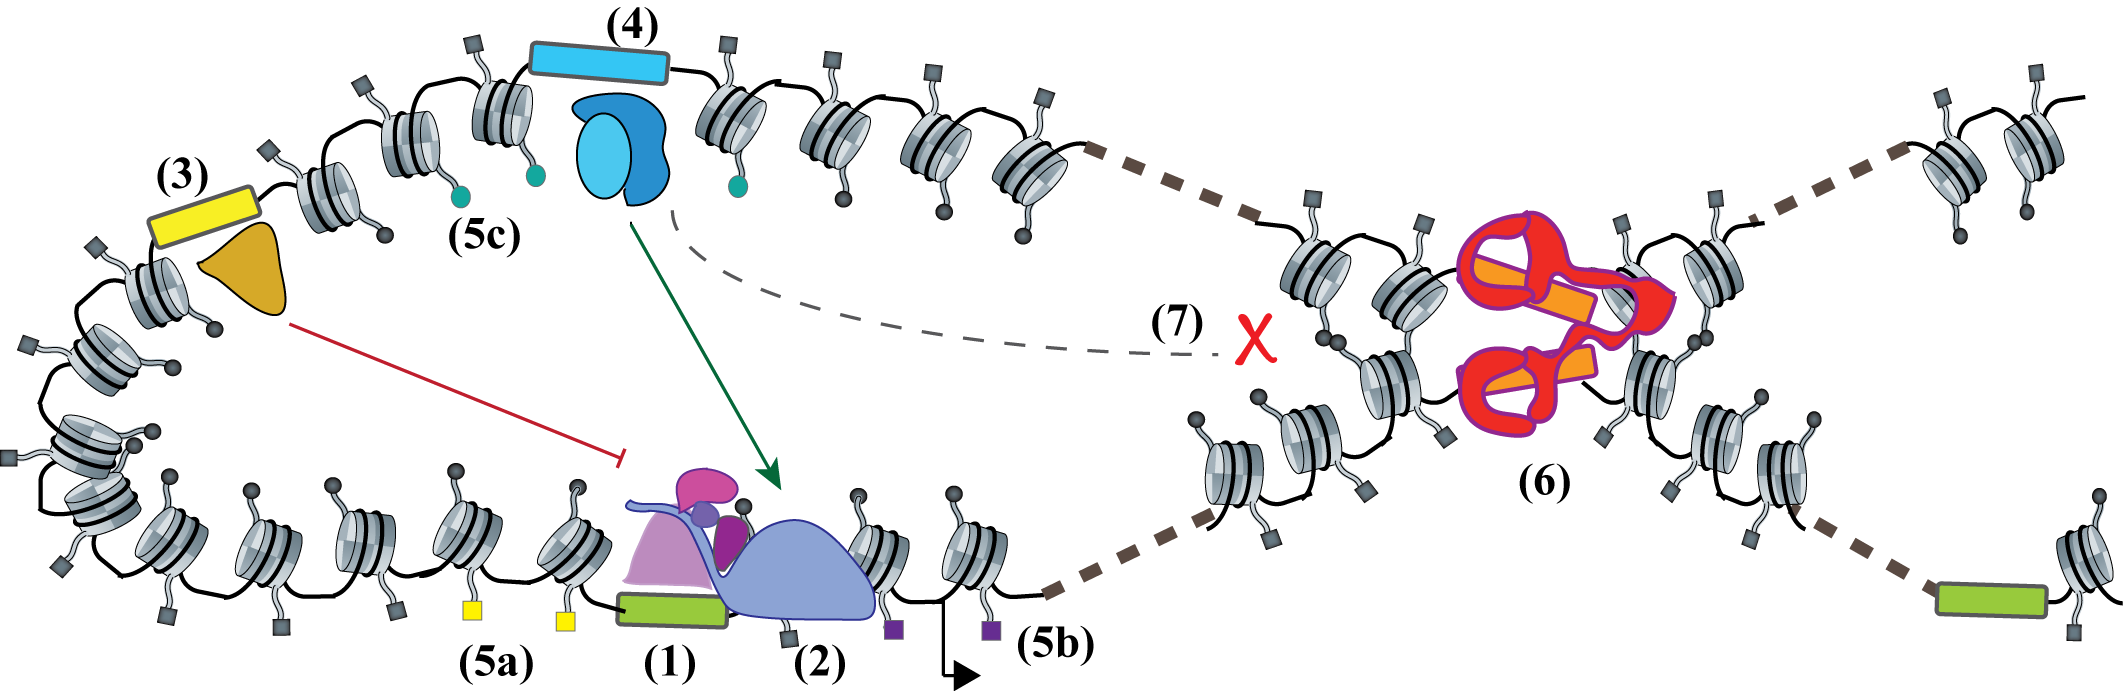
\includegraphics[width=0.8\linewidth]{figures/intro_fig1} 

}

\caption[Regulation of gene expression by various genetic and epigenetic elements]{\emph{\textbf{Regulation of gene expression by various
genetic and epigenetic elements} A promoter (1) recruits RNAP-II (2) to
perform transcription of target genes. Elements such as repressors (3)
or enhancers (4) could recruit transcription factors that either
suppress or activate gene expression. All these elements are marked by
various histone marks, such as H3K4me3 at promoters (5a) H3K36me3 at
gene bodies (5b) or H3K27ac at enhancers (5c), which facilitate gene
expression. Insulators (6) recruit proteins that facilitate DNA looping,
and block transcription factors from activating genes outside of the
established boundaries (7).}}\label{fig:unnamed-chunk-1}
\end{figure}











\subsection{Global scale : Loops, TADs, and
compartments}\label{global-scale-loops-tads-and-compartments}

Looping of DNA has been shown to be the mechanism behind long-range
enhancer-promoter interactions in the early 1990s \textsuperscript{23}.
Since then, various techniques have been developed to study long-range
interactions via chromatin looping (see section on the analyses of
chromosome conformation). Genome-wide derivation of the chromosome
conformation capture (3C) technique, called HiC \textsuperscript{24} is
currently the most popular amongst those. Early HiC studies were limited
by their resolution, and therefore discovered higher-order chromatin
structures called compartments \textsuperscript{24} and chromatin
domains, referred as \textbf{topologically associating domains (TADs)}
\textsuperscript{25}. Studies performed later revealed that chromatin is
hierarchically organized, where the domains with similar chromatin
signatures are spatially clustered. At the highest level of this
clustering, the genome can be divided into A and B
\textbf{compartments}, which separate inactive and active chromatin in
the cell \textsuperscript{24}. Compartments could further be segregated
into subcompartments that represent clustering of histone marks
\textsuperscript{26}. TADs serve as the next (lower) level of this
segregation, while enhancer-promoter loops are at the lowest level.
Functionally, TADs were shown to act as ``regulatory units'' or
``insulated neighbourhoods'', limiting enhancer-promoter interactions
and the spread of chromatin marks \textsuperscript{27}. This property of
TADs resembles those of insulators, and in fact several classically
studied insulator proteins were found to be associated with TAD
boundaries \textsuperscript{28}. Interestingly, unlike loops, which show
cell-type specific interactions \textsuperscript{29}, TADs have been
indicated to be cell-type invariant and evolutionarily conserved
\textsuperscript{25,30}.
\begin{figure}

{\centering 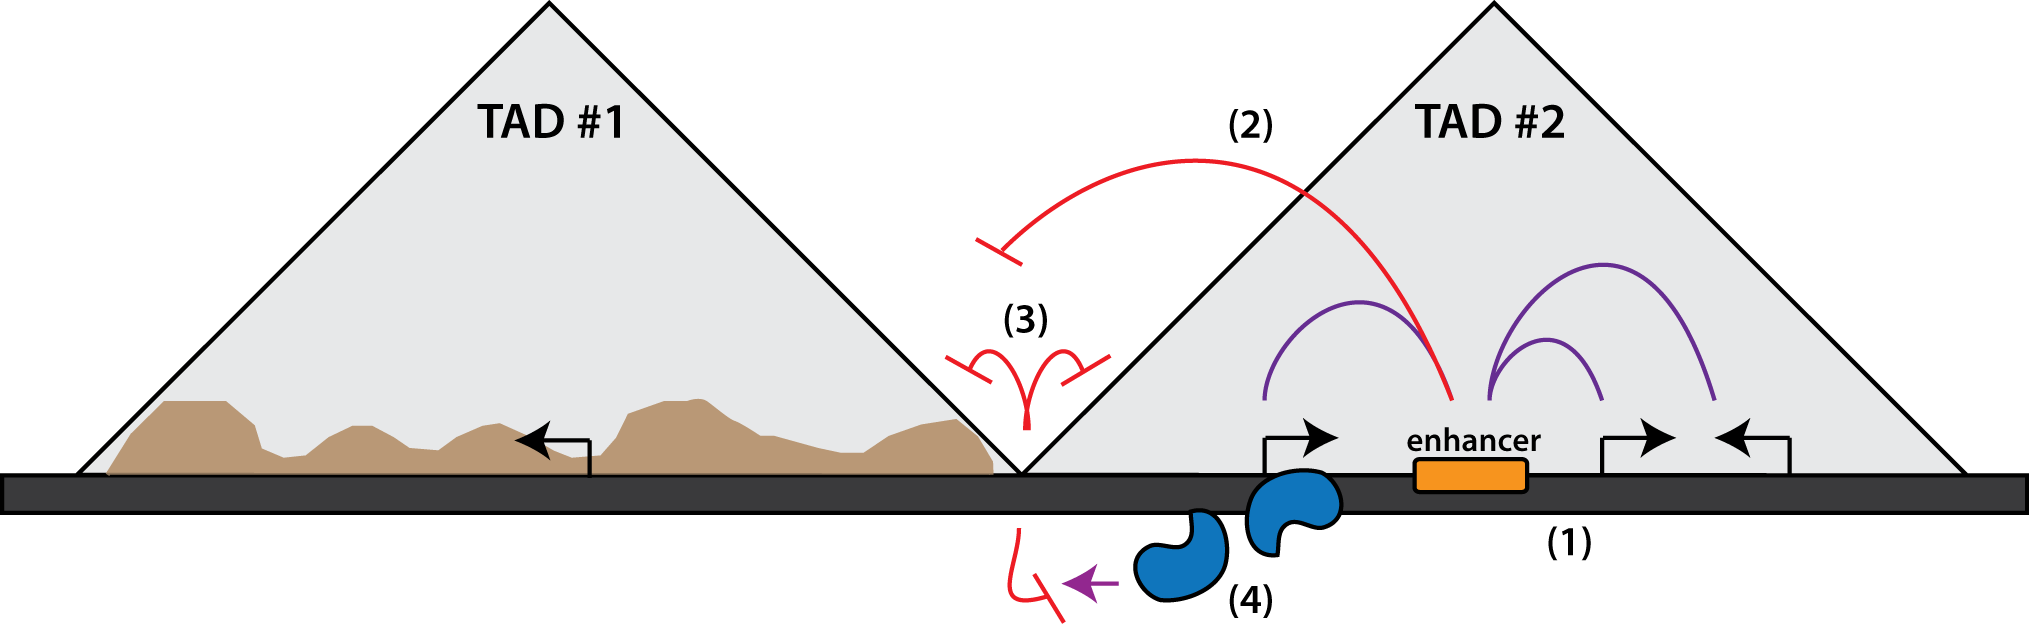
\includegraphics[width=0.8\linewidth]{figures/intro_fig2} 

}

\caption[Proposed functions of TADs in the genome]{\emph{\textbf{Proposed functions of TADs in the genome.} TADs
serve as regulatory units by providing insulated neighbourhoods for
enhancers to activate their target genes (1), blocking the enhancers
from activating the off-target genes (2), regulating the spread of
chromatin marks in cis (3) and blocking the antisense transcription from
encroaching into nearby genes (4). Figure inspired from the review by
Dixon et al. (2016) \textsuperscript{27}}}\label{fig:unnamed-chunk-2}
\end{figure}








Due to high-paced technology development, last few years have seen a
fascinating advance in our understanding of the mechanism behind loop
and TAD formation. The first study performed using in situ HiC
visualized loops as regions of enriched contacts between long distance
loci, and identified the insulator element CTCF, on loop anchors
\textsuperscript{26}. The loop anchors associated with cohesin subunits
RAD21 and SMC3, along with CTCF motifs oriented in convergent direction,
corroborating previous evidences on the role of CTCF and cohesin in
mediating DNA looping \textsuperscript{31}. Several models of loop
formation have been proposed \textsuperscript{32}. However, the
``extrusion-model'' proposing loop formation via DNA loop-extruding smc
complexes (cohesin and condensin) has received the most evidence, and
this model could also explain the 3D genome structure observed with the
HiC data \textsuperscript{33--35}. Also, the \emph{in-silico} models
produced by the Mirny lab have proposed loop extrusion as a common
mechanism behind formation of loops, TADs and chromosomal compartments
\textsuperscript{36--38}. Despite all the \emph{in-silico} evidence, the
\emph{in-vivo} evidence linking extrusion to loop formation was lacking,
until the studies perturbing loop-associated factors emerged. A
depletion of CTCF eliminated CTCF associated loops in the genome
\textsuperscript{39}, while the depletion of cohesin eliminated all loop
domains \textsuperscript{40}. A CRISPR mediated knockout (KO) of the
cohesin release factor WAPL showed that the duration of association of
cohesin complex (SCC2/SCC4) determines the length of loops
\textsuperscript{41}. These studies reinforced a common mechanism behind
loop and TAD formation. However, surprisingly, they also showed that
compartments as well as histone marks remain unaffected upon loop
depletion, suggesting an independent mechanism behind the segregation of
compartments. Another interesting point about studies linking cohesin
and loop extrusion is that they don't explain how cohesion physically
extrudes chromatin, since no \emph{in-vivo} extrusion activity of
cohesin complex has been visualized \textsuperscript{42}. Another smc
associated protein, condensin, however, has been shown to have the motor
activity \textsuperscript{43} and recently, its \emph{in-vivo} loop
extrusion activity has also been visualized \textsuperscript{44}.

Single molecule imaging suggests that although cohesin can undergo rapid
diffusion along DNA, its mobility is highly restricted by nucleosomes,
and the DNA motor proteins can readily push cohesin along DNA
\textsuperscript{45}. On the same line, transcription has been proposed
as a mechanism behind cohesin mediated loop extrusion
\textsuperscript{42}. HiC studies showed that housekeeping genes are
enriched at TAD boundaries \textsuperscript{25,46} providing further
evidence linking transcription and TADs. A study last year showed that
TADs could emerge in absence of transcription in flies, challenging the
speculation of a causal link between transcription and TAD formation
\textsuperscript{47}, however another recent study showed that
transcription could affect 3D genome structure by displacing cohesin
from CTCF sites \textsuperscript{48}. Therefore, more research to
investigate the association between transcription and 3D genome would be
required.

\subsection{Mammalian X-inactivation : an interplay between multiple
levels of epigenetic
regulation}\label{mammalian-x-inactivation-an-interplay-between-multiple-levels-of-epigenetic-regulation}

The process of mammalian X-chromosome inactivation (XCI) serves as an
excellent example of how multiple levels of epigenetic regulations act
in synchrony and influence each other. Mammals (as well as
\emph{Drosophila}) have XX-XY form of sex determination, leading to an
imbalance of X-chromosome gene dosage between sexes. This imbalance is
corrected by an epigenetic phenomenon (dosage compensation) where one of
the female X-chromosomes is randomly inactivated during differentiation
\textsuperscript{49}. In mouse, XCI happens in two waves, an imprinted
paternal XCI is established at 4-8 cell stage, and the paternal X
remains inactive in trophectoderm but is reactivated in the inner cell
mass of the blastocyst (ICM) \textsuperscript{50}. This is followed by
the random XCI, which coincides with the downregulation of pluripotency
factors such as Nanog, Oct4/Pou5f1 and Sox2 \textsuperscript{51}. The
embryonic stem cells (ESCs) derived from the ICM, serve as a good model
to study XCI, since XCI can be achieved simply by inducing ESC
differentiation \textsuperscript{52}.

The X-inactivation center (Xic) is a locus on X-chromosome which is
required to trigger XCI \textsuperscript{53}. Xic contains the
non-coding RNA Xist, which coats the inactivating X-chromosome during
XCI. Xist is negatively regulated by its antisense RNA Tsix, and
positively regulated through a ubiquitin ligase Rnf12, in a
dosage-sensitive manner \textsuperscript{54}, both of which are
controlled by the pluripotency factors \textsuperscript{55,56}. On Xic,
multiple putative regulators of Xist, such as Rnf12, Jpx, Ftx and Xpr
have been shown to be important for specific targeting of X-chromosome
for the inactivation process (referred as ``sensing'')
\textsuperscript{57}. The mechanism behind selection of one of the two
X-chromosomes for inactivation (referred as ``choice'') remains elusive,
although in mouse, Tsix has been suggested to be important for the
process. A potential mechanism of action of Tsix could be that transient
pairing of X-chromosome during ESC differentiation \textsuperscript{58}
somehow leads to an asymmetry in Tsix expression, followed by
recruitment of repressive chromatin marks \textsuperscript{59}, which in
turn leads to the asymmetry in Xist expression.

During XCI, the Xist RNA coats the X-chromosome, which results in
depletion of RNAP-II and the activating histone marks, such as H4
acetylation \textsuperscript{60}. The Xist coated chromatin then gets
enriched in repressive chromatin marks such as H2AK119ub, H3K9me and
H3K27me3 \textsuperscript{61,62}. It's been proposed that Xist silencing
followed by H2AK119ub could in turn recruit PRC1, which could indirectly
recruit PRC2 through Jarid2, bringing in H3K27me3 \textsuperscript{63}.
This rapid change of chromatin state is accompanied by a change in 3D
conformation. The X-linked genes initially reside in nuclear periphery,
outside the repressive nuclear compartment, and get recruited into it
during inactivation \textsuperscript{64}. Ultimately, the inactive-X is
condensed to a heterochromatic form, known as the barr body
\textsuperscript{65}. The mechanism of Xist spreading has been
investigated using RNA immunoprecipitation (RAP and CHART-seq)
techniques, which suggested that Xist could exploit the chromosome
conformation to spread to regions in spatial vicinity
\textsuperscript{66,67}. It's due to this intricate interplay of
chromatin, non-coding RNA and chromosome conformation that recent
studies studying XCI have turned to multi-assay epigenomic techniques
\textsuperscript{68,69}. It's evident that similar integrative studies
would be required in future to study XCI and other such multi-step
phenomena.

\section{Regulation of transcription by the MSL
complex}\label{regulation-of-transcription-by-the-msl-complex}

\subsection{Dosage compensation in flies via the MSL
complex}\label{dosage-compensation-in-flies-via-the-msl-complex}

In \emph{Drosophila}, dosage compensation is achieved by the
upregulation of the single X-chromosome in males \textsuperscript{70}.
Males absent on first (MOF), an enzyme that specifically deposits
acetylation marks on Histone H4 Lysine 16 (H4K16ac) is required for the
process \textsuperscript{71}. MOF associates with the male-specific
lethal (MSL) complex, containing proteins MSL1, MSL2, MSL3, MLE
(maleless) RNA helicase, and non-coding RNAs roX1 and roX2. roX1 and
roX2 are lncRNAs containing stem-loop structures which are expressed
from the X-chromosome and seem to play a redundant role in dosage
compensation \textsuperscript{72}. The E3 ubiquitin ligase MSL2 is only
expressed in males and, in association with roX RNAs, provides
specificity of the complex towards X-chromosome \textsuperscript{73,74}.
Binding specificity to certain DNA motifs by the MSL2 CXC domain has
been shown to bring X-specificity \textsuperscript{75}. MSL1 serves as a
scaffold for binding to other proteins in the complex, and plays an
essential role in the assembly of the complex via its homodimerization
and DNA binding property \textsuperscript{76}. MSL3 enhances the
acetylation activity of MOF \textsuperscript{77} and contains a
chromodomain which facilitates the spread of the complex towards gene
ends \textsuperscript{78}. Finally, the MLE helicase stabilizes the roX
RNAs and is important for its incorporation into the complex
\textsuperscript{79}.

Studies have shown that following this multi-step assembly process, the
complex is first recruited to certain specific loci on the X-chromosome,
referred to as high-affinity sites (HAS), followed by further spreading
to nearby loci \textsuperscript{80}. Sites of roX RNA expression serve
as strong high-affinity sites. Further, the complex decorates the
X-chromosome and deposits H4K16ac on promoters, gene bodies, as well as
intergenic regions. The increase in H4K16ac has been shown to enhance
transcription \textsuperscript{81}. Multiple studies have investigated
the precise mechanism of this transcriptional enhancement using
genome-wide techniques such as ChIP-seq \textsuperscript{82}, GRO-seq
\textsuperscript{83} and nascent RNA-seq \textsuperscript{84}. These
evidences point out that transcriptional upregulation is a joint result
of increased RNAP-II recruitment as well as processivity.

\clearpage
\begin{figure}

{\centering 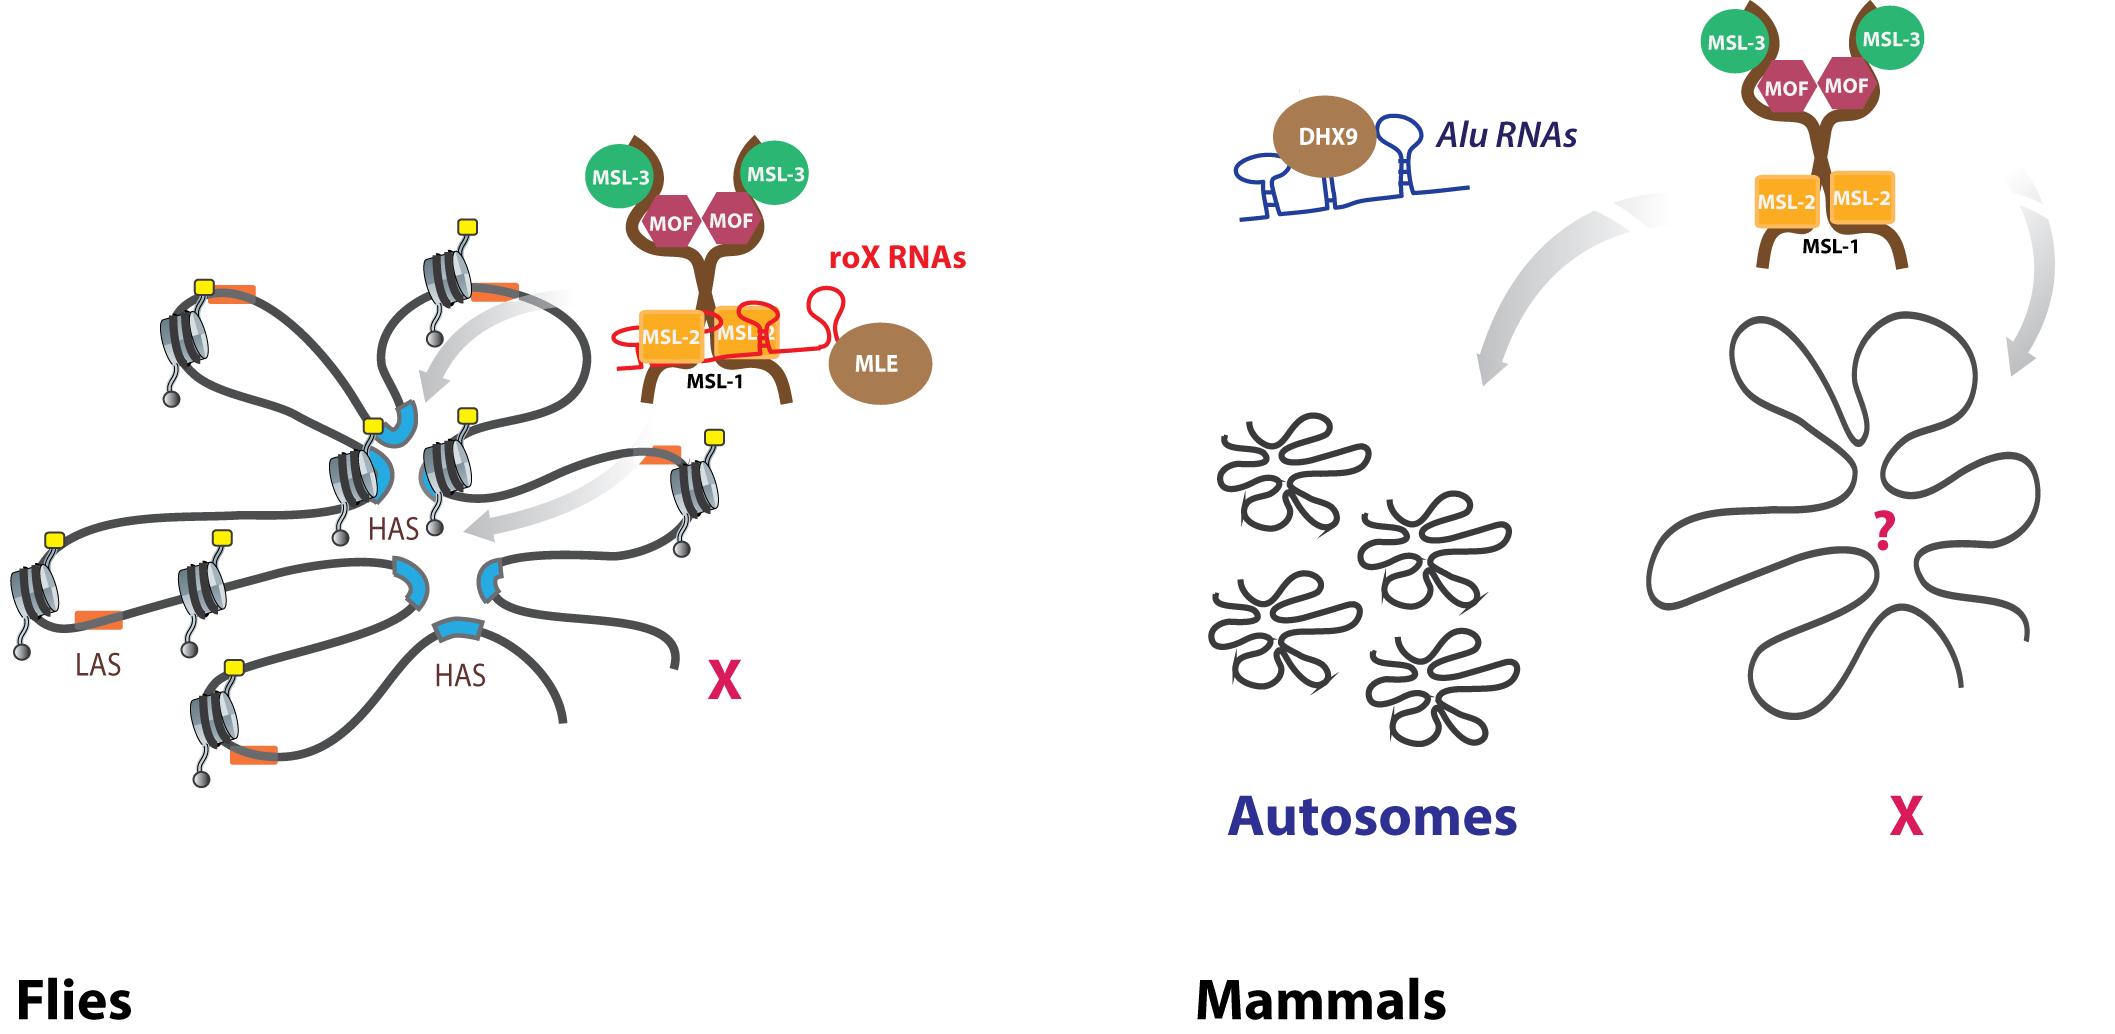
\includegraphics[width=0.9\linewidth]{figures/intro_fig3} 

}

\caption[Functions of the MSL complex in flies and mammals]{\emph{\textbf{Functions of the MSL complex in flies and
mammals.} In \textbf{flies}, the MSL complex assembles in presence of
the roX RNAs, whose secondary structures are recognized and resolved by
the maleless helicase (MLE), the complex then targets the high-affinity
sites (HAS, blue) containing roX. The HAS cluster in 3D space, allowing
efficient targeting by MSLs. The complex then spreads to low affinity
sites (LAS, orange), depositing H4K16ac marks (yellow) on the X. In
\textbf{mammals}, roX RNA is absent and the complex is believed to
assemble in absence of any RNAs, and targets both, X and autosomal
sites. Specificity towards the X-chromosome, as well as the role of
chromosome conformation is unknown so far. MLE homolog DHX9 associates
with a separate class of RNAs and performs independent functions
(presented in results). Figure inspired from \textsuperscript{88}}.}\label{fig:unnamed-chunk-3}
\end{figure}














There are interesting parallels between \emph{Drosophila} and mammalian
dosage compensation systems. Both systems rely on an lncRNA expressed
from the X-chromosome, which seem to be important for the recognition of
the chromosome (\textbf{sensing}), and both of them rely on a global
deposition of histone marks which associates with suppression or
hyperactivation of genes. In \emph{Drosophila} however, the problem of
\textbf{choice} seems to be simplified, since the compensation occurs on
the single male X-chromosome and the male-specific expression of MSL2
assures the sex-specificity. Nevertheless, this similarity suggests that
questions in one species could be tackled by learning from another. For
example, in parallel with the role of chromosome conformation in guiding
the spread of Xist RNA, research performed in our lab and by others have
shown that the spreading of the MSL complex on the X-chromosome is
guided by the 3D spatial proximity of HAS \textsuperscript{85,86}. These
observations also lead to further interesting questions. For example,
studies have shown that despite a global inactivation of the
X-chromosome, about 15\% of genes in humans and a 3\% in mice, escape
inactivation (referred to as escapees) \textsuperscript{87}. Escapee
biology has been heavily studied in mammals, however studies to
investigate whether different genes might also respond differently to
dosage compensation has been lacking in flies.

\subsection{Functions of MOF and MSL complex in
mammals}\label{functions-of-mof-and-msl-complex-in-mammals}

Proteins of the MSL complex are conserved from flies to humans, and
evidence suggests that MOF is responsible for the majority of H4K16ac
\textsuperscript{89}. Human homologs of MSL1, MSL2, MSL3 and MOF have
been co-purified, suggesting that the bulk of the MSL complex stays
together. It's compelling to speculate that role of MSL complex along
with the role of H4K16ac might have diverged, considering that mammalian
dosage compensation works via a different mechanism, and no ortholog of
roX RNAs have been discovered on the X-chromosome so far
\textsuperscript{90}. However, there is evidence that the active
X-chromosome in mammals might also be upregulated
\textsuperscript{91,92}, and a recent study has supported the role of
MOF mediated H4K16ac in enhancing transcription on a subset of X-linked
genes \textsuperscript{93}. Apart from its association with dosage
compensation, MOF mediated H4K16ac has also been implicated in
embryogenesis and oncogenesis \textsuperscript{90,94}. However, it
should be noted that MOF is also associated with another complex, called
the non-specific lethal (NSL) complex, which is conserved from flies to
humans, and is involved in depositing H4K16ac on housekeeping and
constitutively expressed genes \textsuperscript{95}. Therefore, some
functional outcomes of H4K16ac could relate to the MOF-MSL complex,
while others to the MOF-NSL complex \textsuperscript{96,97}.

In flies, the MOF-NSL complex is shown to be responsible for the bulk of
H4K16ac on the gene promoters, while the MSL complex deposits the mark
on gene bodies of the X-chromosome. A recent study from our lab showed
that in mammals, however, MSL and NSL proteins colocalize on promoters
of target genes on both X and autosomes \textsuperscript{96}. The study
also showed that the MSL mediated H4K16ac contributes to the regulation
of Tsix expression and the depletion of MSLs in ESCs leads to chaotic
XCI during their differentiation. However, the lack of specificity
towards the X-chromosome and co-localization with NSL proteins at the
promoters raise further questions about the specific genome-wide role of
the MSL complex, as well as its role on the mammalian X-chromosome.

Apart from the MSL complex, the human ortholog of MLE helicase, DHX9, is
also conserved in mammals, and has been shown to unwind both DNA and
double-stranded RNA \textsuperscript{98--100}. However, in absence of
its association with the MSL complex, the function of its RNA helicase
activity in mammals had not been studied in detail. A study presented in
this thesis investigates the RNA binding partners of DHX9 in mouse and
humans, and proposes a novel evolved function of DHX9 in suppression of
undesired expression of RNAs \textsuperscript{101}.

\section{High-throughput techniques to study transcriptional
regulation}\label{high-throughput-techniques-to-study-transcriptional-regulation}

Due to consistently reducing costs of sequencing, increase in our
ability to multiplex many samples, and sequence genetic material from as
low as a single cell, a large number of biologists now rely on
genome-wide assays for their research. Researchers have quickly realized
that the ability to store, process, analyze, interpret and visualize
this data would become a major challenge for biology
\textsuperscript{102}. Below I will focus on recent developments in
techniques employed for the study of DNA-protein interactions,
chromosome conformation and transcription.

\subsection{ChIP-seq : current standards and
challenges}\label{chip-seq-current-standards-and-challenges}

Chromatin Immunoprecipitation followed by sequencing (ChIP-seq) is a
broadly used method to detect genome-wide protein-DNA interactions in
cells \textsuperscript{103}. ChIP-seq allows us to probe genome-wide
binding sites for TFs, or study the distribution of histone marks. It
has led to numerous discoveries and has been used by large consortia
such as ENCODE, to map cell-type specific regulatory elements such as
enhancers in the human genome \textsuperscript{17}. A ChIP-seq
experiment involves DNA-protein cross-linking (using UV or
formaldehyde), chromatin fragmentation (using sonication or enzymes),
purification of DNA-protein crosslinks with or without antibody (called
``ChIP'' and ``input'' DNA), and high-throughput sequencing of
associated DNA. Since the technique involves cross-linking, shearing,
and affinity based pull-down, the data obtained from the protocol is
directly affected by three major factors : 1) \textbf{cross-linking
efficiency} of proteins might be influenced by their nature of DNA
binding (direct vs indirect, transient vs stable) 2) \textbf{stability}
of the protein epitope under shearing and washing conditions would
affect enrichment and 3) \textbf{antibody cross-reactivity} could result
in detection of non-specific interactions \textsuperscript{104,105}.
Variations of ChIP-seq protocols as have been developed to tackle these
biases, such as MNase-ChIP \textsuperscript{106}, to account for
shearing and stability bias, and DamID-seq \textsuperscript{107} to
account for antibody bias. Further, variants such as iChIP
\textsuperscript{108}, Mint-ChIP \textsuperscript{109} and RELACS
\textsuperscript{110} aim to increase the multiplexing ability and allow
reducing the number of cells. Such methods might receive more popularity
in the future.

The analysis of ChIP-seq data involves mapping of sequenced DNA to a
reference genome, and detection of regions enriched in ChIP DNA (called
``Peaks'') using input DNA as a negative control. Peaks represent the
``detected'' binding sites of the TF or histone mark of interest. These
peaks are then used to find DNA binding motifs for the TFs, detect
target genes, and integrate these results with other assays (such as
RNA-seq) to understand gene regulation \textsuperscript{111}. Apart from
the sources of bias described above, the sequencing depth or genomic
nucleotide content (GC bias) could lead to sample-specific bias in
ChIP-seq, and various ``normalization'' methods have been developed to
account for such biases \textsuperscript{112--115}. Our group previously
developed ``deepTools'' \textsuperscript{116}, a set of tools that allow
users to identify biases and perform such normalizations, and visualize
the downstream results in a user-friendly manner. However, due to
improvements in experimental and analysis methods, new challenges have
emerged as previous issues have been resolved. Specifically, increase in
multiplexing ability has simplified performing routine large-scale
experiments \textsuperscript{110}, and the demand for user-friendly
tools for differential ChIP-seq analysis between conditions
\textsuperscript{117}, quantitative normalization using external
controls \textsuperscript{118,119}, and large-scale processing and
integration of datasets has been increasing. The development of tools
that allow multi-sample comparison and integration of quality control
and analysis would be widely appreciated. This was the motivation behind
our recent update of deepTools \textsuperscript{120}.

\subsection{Analyses of chromosome
conformation}\label{analyses-of-chromosome-conformation}

Past 10 years have seen lots of development in genome-wide techniques to
capture physical interactions between chromatin loci inside the cell.
The first popular measure to detect chromatin interactions between loci
was called \textbf{3C} (chromosome conformation capture). 3C involved
cross-linking the chromatin such that the regions in spatial proximity
inside the nucleus get linked to each other, followed by the digestion
of chromatin using restriction enzymes (REs) and the ligation of
close-by DNA fragments. These ligated fragments could then be amplified
using qPCR primers specific to the region of interest, to measure
interaction frequency \textsuperscript{121}. 3C was extended to 4C,
where all regions interacting with a locus of interest (referred to as
``bait'') could be detected by inverse PCR using outward facing primers
on the 3C-ligated product, followed by hybridization to a microarray
chip to detect interactions \textsuperscript{122}. The 5C technique
introduced later used highly multiplexed ligation-mediated amplification
(LMA) to first ``copy'' and then amplify parts of the 3C library
followed by detection via microarrays or sequencing
\textsuperscript{123}. Finally the genome-wide version of 3C, called
HiC, involved biotin-based pull down of 3C fragments, followed by
library preparation and paired-end sequencing of the enriched fragments
\textsuperscript{24}. An improved version of HiC protocol performs
restriction digestion and ligation of 3C fragments inside intact nuclei,
avoiding non-specific interactions. This technique, referred as in situ
HiC \textsuperscript{26} is currently the most popular method for
genome-wide detection of chromatin contacts.

All the 3C-based methods however, suffer from two issues : 1) The
cross-linking of chromatin makes the technique less quantitative and
proximity ligation introduces additional biases; 2) These methods only
allow detection of pair-wise contacts between two genomic bins. Due to
its limitations and biases, together with the observed discrepancy
between 3C and microscopy-based visualization of interactions, the
interpretation of 3C-based proximity as real molecular proximity has
been questioned \textsuperscript{124--126}. Recent innovations in
chromosome conformation techniques, such as GAM \textsuperscript{127},
SPRITE \textsuperscript{128} and damC \textsuperscript{129} have tried
to overcome these limitations. SPRITE is particularly interesting since
it detects multi-loci chromatin interactions via a relatively simple
split-pool barcode tagging of the cross-linked chromatin fragments, and
can also detect DNA-RNA interactions \textsuperscript{128}. It's not
unlikely that one of these new innovations might replace in situ HiC as
the primary method for the analysis of 3D genome.

HiC libraries are sequenced as paired-end, where ideally, one read in a
pair comes from one of the interacting loci in the genome while the
second read comes from another \textsuperscript{24}. However, due to the
issues with ligation efficiency, biotinylation and IP of the interacting
pairs, many ``invalid'' HiC pairs also get sequenced. Analysis of HiC
data begins with separate \textbf{mapping} of the two reads in a pair,
followed by pairing and \textbf{filtering} of reads. To consider a pair
``valid'', two reads should come from different fragments which were
ligated during the protocol, and therefore should have a restriction
site in between them. After filtering of valid pairs, the genome is
divided into bins, and the number of paired-end contacts between all
bins are calculated to create a \textbf{HiC matrix}.

Initial HiC protocols used whole cell lysis along with REs such as
\textbf{Hind-III}, with low cutting frequency, leading to low-resolution
HiC matrices. In contrast, the use of REs with high cutting frequencies
such as \textbf{Dpn-II} (4-cutters) combined with other improvements,
the recent in situ HiC protocols has allowed us to create higher
resolution matrices. In either case, the highest resolution matrices
could be obtained by using restriction enzyme cut-sites as ``bins'' in
the genome \textsuperscript{85,130}.

Several known and unknown factors in the HiC protocol could affect
interpretation of the observed data. Normalization methods have been
developed to explicitly account for some biases, such as the effective
length bias (due to the size of the restriction fragment), GC content
bias, and the mappability bias \textsuperscript{131,132}. However since
not all source of biases are known in the experiments, the matrix
balancing methods, which try to account for both known and unknown
biases, have been most popular \textsuperscript{133}. Matrix balancing
methods, such as ICE (Iterative Correction and Eigenvector
decomposition) \textsuperscript{134}, and Knight and Ruiz method
\textsuperscript{26,135}, assume uniform visibility of all genomic loci
and therefore ensure equal sum of row and column values. Both methods
have been shown to be useful in the analysis of HiC data.

HiC interaction matrices reveal that loci which are closer on the linear
genome also tend to interact more frequently. In normal interphase
cells, a distance dependent decay of interactions is observed, which
follows a power law. This interaction is disrupted in mitotic
chromosomes, which represent a reduction of short-range and an increase
in long-range interactions \textsuperscript{136}. It also served as a
quality control signal for the comparison of normal samples. However,
the interaction frequency could also get exaggerated due to nonspecific
proximity ligation effects, and therefore for some analysis, such as
detection of chromosomal compartments, a correction of proximity
ligation effect is needed in addition to ICE correction.
\begin{figure}

{\centering 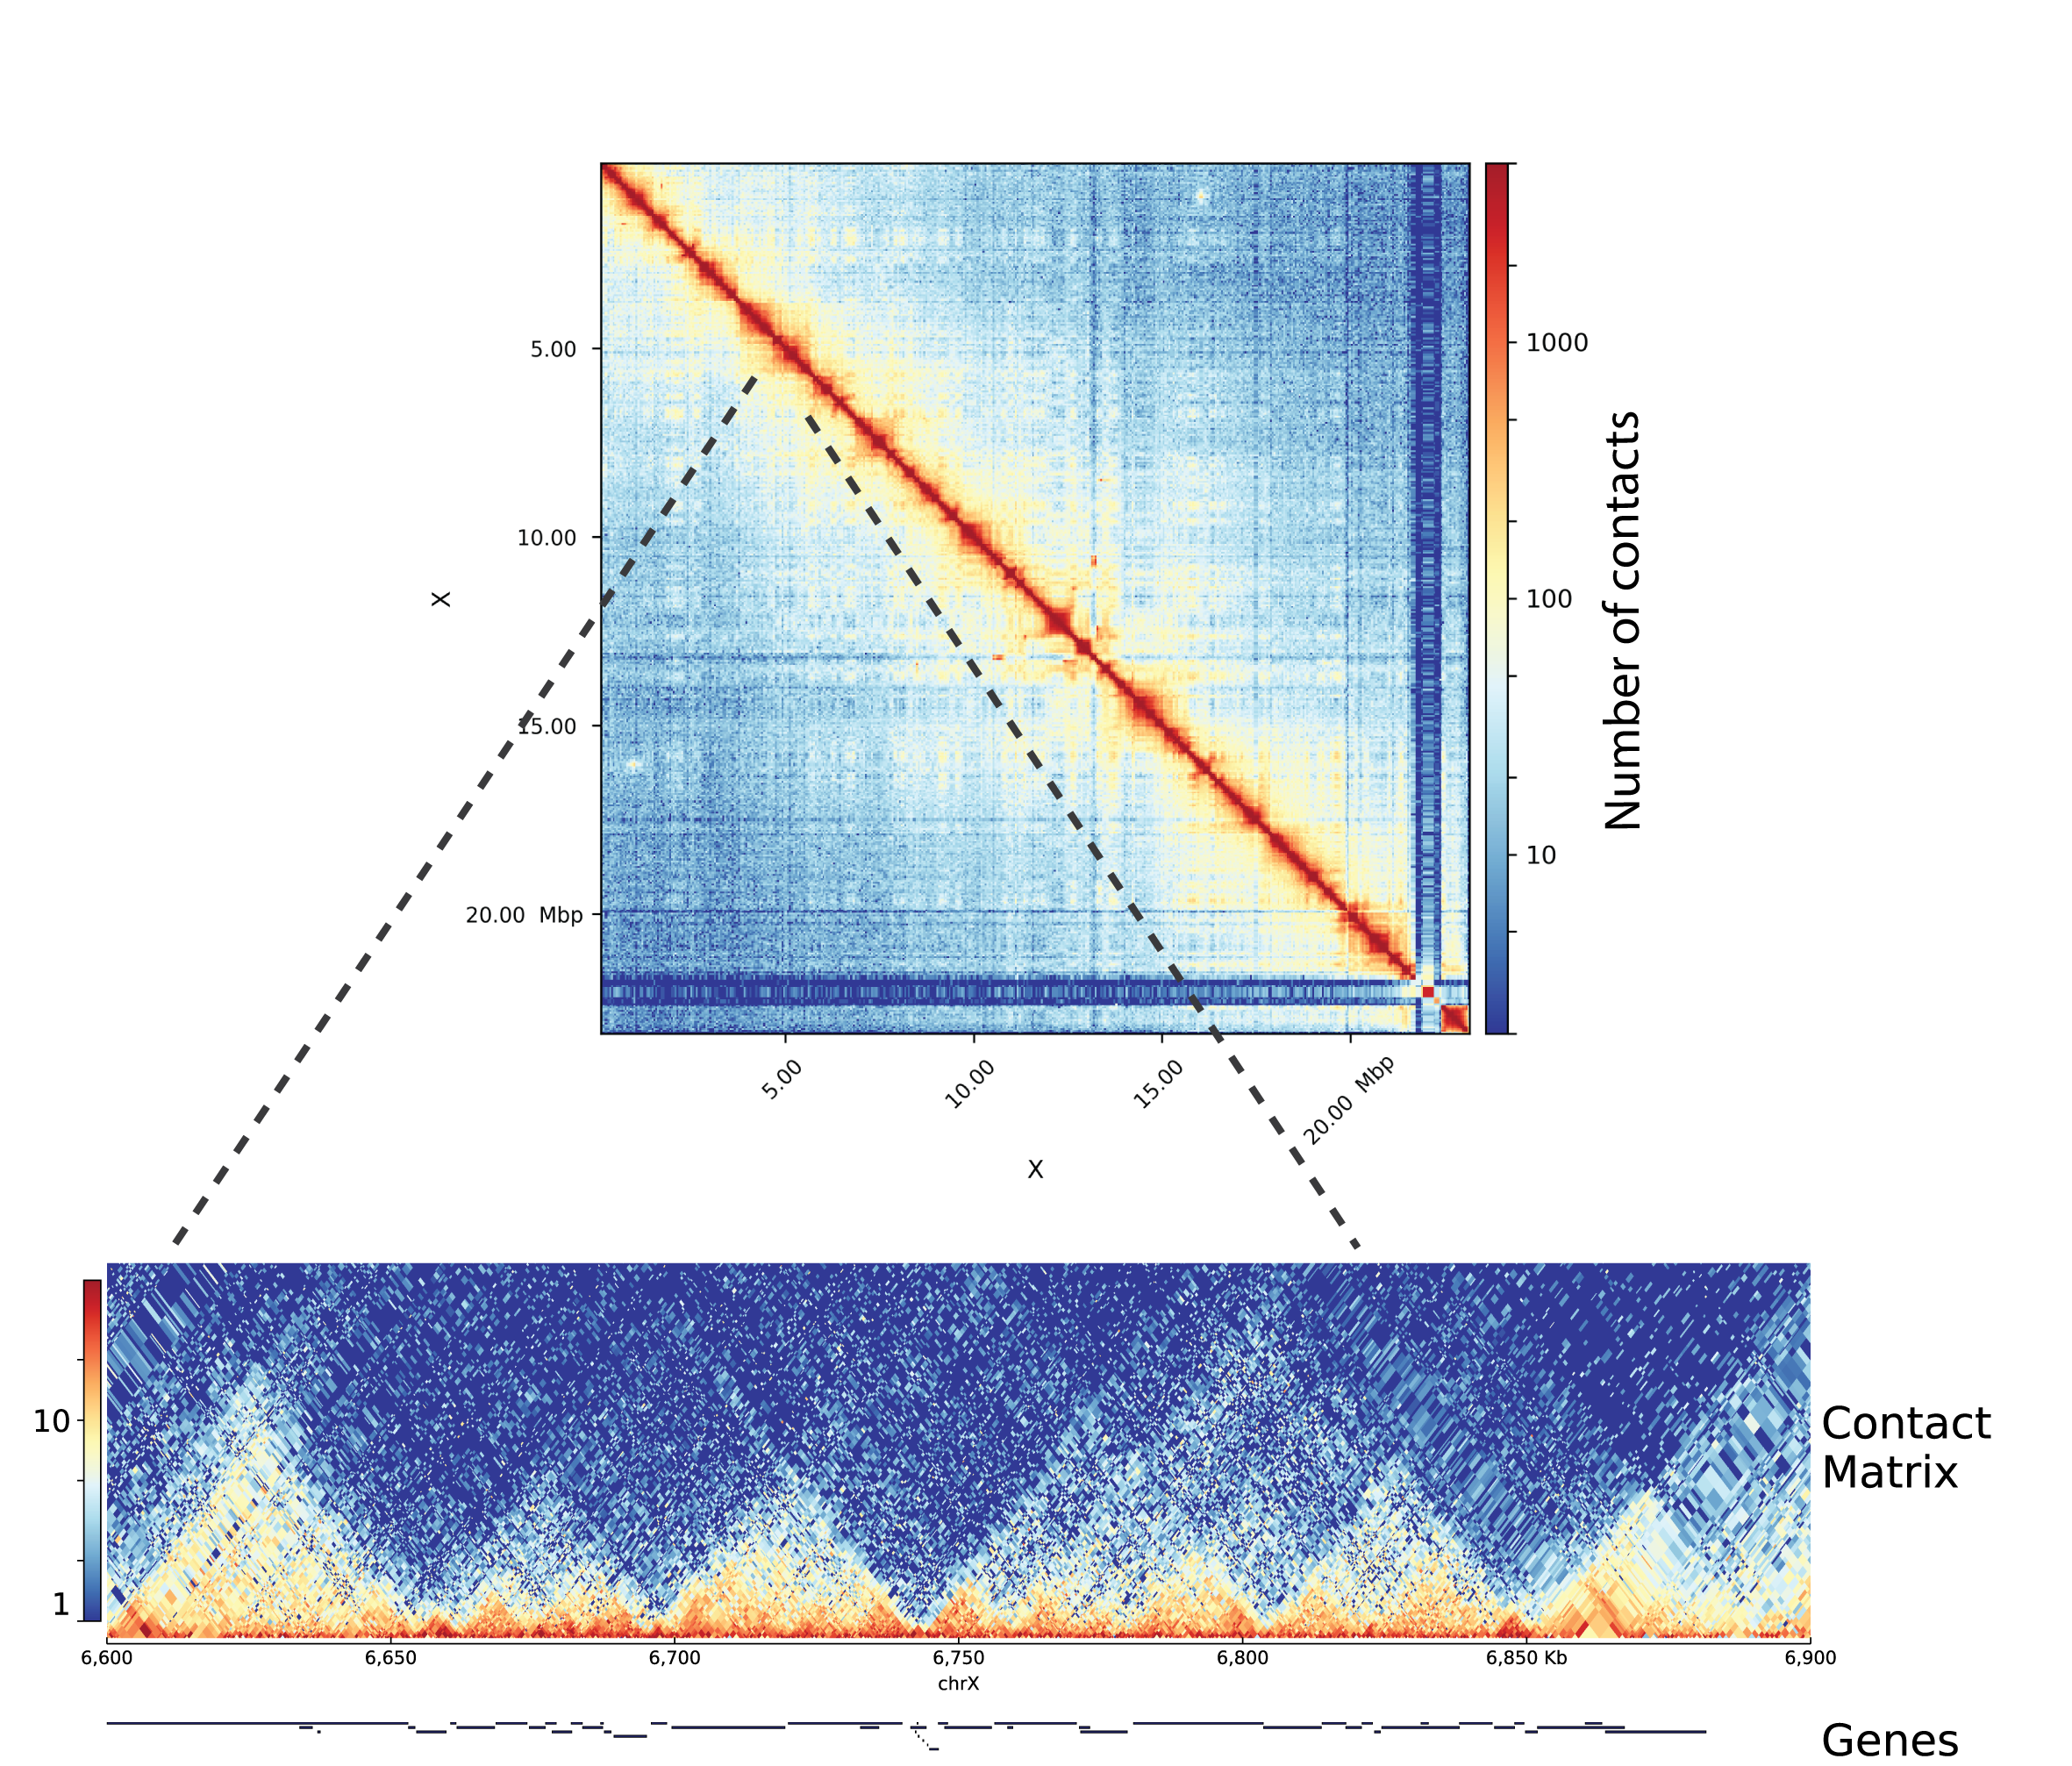
\includegraphics[width=0.8\linewidth]{figures/intro_fig4} 

}

\caption[Visualization of a normalized HiC contact matrix]{\emph{\textbf{Visualization of a normalized HiC contact
matrix.} The HiC matrix \textbf{(top)} represents all-to-all contacts
between bins in the genome, and is therefore symmetric. After cutting
the matrix from the diagonal and rotating it \textbf{(bottom)}, domains
(TADs) in shape of triangles become visible.}}\label{fig:unnamed-chunk-4}
\end{figure}






Normalized HiC matrices could be used for detection of TADs, loops,
compartments, modeling of 3D genome and visualization of genomic
interactions. Numerous software solutions have been developed over the
last few years for the processing and analysis of HiC data that allow
these applications (Appendix B2, Table-2). Detection of loops and
compartments have been formalized better than TADs due to their distinct
properties. The original method for detection of chromosomal
compartments \textsuperscript{24} assumes that regions with shared
neighbourhood have correlated interaction profiles. It therefore
transforms the HiC matrix into a correlation matrix, followed by
partitioning of chromosomes into regions of correlated interactions
using principal component analysis (PCA). This method has now been
implemented in multiple tools (Appendix B2, Table-2). The method used
for genome-wide detection of loops utilizes high-resolution in situ HiC
data and searches for clusters of matrix entries with enriched
interactions relative to a local background. This method, referred to as
HiCCUPs \textsuperscript{26}, has been implemented in the Juicer
pipeline \textsuperscript{137}.

Methods for detection of TADs have been evolving fast over the last few
years. The first group describing TADs \textsuperscript{25}, observed
that within a TAD the bins closer to the boundary have a high
interaction bias towards bins in the middle. They developed a metric
that quantified the contacts of a bin with a larger region upstream (A)
and downstream (B) of that bin and compared it to the contact
probability expected under a null distribution of \emph{(A+B)/2}. This
\emph{directionality index} (DI) was used as an observation to infer the
true directionality bias via a hidden markov model (HMM), which
predicted the TADs. Later, methods based on maximum likelihood
segmentation \textsuperscript{138}, breakpoint detection
\textsuperscript{139}, and hierarchical clustering \textsuperscript{140}
were developed. In principle, all these methods formalize the
observation that TADs are visualized as domains of enriched contacts
relative to their neighbourhood on a HiC matrix, and try to produce the
most similar set of predictions corresponding to this visual
observation. Multiple studies showed that genome organization is
hierarchical, and TADs have been speculated to be the level of this
hierarchy which are not structurally, but rather functionally privileged
\textsuperscript{140,141} . Therefore ideal methodology for TAD
detection has still not been settled, and the benchmarking of TAD
calling methods rely on visual identification of true positives
\textsuperscript{142}.

\subsection{Transcript profiling methods and
analyses}\label{transcript-profiling-methods-and-analyses}

Transcriptomics (study of all transcripts in the cell), has been one of
the most popular fields where NGS is being applied. The most widely used
bulk RNA-seq methods (studying a population of cells) are poly-A or
ribo-depleted RNA-seq. In \textbf{poly-A} RNA-seq, oligos are used to
enrich for mRNA (containing poly-A tails) while in
\textbf{ribo-depleted} RNA-seq, all RNAs (except ribosomal RNA) are
sequenced \textsuperscript{143}. Ribo-depleted RNA-seq allows for
analysis of poly-A along with non poly-A RNA, such as unprocessed
transcripts and RNAP-III transcribed RNAs. However, detection of all
kinds of RNA requires a high depth of sequencing, the capacity of
sequencing library to capture transcripts of various lengths, and enough
input material from the cells to avoid RNA composition effect (masking
of lowly expressed transcripts by the abundant RNA). Methods have been
developed to enrich for specific RNA species in the cell, such as small
(\textless{}50 nt) RNAs \textsuperscript{144}, transiently transcribed
RNAs \textsuperscript{145} , and circular RNAs \textsuperscript{146}.

The analysis of RNA-seq data \textsuperscript{147} includes
\textbf{trimming} adaptors and low quality bases from single or
paired-end reads, followed by \textbf{mapping} of the reads to a
reference genome. Genomic mapping of RNA-seq requires splice-aware
alignments (allowing for splitting of reads mapping to splice junctions,
in order to map across introns). In order to obtain the estimate of
transcript numbers in the cells, counting and \textbf{summarizing} of
reads is performed afterwards, using gene annotations as reference.
Usually, RNA-seq is performed on multiple biological \textbf{replicates}
of two or more groups (control vs knockdown, tissue 1 vs tissue 2 etc.),
in order to find genes or transcripts that vary significantly between
the groups (called \textbf{differential expression} analysis).
Differentially expressed genes are used to look for functional
enrichments of gene categories using methods like Gene Ontology (GO)
analysis \textsuperscript{148}. Gene level differential expression
analysis has been standardised in the field, while methods for
quantification and differential expression of transcript isoforms are
still under active research \textsuperscript{149}. A special case of
differential expression is where a large number of transcripts are
affected, such as knockdown of TFs regulating housekeeping genes, or
genome-wide transcriptional activation/repression \textsuperscript{150}.
These cases require normalization using external, non-changing controls
referred to as \textbf{spike-ins} \textsuperscript{151}. For special
applications of RNA-seq such as detection of \textbf{circular RNAs}, the
mapping and summarization of reads requires an entirely different
strategy, and various tools have been developed to facilitate this
\textsuperscript{152}. Another special application of RNAseq is for the
identification of \textbf{RNA editing} \textsuperscript{153}, which
require stringent mapping and variant detection followed by multiple
rounds of filtering. Due to evolving standards, these applications still
rely on custom analysis.

Although RNA-seq has helped with genome-wide annotation of transcripts
in the genome, it requires fragmentation of RNA, making it difficult to
accurately detect transcription start sites (TSSs) and perform promoter
profiling. Techniques for promoter profiling, such as Cap Analysis of
Gene Expression (\textbf{CAGE}) exploit the fact that RNAP-II adds a
methyl-Guanosine cap to the 5'-end of the transcript, and perform the
biotinylation and RNAse digestion to purify full length cDNA
\textsuperscript{154}. The cDNA is fragmented to later purify a short
tag around the 5' start site, followed by sequencing. The sequenced
tags, which are short (\textless{}50bp) and single-ended for most
protocols, are then mapped to a reference genome and the promoters are
identified using clusters of tags. Even though promoter-profiling
protocols capture the expression from the RNAs similar to RNA-seq, the
correlation between gene expression estimates obtained from RNA-seq and
promoter-profiling methods has historically been low
\textsuperscript{155}. Also, unlike RNA-seq there has been absence of
biological replicates from most CAGE experiments, and current CAGE
analysis tools do not provide the ability to use replicates for
differential expression analysis, limiting the use of this assay to
promoter profiling.
\begin{figure}

{\centering 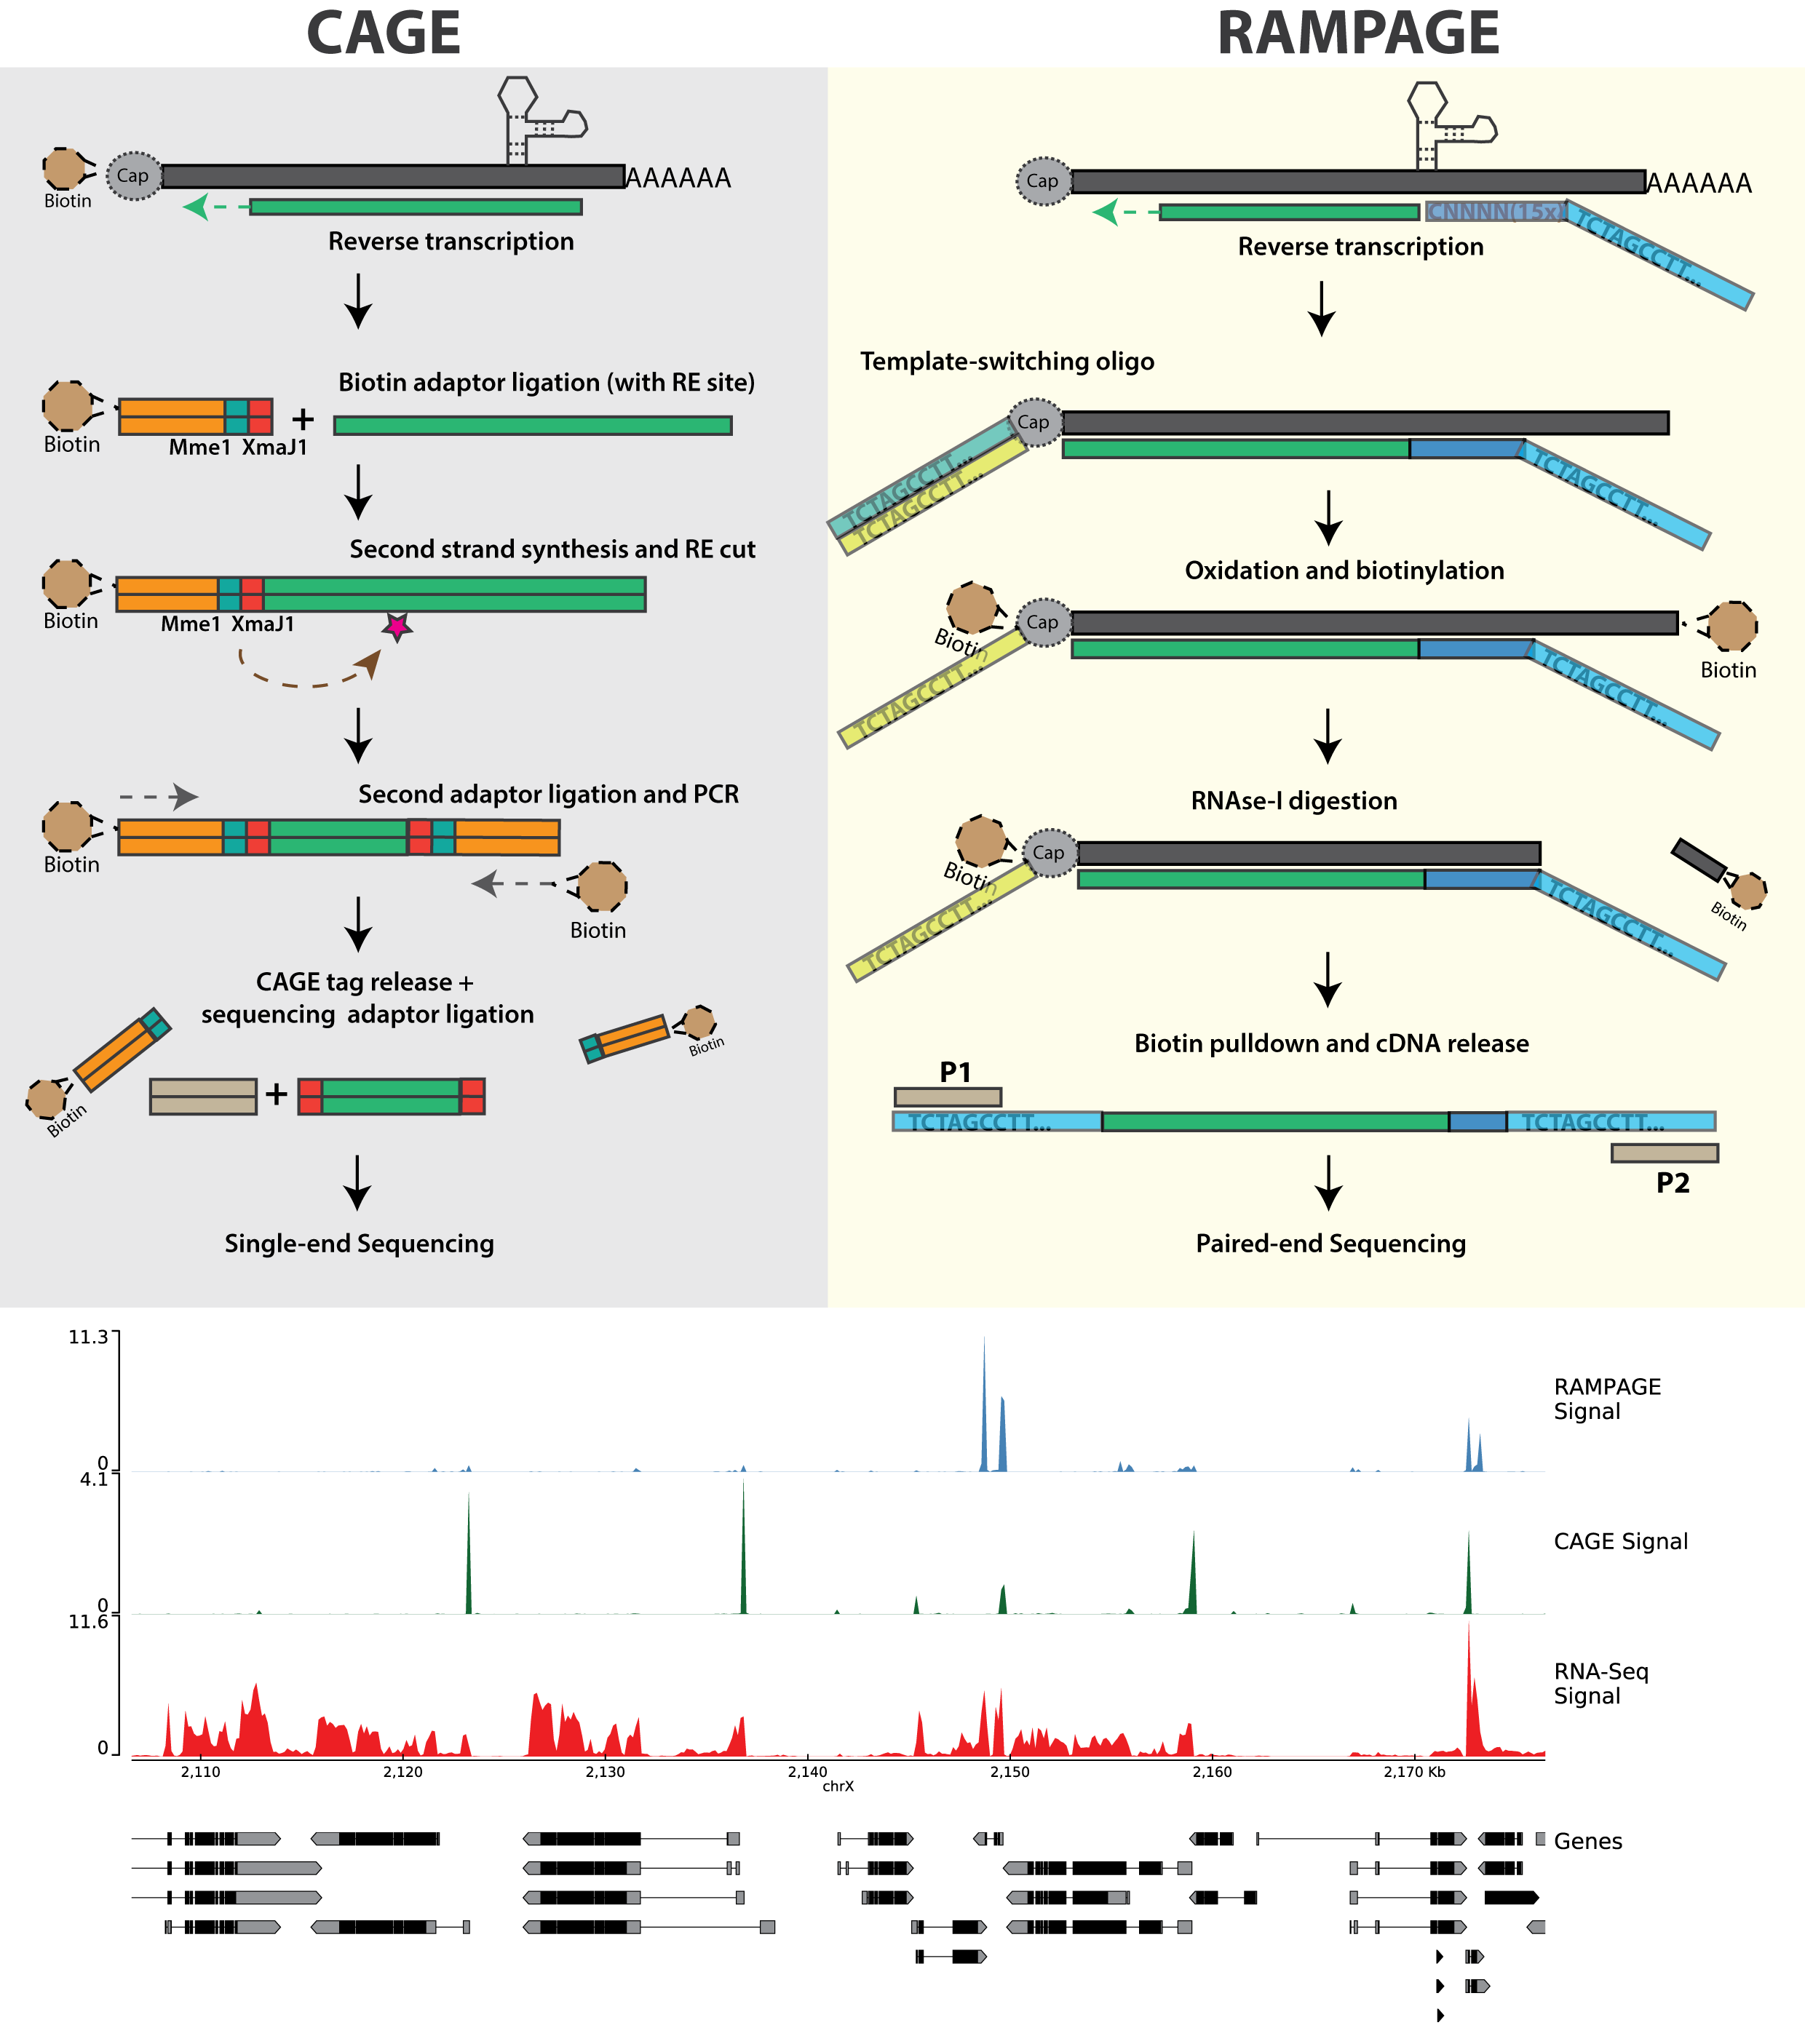
\includegraphics[width=0.8\linewidth]{figures/intro_fig5} 

}

\caption[Overview of popular promoter-profiling methods and the resulting data]{\emph{\textbf{Overview of popular promoter-profiling methods
and the resulting data.} \textbf{CAGE} begins with biotinylation and
pull-down of RNA, followed by reverse transcription and fragmentation of
cDNA using restriction enzymes (REs) to produce short (21 bp) tags.
\textbf{RAMPAGE} on the other hand, uses template-switching oligos
containing sample barcodes and PCR primers before biotinylation and
pull-down, cutting several steps from the traditional design. Both
protocols produce sharp signal at gene promoters (TSS), in contrast to
to RNA-seq (red) which produces signal all over the gene body.
Illustrations inspired by \textsuperscript{156} and
\textsuperscript{157}.}}\label{fig:unnamed-chunk-5}
\end{figure}












\clearpage

The earliest methods to identify promoters combined CAGE tags with
overlapping 5' start site into a group called \textbf{CTSS} (CAGE Tag
Start Sites), and the CTSS overlapping with each other were grouped into
\textbf{tag clusters} \textsuperscript{158}. However, this approach
(referred as ``\textbf{distclu}'') used an arbitrary cutoff to avoid
overlap between nearby tag clusters, which does not necessarily
correspond to cluster shape. Another method (referred to as
``\textbf{paraclu}''), identifies tag clusters as the segments of genome
that maximise the density of CAGE tags per nucleotide within them
\textsuperscript{159}. Clusters at various scales could be produced by
varying the minimum density (\textbf{\emph{d}}) parameter, where small
values of \emph{d} produce large, loose clusters, while large values of
\emph{d} produce small, dense clusters. The algorithm finds all clusters
for all values of \emph{d} , and therefore reports subclusters (peaks
within peaks) of TSS. Despite the improvements, the method suffers from
the issue that it does not correct for the sample-specific biases in the
protocols. Issues such as RNA composition effect and capture efficiency
of CAGE tags introduce background noise, and affect the detection of
robust, reproducible tag clusters. Another method called \textbf{reclu}
tries to filter detected clusters based on irreproducible discovery rate
(IDR) method \textsuperscript{160}. Nevertheless, methods that allow
detection of robust tag clusters by using information from biological
replicates would further improve the analysis.

\clearpage

\section{Aims}\label{aims}

The overall goal of my studies was to perform analysis and integration
of epigenomics and transcriptomics data, specifically ChIP-seq, HiC,
RNA-seq and CAGE, in order to understand the function of the
male-specific lethal (MSL) complex in flies and mammals.

In order to achieve the above goal, several bioinformatic challenges
discussed before needed to be addressed. The overall goal of the thesis
could therefore be divided into three components:
\begin{enumerate}
\def\labelenumi{\arabic{enumi}.}
\item
  Developing methods for high-resolution analysis of HiC data in order
  to understand the relationships between chromosome conformation and
  gene regulation in flies that can be applied to understand the
  mechanism of action of MSLs.
\item
  Improving existing methods of analysis of promoter profiling in order
  to perform high-resolution analysis of MSL-mediated dosage
  compensation on the X-chromosome in flies.
\item
  Finally, developing workflows for quality control, analysis and
  integration of data from multiple epigenomic assays, specifically in
  an allele-specific manner, and utilize them to understand the function
  of MSLs on the X-chromosome in mammals.
\end{enumerate}
\chapter{Results and Discussion}\label{results-and-discussion}

The following chapter summarizes the methods and insights from the six
manuscripts presented in the appendix of this thesis.

\textbf{Appendix A.1} corresponds to \textbf{Ramirez and Bhardwaj et. al
(2018)} where we perform high-resolution analysis of online HiC datasets
in flies and explore the relationship between chromosome conformation,
regulatory elements and transcription. We also introduce our tools and
resources for HiC analysis.

\textbf{Appendix A.2} corresponds to \textbf{Wolff et. al (2018)} which
describes the implementation of our HiC analysis tools into a Galaxy
web-server for end-to-end HiC analysis.

\textbf{Appendix A.3} corresponds to \textbf{Bhardwaj and Semplicio et.
al (2018)} where we introduce a new experimental protocol and analysis
software for promoter-profiling, and apply them for the analysis of
dosage compensation in flies. Experimental data for this manuscript was
generated by Giuseppe Semplicio.

\textbf{Appendix A.4} corresponds to \textbf{Aktas and Ilik et. al
(2017)} where we describe the function of mammalian ortholog of MLE
(DHX9) in controlling genome-wide RNA processing defects mediated by Alu
transposons in humans. Experimental data for this manuscript was
generated by Tugce Aktas and Ibrahim Ilik.

\textbf{Appendix A.5} corresponds to \textbf{Ramirez and Ryan et. al
(2016)} which introduces an upgrade to the previously published toolkit
from our group ``deepTools'', expanding its scope to various epigenomic
and transcriptomic assays.

\textbf{Appendix A.6} corresponds to \textbf{Bhardwaj and Heyne et. al
(2018)} which introduces ``snakePipes'', a set of scalable and flexible
pipelines that simplify integrative analysis of epigenomic data.

\section{Insights from high-resolution chromosome conformation analysis
in
flies}\label{insights-from-high-resolution-chromosome-conformation-analysis-in-flies}

A previous study from our lab investigated the conformation of the male
X-chromosome in flies in order to understand the mechanism of targeting
of the MSL complex \textsuperscript{161}. Fidel Ramirez, Thomas Lingg
and others generated HiC profiles in \emph{Drosophila} S2 cells using
the Hind-III RE, and produced HiC matrices at an average resolution of
4.5 Kb, using the Hind-III cut-sites in the genome as bins. Analyses of
this data revealed that MSL2 bound high-affinity sites cluster together
in 3D space on the X-chromosome, facilitating the spread of the MSL
complex. During the study, read filtering, matrix generation, and
normalization using the ICE method \textsuperscript{134} was implemented
by Fidel in the early version of a command line tool called HiCExplorer.

Studies published later \textsuperscript{162,163} performed HiC using
the 4-cutter Dpn-II enzyme. This data, combined with the ability of
HiCExplorer to create matrices at restriction fragment (RF) resolution,
allowed us to study the fly genome at sub-kilobase resolution
(\textasciitilde{}570 bp) and further understand the relationship
between DNA elements, chromosome conformation and transcription
\textsuperscript{164}.

\subsection{Setup of a HiC analysis
workflow}\label{setup-of-a-hic-analysis-workflow}

In order to facilitate high-resolution analysis of HiC data, we first
improved the TAD calling method described in \textsuperscript{161} (see
details in \textsuperscript{164}). Specifically, 1) The original matrix
is transformed into a z-score matrix before calculating the
TAD-separation score 2) For each bin in the genome, the TAD-separation
score is calculated for multiple window sizes around the bin and
averaged to reduce noise 3) After identification of bins with ``local
minima'' of TAD-separation scores, a Wilcoxon rank-sum test is performed
to compare the distribution of that bin with the nearby (left and right)
regions, followed by multiple testing correction.

\clearpage
\begin{figure}

{\centering 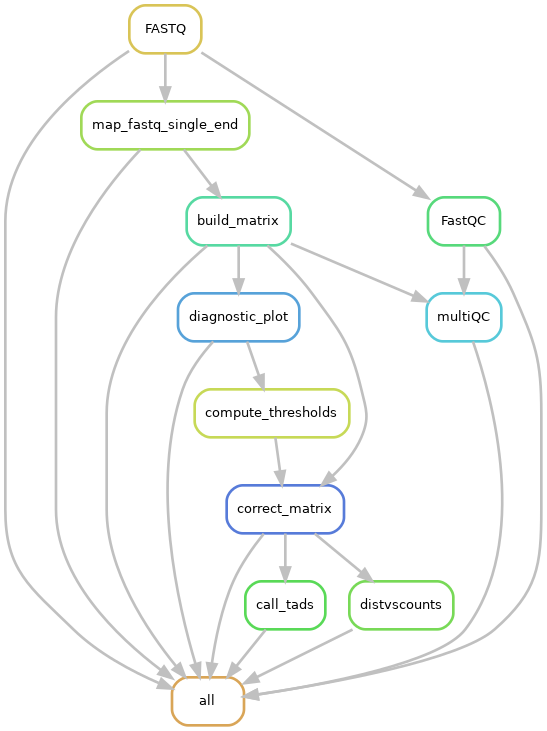
\includegraphics[width=0.5\linewidth]{figures/results_fig1} 

}

\caption[A directed acyclic graph (DAG) of the HiC workflow]{\emph{\textbf{A directed acyclic graph (DAG) of the HiC
workflow.} It includes FASTQ file quality controls (FastQC) mapping,
matrix generation, QC plots, matrix correction and TAD detection. The
step marked as ``all'' collects the final outputs. This workflow has
been implemented in snakePipes (see last section).}}\label{fig:unnamed-chunk-6}
\end{figure}






I utilized HiCExplorer to create an end-to-end HiC analysis workflow
implementing various analysis steps (see Introduction).
\textbf{Computational workflows} are like automated protocols that
perform a series of processing steps, ensuring that the dependencies
between these steps are properly resolved (for example, re-running a
5-step workflow with a missing file at step-4 re-runs both step-4 and 5
to ensure that dependent files are updated). Workflows, combined with
containerization (each step running in its own virtual environment)
ensure the transferability and reproducibility of analysis results
\textsuperscript{165}. This HiC workflow could be utilized for
reproducible analysis of both in-house and online HiC datasets (Fig 1).
The workflow is now implemented in our epigenomic analysis toolkit
called snakePipes, and is routinely used in-house for HiC data analysis.

\clearpage

\subsection{Relationships between TADs, regulatory elements, and
transcription in
flies}\label{relationships-between-tads-regulatory-elements-and-transcription-in-flies}

Using the newly implemented version of HiCExplorer tools, we detected
\textasciitilde{}2800 boundaries in wild-type female \emph{Drosophila}
Kc cells, and found that most (77\%) of the TAD boundaries in flies
associate with gene promoters. These promoter-boundaries associate with
active chromatin and have higher DNAse hypersensitivity signal (from
DHS-seq data) and stronger TAD-separation score than non-promoter
boundaries. A carefully performed DNA motif enrichment analysis
discovered that promoter-boundaries are enriched with a specific set of
core-promoter motifs : motif-1 (M1BP), 2 (Beaf32), 6, 7 (ZIPIC) and 8,
while non-promoter boundaries are enriched for some classically known
insulator motifs : CTCF, Ibf and Su(Hw). Interestingly, we find that the
motifs combinations, rather than the number of motif instances seem to
affect the strength of boundaries. Certain motifs combinations, such as
Beaf32 + Pita make the boundaries stronger while others, such as Su(Hw)
+ ibf make them weaker. Our study also challenged previous studies
showing that the number of ChIP-seq peaks of the insulator proteins
correlate with boundary strength, and rather emphasised the usefulness
of considering motifs at boundaries.

To understand whether there exists a genetic code at boundaries, we used
various classification methods, such as logistic regression, random
forest and gradient boosting models to predict boundaries using DNA
motifs. These methods performed similarly well in identifying
boundaries, with a sensitivity and specificity of over 70\% on an
independent test data. Interestingly the classifiers showed that DNAse
hypersensitivity is the most important feature in boundary prediction,
suggesting that the accessibility of DNA motifs might be a crucial
factor for boundary formation.

Using re-analysis of RNA-seq data from modENCODE, we investigated the
relationship between our high-resolution TADs and transcription. We find
that TADs serve as units of coordinated transcription during
\emph{Drosophila} development. Expression of genes with TADs are highly
correlated throughout development while genes separated by TAD
boundaries show a lack of correlation. We also find that genes at TAD
boundaries have expression features of housekeeping genes (high,
constitutive expression with low variability) which confirmed previous
studies linking housekeeping genes to TAD boundaries.
\begin{figure}

{\centering 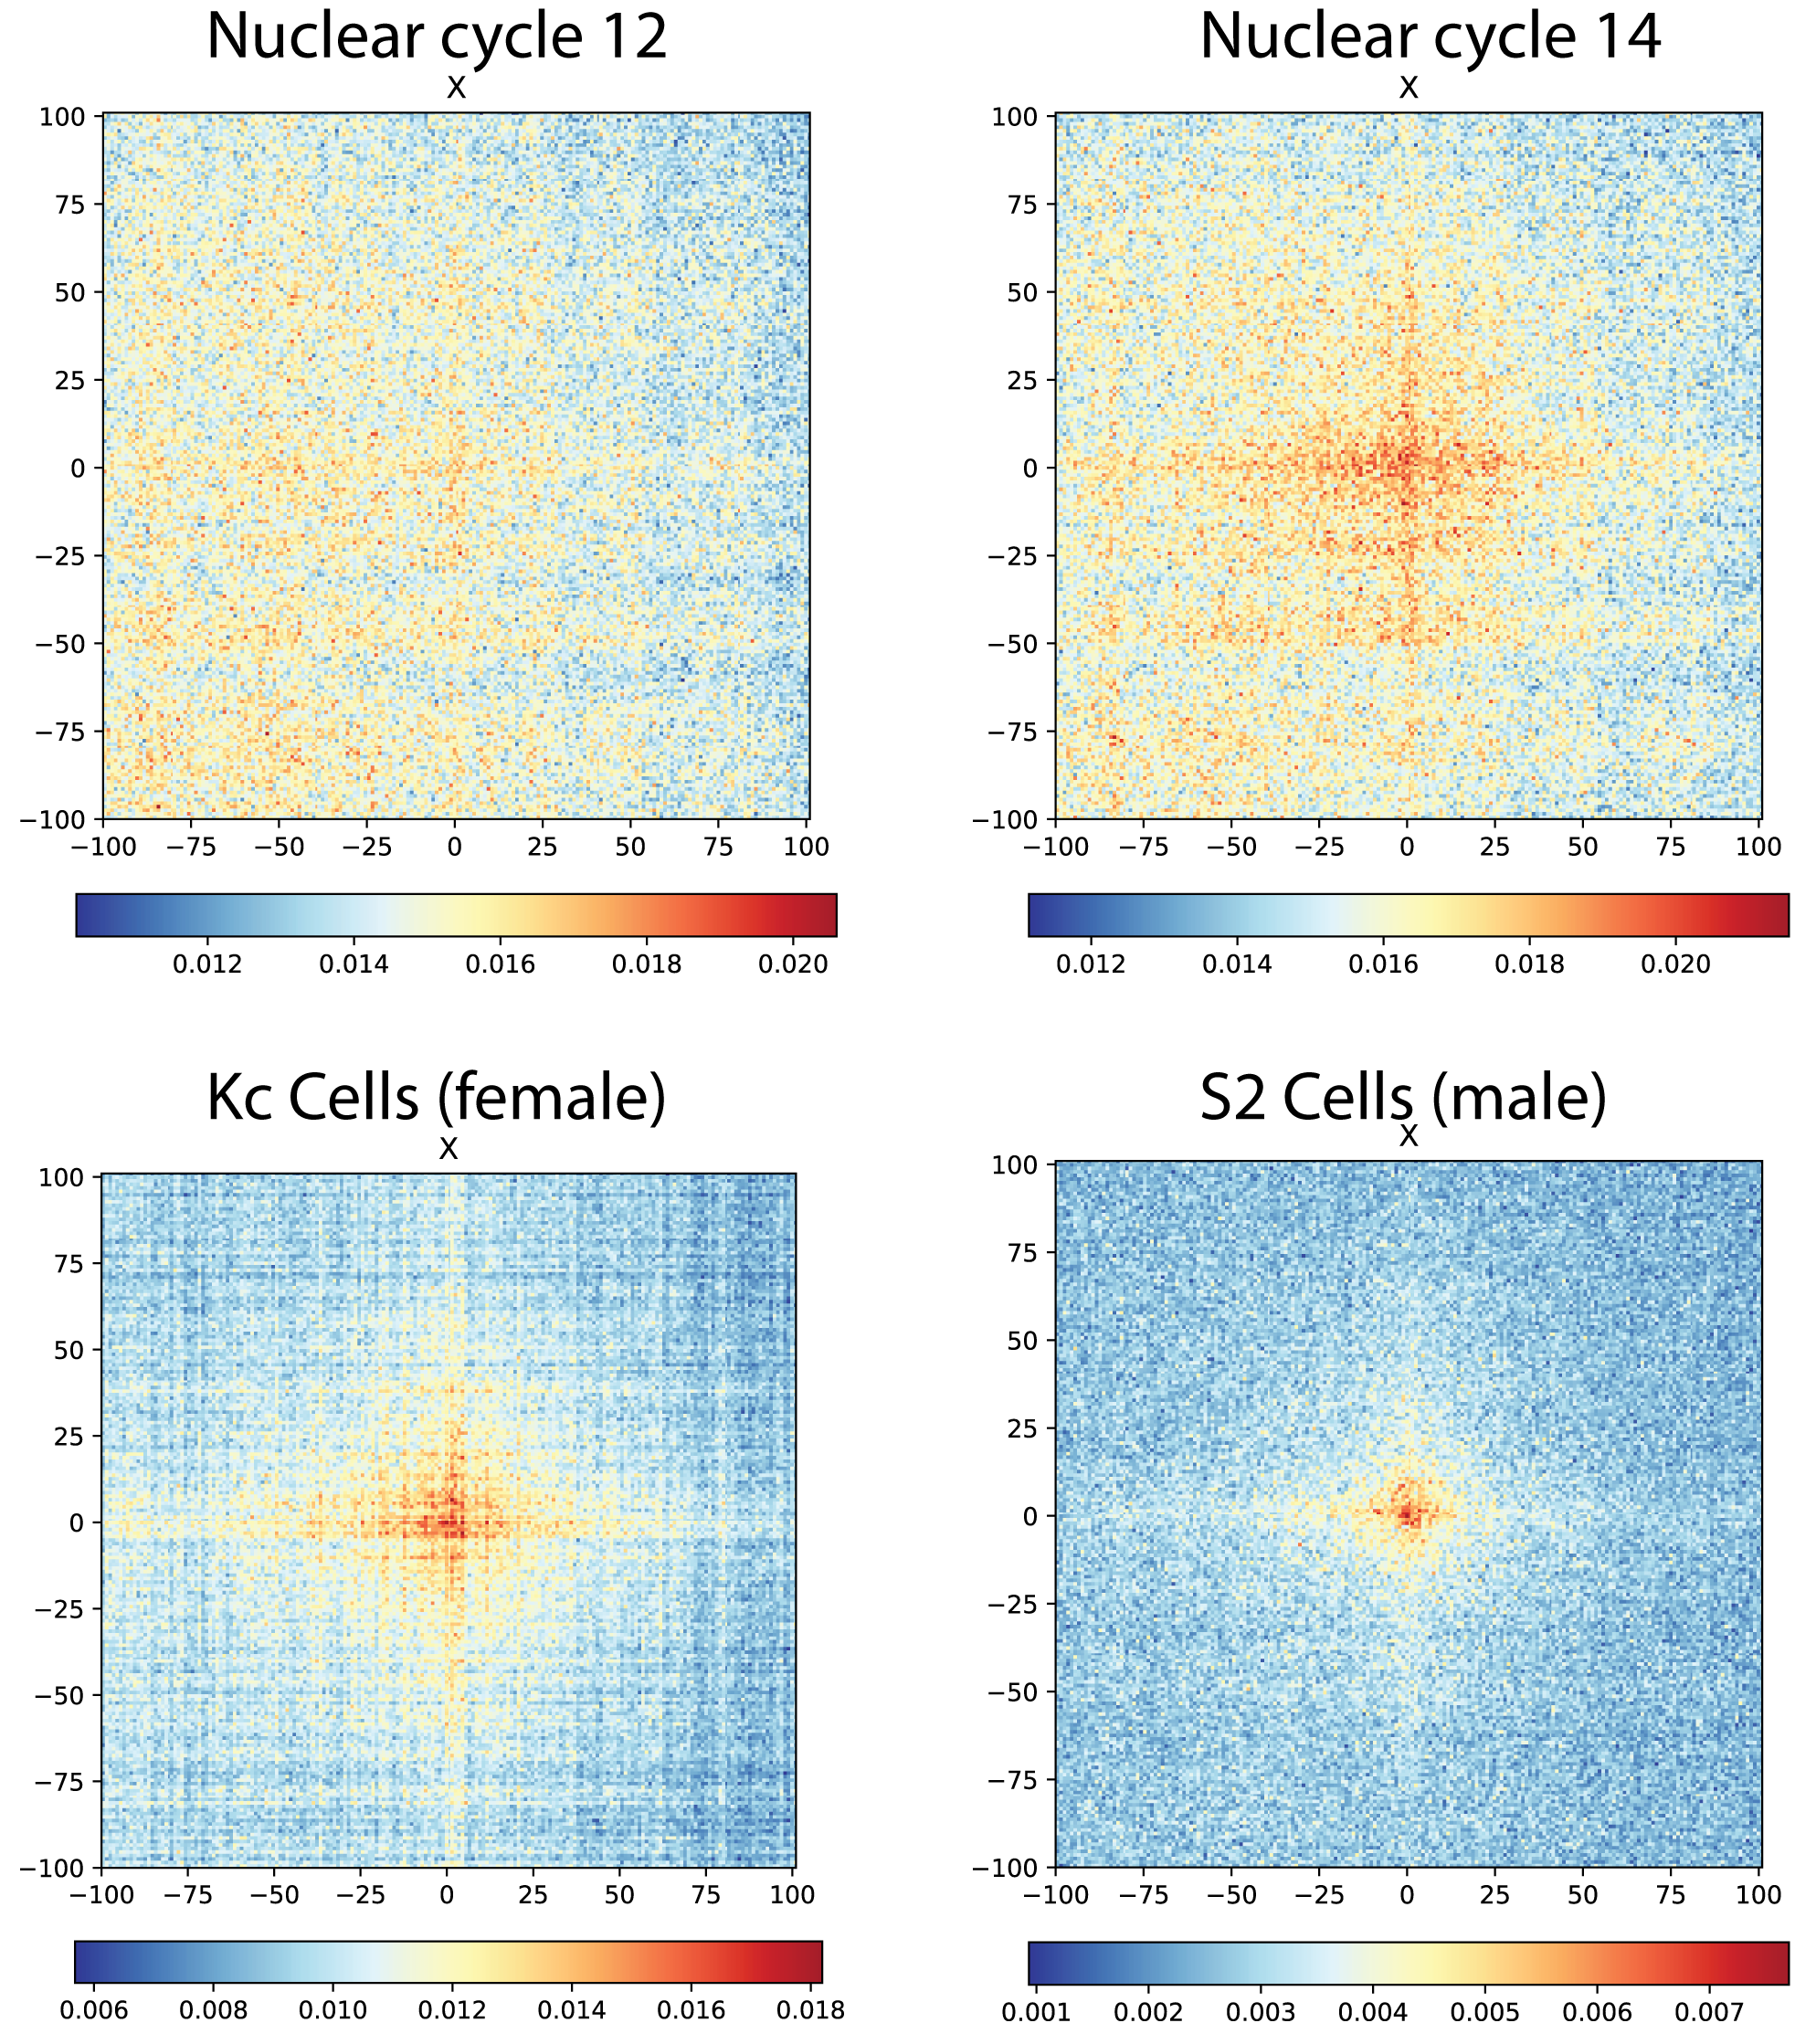
\includegraphics[width=0.7\linewidth]{figures/results_fig2} 

}

\caption[The HAS interaction network on X-chromosome]{\emph{\textbf{The HAS interaction network on X-chromosome.}
An aggregate contact matrix containing mean interactions over all
possible contacts within a genomic distance of 0.5 Mb to 15 Mb of HAS
loci. Submatrices were extracted for each HAS from the corrected HiC
matrix, and the counts were further normalized to total counts of each
submatrix. The data from multiple recent in situ HiC studies
\textsuperscript{47,162--164}, analyzed during our study.}}\label{fig:unnamed-chunk-7}
\end{figure}








The catalogue of high-resolution boundaries generated in this study
functions as useful resource in understanding the biology of MSLs, as
well as other protein complexes in context of 3D chromatin. For example,
chromator, a member of MOF-associated NSL (non-specific lethal) complex
was found to be associated with various motifs at boundaries (Fig. S3I
of \textsuperscript{164}). Further the data produced and analysed during
our study allowed us to re-evaluate our previous finding whether the
high-affinity sites cluster in 3D space. Using clustering of contact
aggregates from the data, we observed that the HAS-HAS clusters emerge
after zygotic genome activation (at nuclear cycle 14, together with the
establishment of TADs) when MSL2 expression begins
\textsuperscript{166}. Similar to \textsuperscript{161}, HAS-HAS
clusters were observed in both male and female cells, suggesting that
the MSL complex could utilize the pre-existing 3D conformation of the
X-chromosome for spreading.
\begin{figure}

{\centering 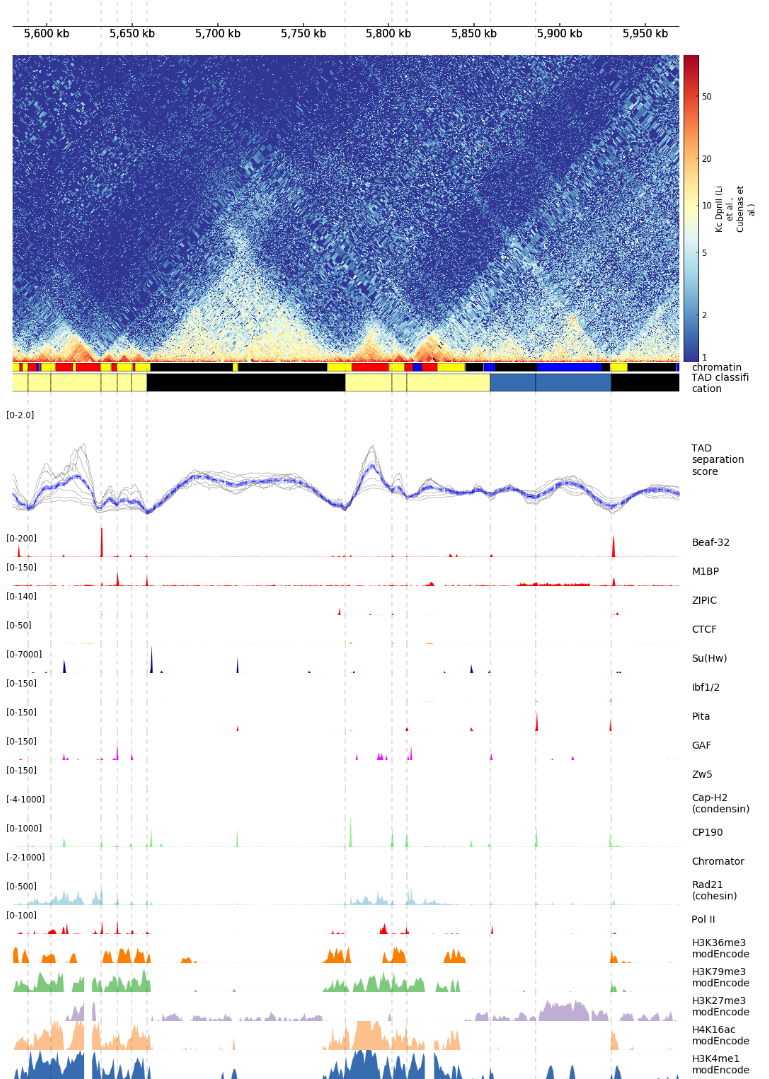
\includegraphics[width=0.8\linewidth,height=0.6\textheight]{figures/results_fig3} 

}

\caption[Chorogenome navigator]{\textbf{Chorogenome navigator.} Snapshot of a
\textasciitilde{}350kb region around MOF in \emph{Drosophila} Kc cells,
from the chorogenome navigator web server.*}\label{fig:unnamed-chunk-8}
\end{figure}




\subsection{Resources for HiC analysis and
visualization}\label{resources-for-hic-analysis-and-visualization}

During our analysis of chromosome conformation in flies, we improved on
the methods developed and presented in the last study from our lab
\textsuperscript{161}. Fidel and I added further functionality to
HiCExplorer, such as improved TAD calling, a method to import and export
multiple file formats, and plotting methods. In collaboration with Jose
Villaveces (MPI-Biochem), we developed the visualization tool
HiCBrowser, which can be used as a standalone tool to browse HiC and
other genomic data (ChIP-seq, RNA-seq etc.). In order to allow
biologists to investigate their own gene or region of interest in
context of TADs, we developed a web server that contains online HiC data
pre-processed using our HiC workflow, along with other genomic data
({[}{\url{http:://chorogenome.ie-freiburg.mpg.de}}{]}). Further in
collaboration with Joachim Wolff and Bjoern Gruening, we implemented
HiCExplorer along with other tools in galaxy, that facilitates GUI-based
end-to-end analysis of HiC data for biologists \textsuperscript{167}. We
hope that these resources would facilitate easy and user-friendly HiC
analysis for biologists.

\section{Using promoter-profiling to study MSL-mediated dosage
compensation in
flies}\label{using-promoter-profiling-to-study-msl-mediated-dosage-compensation-in-flies}

\subsection{Development of the MAPCap
protocol}\label{development-of-the-mapcap-protocol}

In flies, we wanted to understand how MSL mediated dosage compensation
works at the level of individual transcription start sites (TSSs),
through promoter-profiling. In collaboration with Giuseppe Semplicio, I
contributed to the development of a new experimental protocol for
promoter-profiling, termed as MAPCap (\textbf{M}ultiplexed
\textbf{A}ffinity \textbf{P}urification of \textbf{Cap}ped RNA). MAPCap
is performed differently compared to the standard CAGE protocol, in the
following major ways :
\begin{enumerate}
\def\labelenumi{\arabic{enumi}.}
\item
  Instead of biotinylation of the 5-mG Cap, MAPCap performs an 5-mG
  antibody based pull-down of the transcripts.
\item
  Instead of fragmentation using a restriction site inserted during
  RT-PCR in CAGE, MAPCap utilizes sonication.
\item
  RNA is attached to an oligo containing multiplexing barcodes, random
  barcodes (as UMIs) and sequencing adaptors, allowing us to pool the
  samples early in the protocol.
\end{enumerate}
\clearpage
\begin{figure}

{\centering 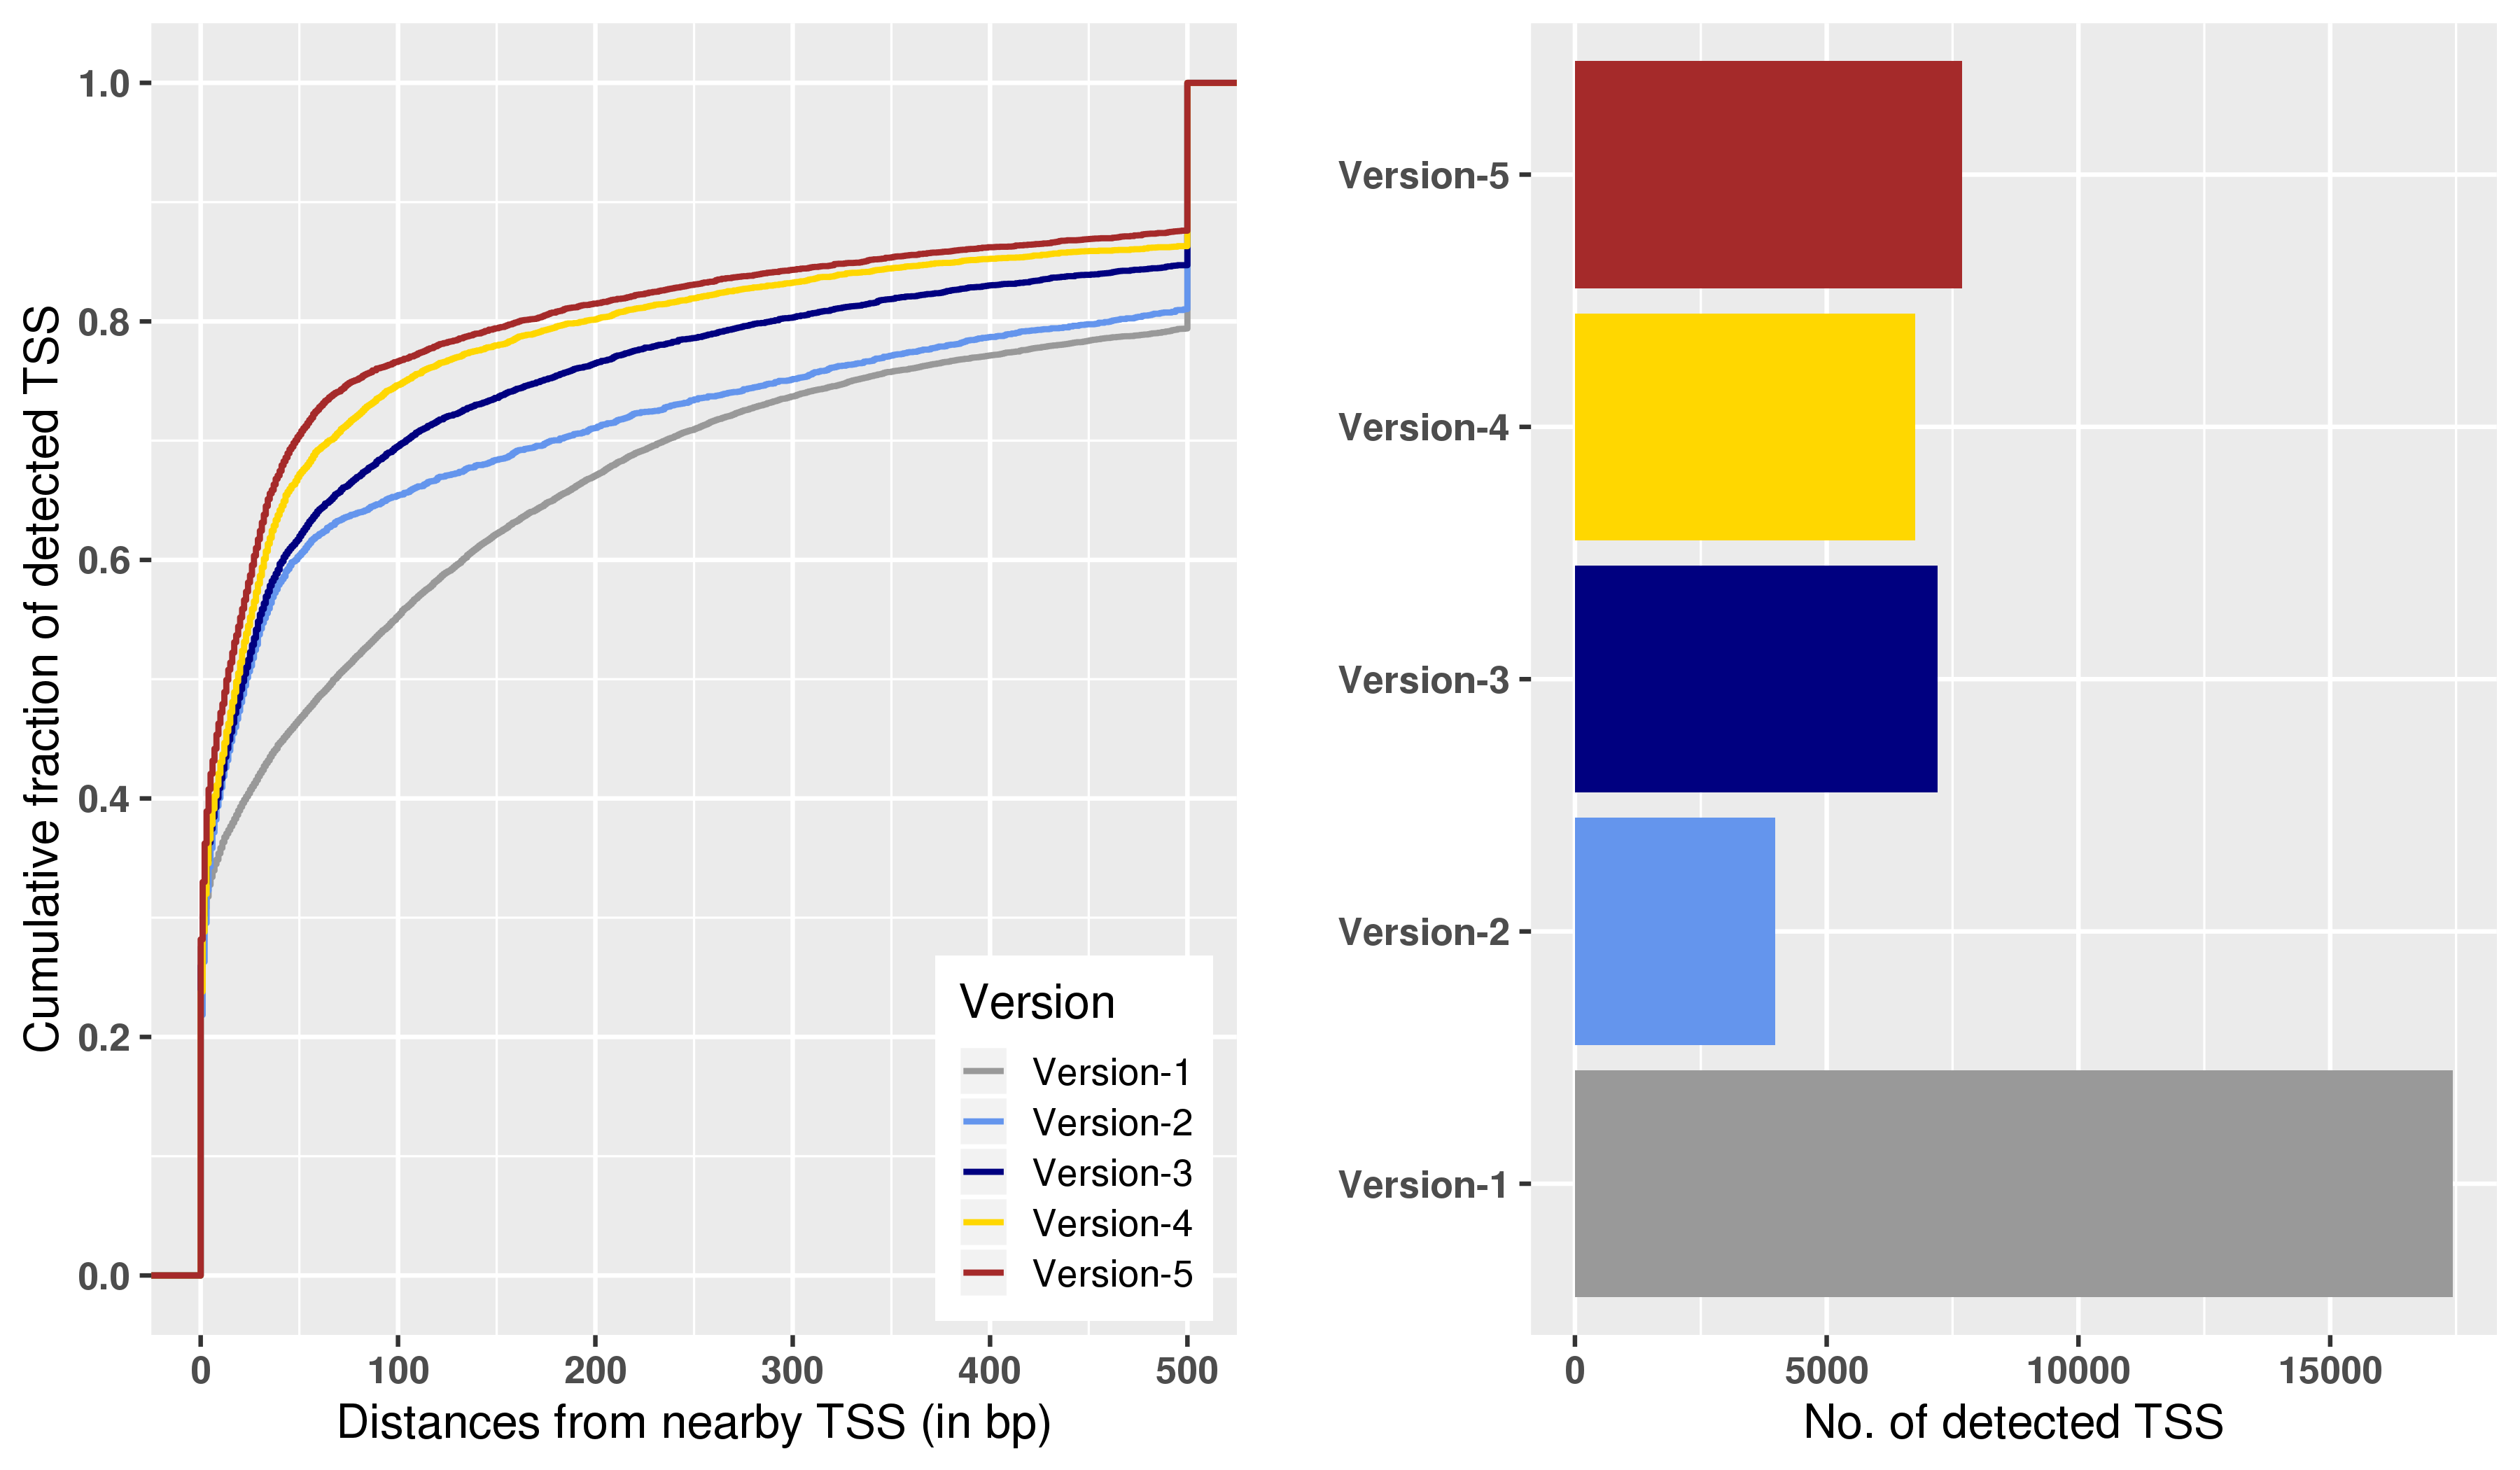
\includegraphics[width=0.9\linewidth]{figures/results_fig4} 

}

\caption[Improvement in TSS detection over different versions of the MAPCap protocol]{\emph{\textbf{Improvement in TSS detection over different
versions of the MAPCap protocol} (not completely in chronological
order). \textbf{Left :}} \emph{Distance} \emph{of detected TSS to an
annotated TSS. As the protocol improved, the detected TSSs became closer
to the annotated TSSs in the genome. \textbf{Right :} Number of detected
TSSs for each version. Version 1 has the highest number of detected
TSSs, however the precision plot shows that it was mostly due to low
signal-to-noise ratio. The number of detected TSSs remains constant for
the later versions of the protocol while the precision improved. All
samples utilized 5ug of RNA, and TSSs were detected in all samples using
the ``distclu'' method with identical parameters. }}\label{fig:unnamed-chunk-9}
\end{figure}












Development of the MAPCap protocol required multiple rounds of
optimizations, where the fragmentation, handling of abundant RNAs,
reverse-transcription, and sample multiplexing strategies were changed
in response to the insights from the data analysis. \emph{Figure 3.4}
shows how the TSS detection has improved over the various versions of
the protocol.

An important insight from the development of the protocol has been the
effect of RNA composition bias on the final analysis. In case of
protocols like MAPCap, that allow early multiplexing, the effect of
composition bias is more pronounced, since there are multiple steps
where high abundance RNA can ``take over'' the overall library
composition. Promoter-profiling is usually performed on ribo-depleted
RNA, and the RNA composition fluctuates for each run, especially for
samples derived from tissues \emph{(Fig. 3.5)}. This emphasised the need
of the methods to account for composition bias (such as TMM
\textsuperscript{168}), and the usefulness of replicates in the
detection of robust TSSs in presence of noise.
\begin{figure}

{\centering 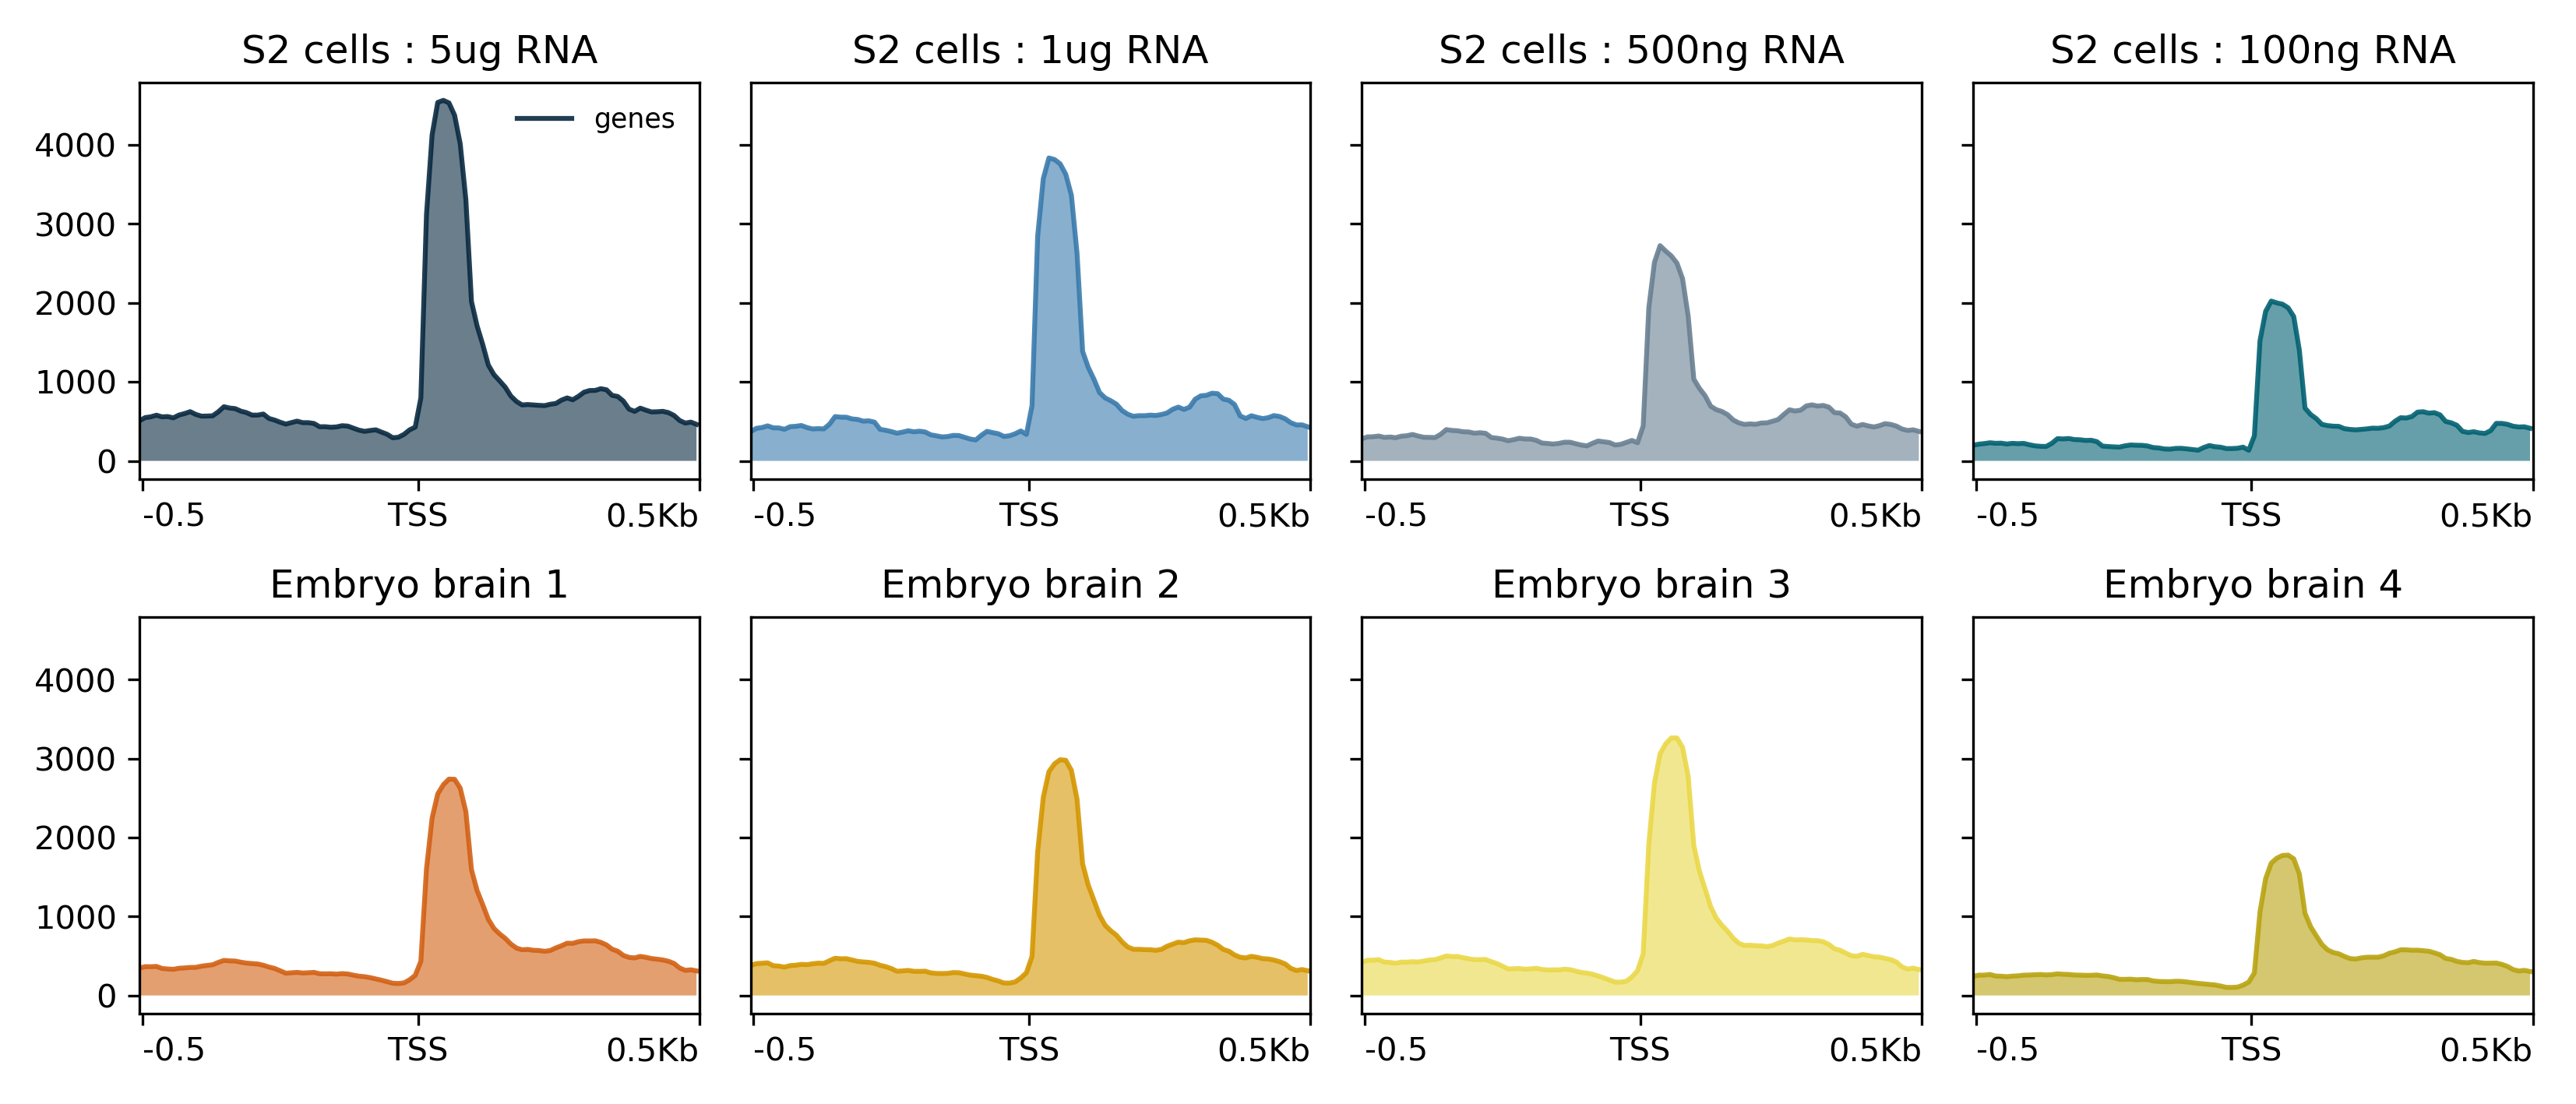
\includegraphics[width=0.9\linewidth]{figures/results_fig5} 

}

\caption[Effect of RNA composition on TSS enrichment]{\emph{\textbf{Effect of RNA composition on TSS enrichment}
(RPKM normalized signal on TSS). \textbf{Upper} panel shows the data
from a MAPCap run where different input concentrations of RNA were
multiplexed. Enrichment decreases as the amount of input RNA gets lower.
\textbf{Lower} panel shows data from a MAPCap run where total RNA was
extracted from different embryos brains. The concentration varies
between 200-500 ng per sample. Lower panel represents a more practical
MAPCap run, since the RNA composition couldn't be precisely controlled.}}\label{fig:unnamed-chunk-10}
\end{figure}









\subsection{Development of the icetea bioconductor
package}\label{development-of-the-icetea-bioconductor-package}

The new generation promoter-profiling protocols such as MAPCap, and the
recently introduced RAMPAGE \textsuperscript{157} protocol demand a set
of data processing steps different from traditional CAGE. The raw FASTQ
files obtained from the protocol contain sample multiplexing barcodes,
which are used to separate the samples, and the random barcodes, which
could be used to remove PCR duplicates during the analysis. The
paired-end data produced by this protocol could be used to improve
mapping and annotation of peaks. Also, multiplexing makes it easier for
biologists to include biological replicates in their experiments, which
could be useful in performing robust TSS detection and downstream
analysis (see introduction). Also, a good correlation between expression
estimates between MAPCap and RNA-seq suggested that after appropriate
normalization, a MAPCap experiment with biological replicates could also
be used for differential TSS expression analysis.

Keeping the above observations in mind, I created a user-friendly R
package called \textbf{icetea} (\textbf{I}ntegrating \textbf{C}ap
\textbf{E}nrichment and \textbf{T}ranscript \textbf{E}xpression
\textbf{A}nalysis) that performs processing, TSS detection and
differential expression analysis from data such as those from MAPCap and
RAMPAGE. \textbf{icetea} implements a new TSS detection approach based
on ``local enrichment'' of CAGE tags, that's inspired from ChIP-seq
analysis. It uses replicates to model robust fold-changes of genomic
windows with respect to their local background, and a user-specified
fold-change cutoff is used to detect TSS. Further, \textbf{icetea} can
be used to perform various internal (TMM, RLE etc.) or external
(spike-in) normalization of data and detect differentially expressed
TSSs between two conditions. \textbf{Icetea} is available for use from
bioconductor ({[}{\url{https://bioconductor.org/packages/icetea}}{]}).

\subsection{Transcriptional changes during dosage compensation defects
in
flies}\label{transcriptional-changes-during-dosage-compensation-defects-in-flies}

In order to gain insights into transcript-specific dosage compensation
in flies, we performed MAPCap, together with RNA-seq, on brains
extracted from male and female fly larvae. RNAs were extracted from the
mutants of the \emph{maleless} (MLE) gene, which is required for the
targeting of the MSL complex to X-chromosome through recognition of roX
RNAs. Therefore, mutant males are expected to have defects in the
upregulation of the X-chromosome. We then deployed a processing pipeline
based on icetea for the analysis
({[}{\url{https://github.com/vivekbhr/cage/_pipeline}}{]}). Analysis
showed that most promoters are similarly used between male and female
flies. MLE KO leads to a downregulation of majority of TSSs on the
X-chromosome in males ( \textgreater{}1700 downregulated TSSs), but have
almost no effect on females (\textasciitilde{}23 TSSs differentially
expressed). Very few (241) upregulated TSS were observed genome-wide,
with only 14 on X-chromosome. Analysis of wild-type ChIP-seq data on the
differentially expressed TSSs showed that both the downregulated and
unchanged TSSs had similarly high H4K16ac levels which, while the
upregulated TSSs showed low H4K16ac levels in both sexes. We are further
generating H4K16ac ChIP-seq in MLE KO to investigate the TSS which
remain unchanged upon MLE KO in the MAPCap data in order to understand
whether their resistance to change in promoter usage is dependent on
their H4K16ac levels.

\clearpage
\begin{figure}

{\centering \includegraphics[width=0.9\linewidth]{figures/results_fig6} 

}

\caption[TSS expression (MAPCap) and H4K16ac levels (ChIP-seq) on male and female embryo brains]{\emph{\textbf{TSS expression (MAPCap) and H4K16ac levels
(ChIP-seq) on male and female embryo brains.} Upon KO of MLE, male
brains show about \textasciitilde{}2-fold downregulation, while female
brains do not show a large change. Both downregulated and unchanged TSS
have similar H4K16ac levels in wild-type cells (males have higher level
than females on the X). The plot is made using an new version of
deepTools \textsuperscript{120} that allow creation of coverage files
and visualization of data from multiple assays together.}}\label{fig:unnamed-chunk-11}
\end{figure}









\section{Integrating transcriptomic and epigenomic analysis to study
MSLs in
mammals}\label{integrating-transcriptomic-and-epigenomic-analysis-to-study-msls-in-mammals}

\subsection{The role of MSL complex member MLE in
mammals}\label{the-role-of-msl-complex-member-mle-in-mammals}

All MSL complex members, except the roX RNAs, are conserved from
\emph{Drosophila} to mammals (see introduction) and previous study from
our lab based on ChIP-seq of the MSLs discovered their genome-wide
localization on gene promoters and enhancers \textsuperscript{96}. The
role of the conserved homolog of MLE, termed as DHX9, was however not
investigated in this study. To study the functions of the DHX9 RNA
helicase, Tugce Aktas and Ibrahim Ilik in the lab performed an improved
version of RNA-CLIP : a method used to determine RNA binding partners of
a protein of interest. This method, termed UV-CLAP (Ultraviolet Cross
Linking and Immunoprecipitation) produced a genome-wide map of DHX9-RNA
interactions, and the visual inspection of the data revealed that DHX9
seems to preferentially bind to human Alu elements in the genome.

In collaboration with Tugce and Ibrahim, I performed a genome-wide
enrichment analysis of various Alu subfamilies in the DHX9 UV-CLAP data
using two independent approaches : 1) consensus repeat mapping, followed
by enrichment analysis (adopted from \textsuperscript{169}) and 2)
graph-based clustering of raw DHX9 bound sequences (adopted from
\textsuperscript{170}). Both approaches revealed a significant
association of DHX9 with Alu repeats in humans, and their evolutionary
relatives : B1 transposons in mice. DHX9 was preferentially enriched on
young AluS and AluY families enriched in gene introns. To further
investigate the role of DHX9-Alu interaction at the introns, Ibrahim
performed RNA-seq experiment with poly-A selected and poly-A depleted
RNA. My analysis of this data revealed that DHX9 depletion leads to
widespread defects in gene expression and splicing, and an increase in
production of circular RNA species in the cell. Further, since intronic
Alu elements are frequently associated with RNA editing
\textsuperscript{171--174}, I developed a workflow for detection of RNA
editing from the RNA-seq data
({[}{\url{https://github.com/vivekbhr/dhx-alu}}{]}). Using the workflow,
we identified both an increase and decrease of RNA editing genome-wide,
although RNA editing explained only a minor fraction of gene expression
changes. Overall, this analysis revealed for the first time that DHX9
has a major role in regulating RNA processing defects contributed by the
Alu elements in the human genome \textsuperscript{175}.

\subsection{The role of MSL complex on active and inactive mammalian
X-chromosomes}\label{the-role-of-msl-complex-on-active-and-inactive-mammalian-x-chromosomes}

Probing the function of the MSL complex in mammals, the previous study
from our lab discovered that the differentiation of female mouse
embryonic stem cells (ESCs) depleted for MSL complex members (MSL1 and
MSL2) leads to chaotic inactivation of the X-chromosome. A fraction of
these differentiating neural progenitor cells (NPCs) showed both X
chromosomes being inactivated \textsuperscript{96}. This effect of MSLs
was attributed to their regulation of the Tsix promoter through H4K16ac.
In order to further investigate the function of MSLs on the
X-chromosome, we sought to 1) generate genome-wide binding profiles of
MSLs in female mouse cell lines 2) Investigate the effect of MSL loss in
a system independent of Tsix effects.

Tomsaz Chelmicki therefore generated ChIP-seq profiles of MSLs in female
ESCs and NPCs derived from a mouse strain of hybrid origin, a cross
between \emph{Mus musculus} (strain 129Sv) and \emph{Mus castanious}
(Cast) \textsuperscript{176}. To study effects independent of Tsix, Raed
Hmadi generated KOs for MSL2 in the NPCs, where X-inactivation has
already been established. We then generated RNA-seq profiles of these KO
clones, along with the wild-type controls. Further, in collaboration
with Laura Arrigoni and Ralf Gilsbach, we generated profiles of various
histone marks using RELACS \textsuperscript{177}, open chromatin
profiles using ATAC-seq \textsuperscript{178}, and whole genome
methylation profile using bisulfite-seq (WGBS) \textsuperscript{179} on
wild-type and KO NPCs.

For analysis of these datasets we needed an approach of mapping and
sorting of genomic alignments in an allele-specific manner. I utilized
an approach that masks the positions of single nucleotide polymorphisms
(SNPs) coming from parental strains in the reference genome before
mapping, followed by sorting of unique allele-specific alignments. This
method, implemented in the tool SNPsplit \textsuperscript{180},
overcomes the ``reference bias'' : an issue that reads coming from a
strain that's genetically closer to the reference genome, would map
better to the reference genome in absence of SNP masking
\textsuperscript{181}. Workflows for analysis of epigenomic data that
could perform allele-specific sorting were developed (see next section)
and applied for the analysis of MSL2 KOs.
\begin{figure}

{\centering 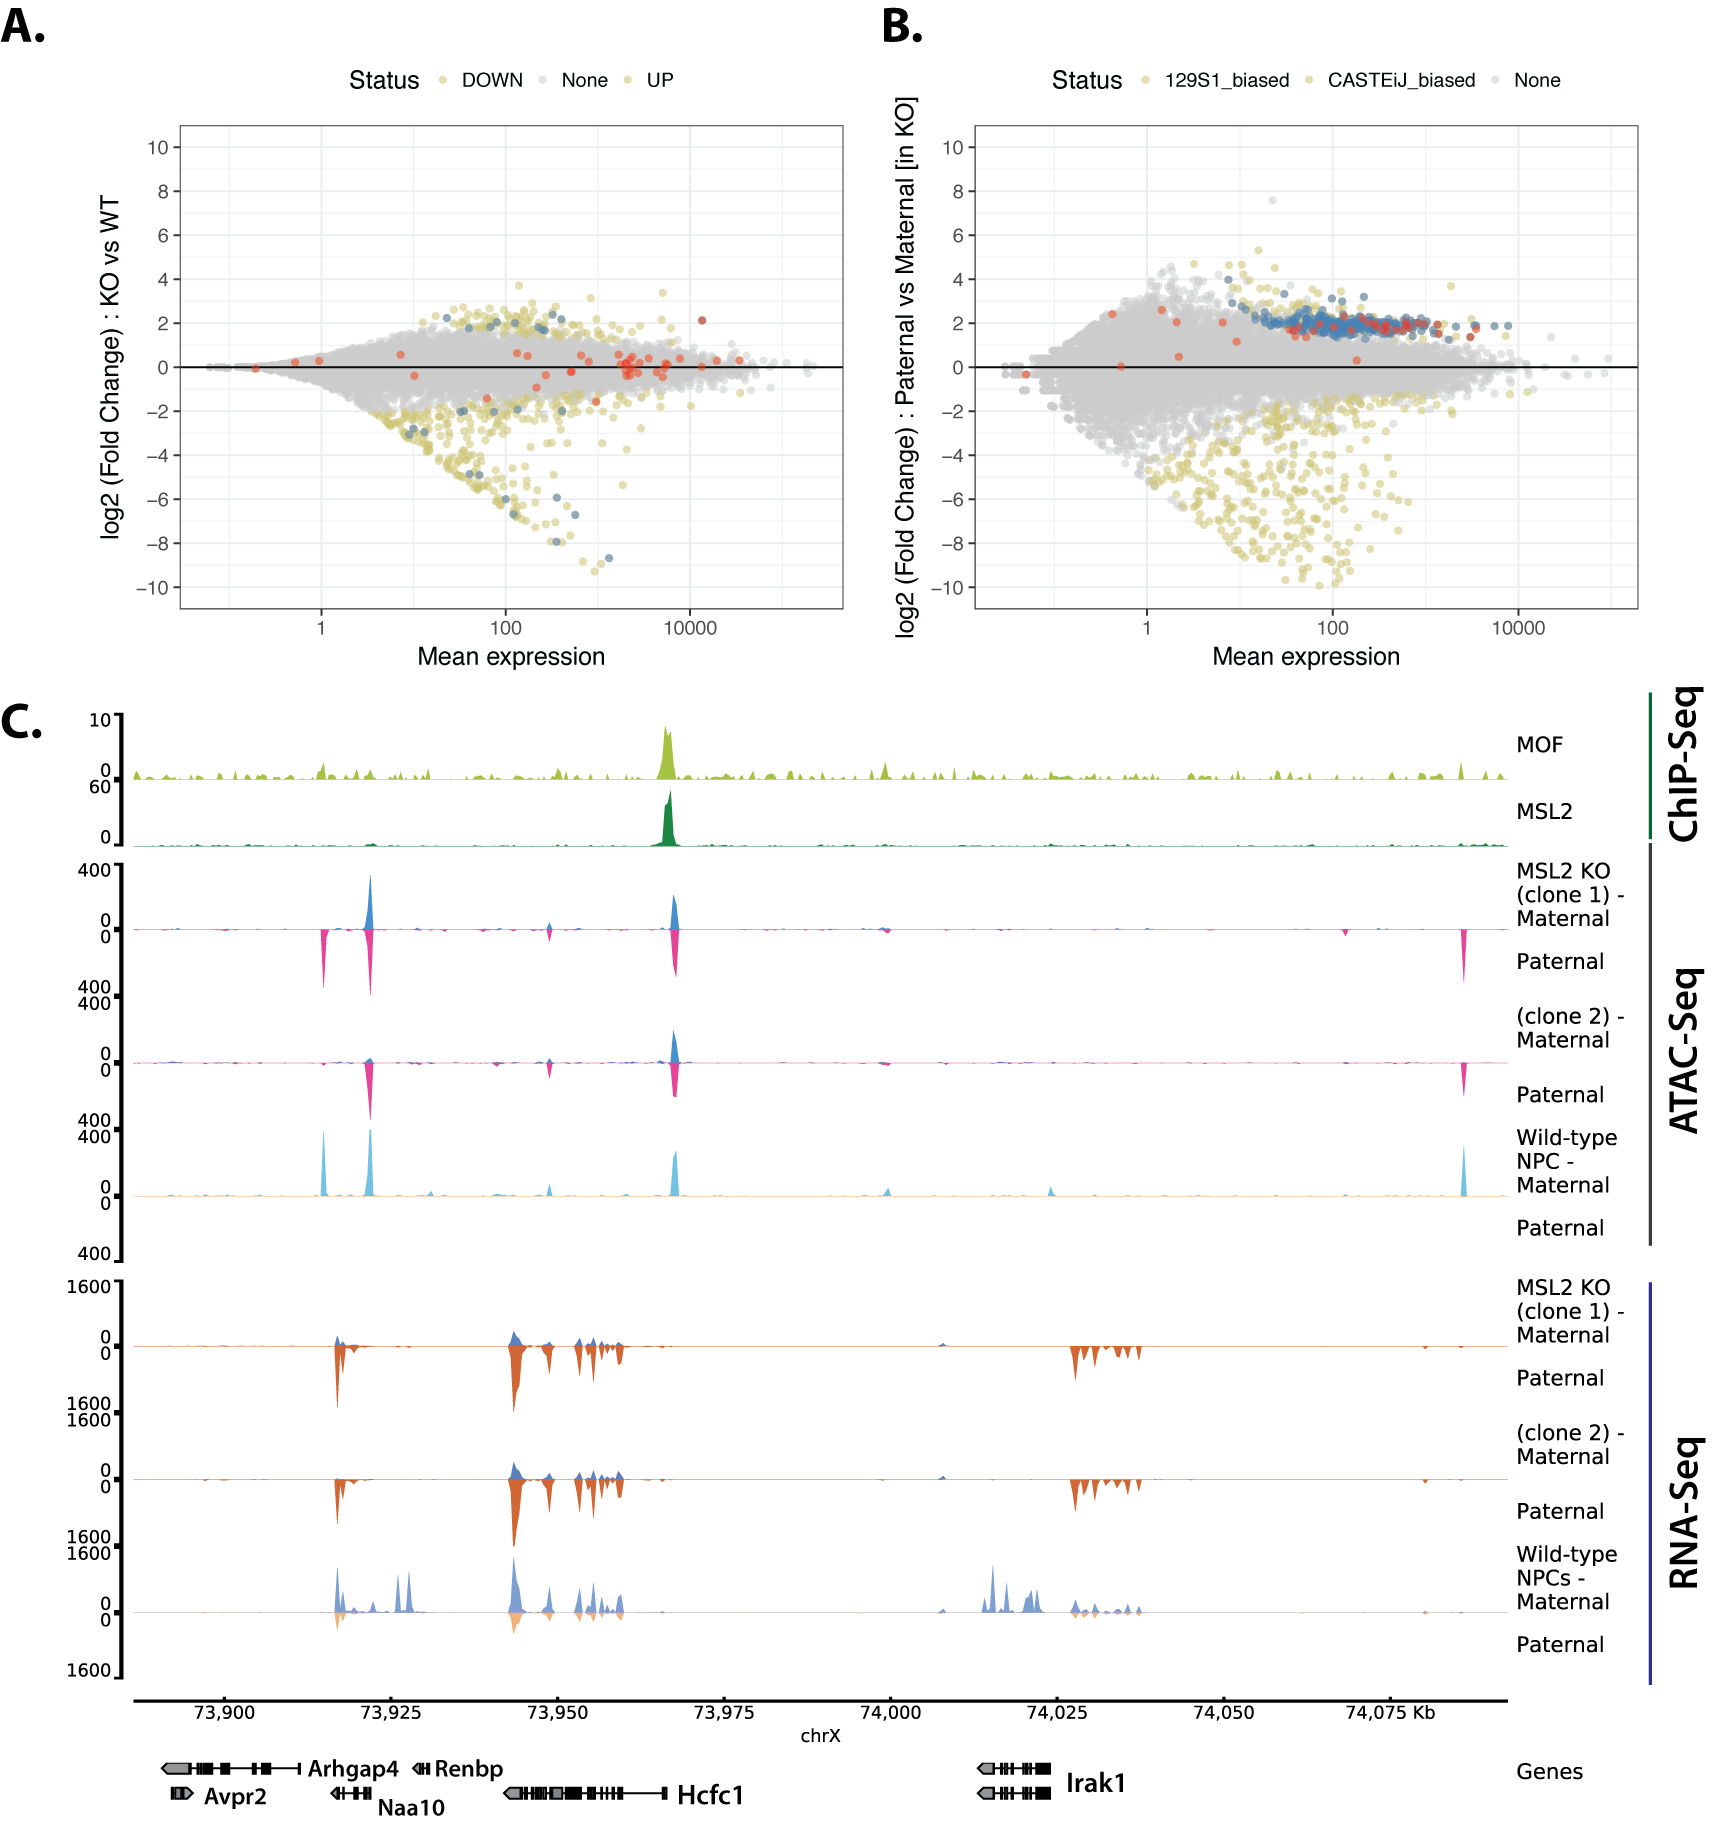
\includegraphics[width=1\linewidth,height=0.7\textheight]{figures/results_fig7} 

}

\caption[Integrative analysis of ChIP-seq, RNA-seq and ATAC-Seq in MSL2 knockout (KO) NPCs]{\emph{\textbf{Integrative analysis of ChIP-seq, RNA-seq and
ATAC-Seq in MSL2 knockout (KO) NPCs.} \textbf{A)} The MSL2 bound genes
on X-chromosome (marked in red) seem to be unaffected in normal RNA-seq
analysis. Genes differentially expressed between KO and Wild-type cells
are marked in green, and affected genes on chrX are marked in blue
\textbf{B)} Allele-specific analysis of the data reveals that genes on
the X show a clear bias in expression towards the paternal allele
(blue). Many of these genes are bound by MSL2 at their promoters (red).
\textbf{C)} Genome browser track showing a locus with escapees of Xi,
MSL2 KO shows activation of paternal allele expression, concordant with
open chromatin changes.}}\label{fig:unnamed-chunk-12}
\end{figure}












\clearpage

Applying our analysis workflow to MSL2 ChIP-seq data revealed that
after, but not before differentiation into NPCs, MSL2 binds to
significantly more loci on the inactive X-chromosome (Xi), compared to
the active X (Xa). Analysis of RNA-seq data revealed an allele-specific
downregulation of genes associated with MSL2 binding, upon the loss of
MSL2. However the loss on one allele-was compensated by a gain in
expression from another allele. Analysis of ATAC-seq data in the KOs
suggested that this effect is transcriptional, since the promoters
associated with loss of expression show a loss of open chromatin and
vice-versa \emph{(Fig. 3.7)}. This analysis suggests that MSL2 might be
important for maintaining the allelic balance in expression of their
target genes. Further, there seems to be an allelic-sensing mechanism on
the chromosome that compensates for the loss of MSL2 on the target
allele. Further integrative analysis of this data to understand the
effects of MSLs on the X-chromosome is underway.

\subsection{A toolkit for integrative epigenomic
analysis}\label{a-toolkit-for-integrative-epigenomic-analysis}

The analysis of various epigenomic datasets described in the section
above is a massive challenge for a single bioinformatician, and demands
a set of uniform processing pipelines. We sought to develop a pipeline
that would also allow flexible processing of datasets such that future
users are able to change parameters and perform exploratory analysis.
This pipeline should be scalable, to run hundreds to thousands of jobs
at once, and should be easy to install and use in future. I joined the
existing efforts by Steffen Heyne and others in the bioinformatics unit
to develop a toolkit that allows analysis of ChIP-seq, RNA-seq,
ATAC-seq, WGBS, HiC and single cell RNA-seq data. This toolkit, called
\textbf{snakePipes}, implements various methods and workflows described
in the previous sections, in a user-friendly command-line interface. The
pipeline also performs allele-specific analysis of data as described in
the previous section, upto the point of downstream analysis, such as
differential expression, or differential peak detection. With
snakePipes, we hope that biologists would be able to easily replicate
the results from ours and other published studies that present multiple
epigenomic assays \textsuperscript{182}.

\clearpage
\begin{figure}

{\centering 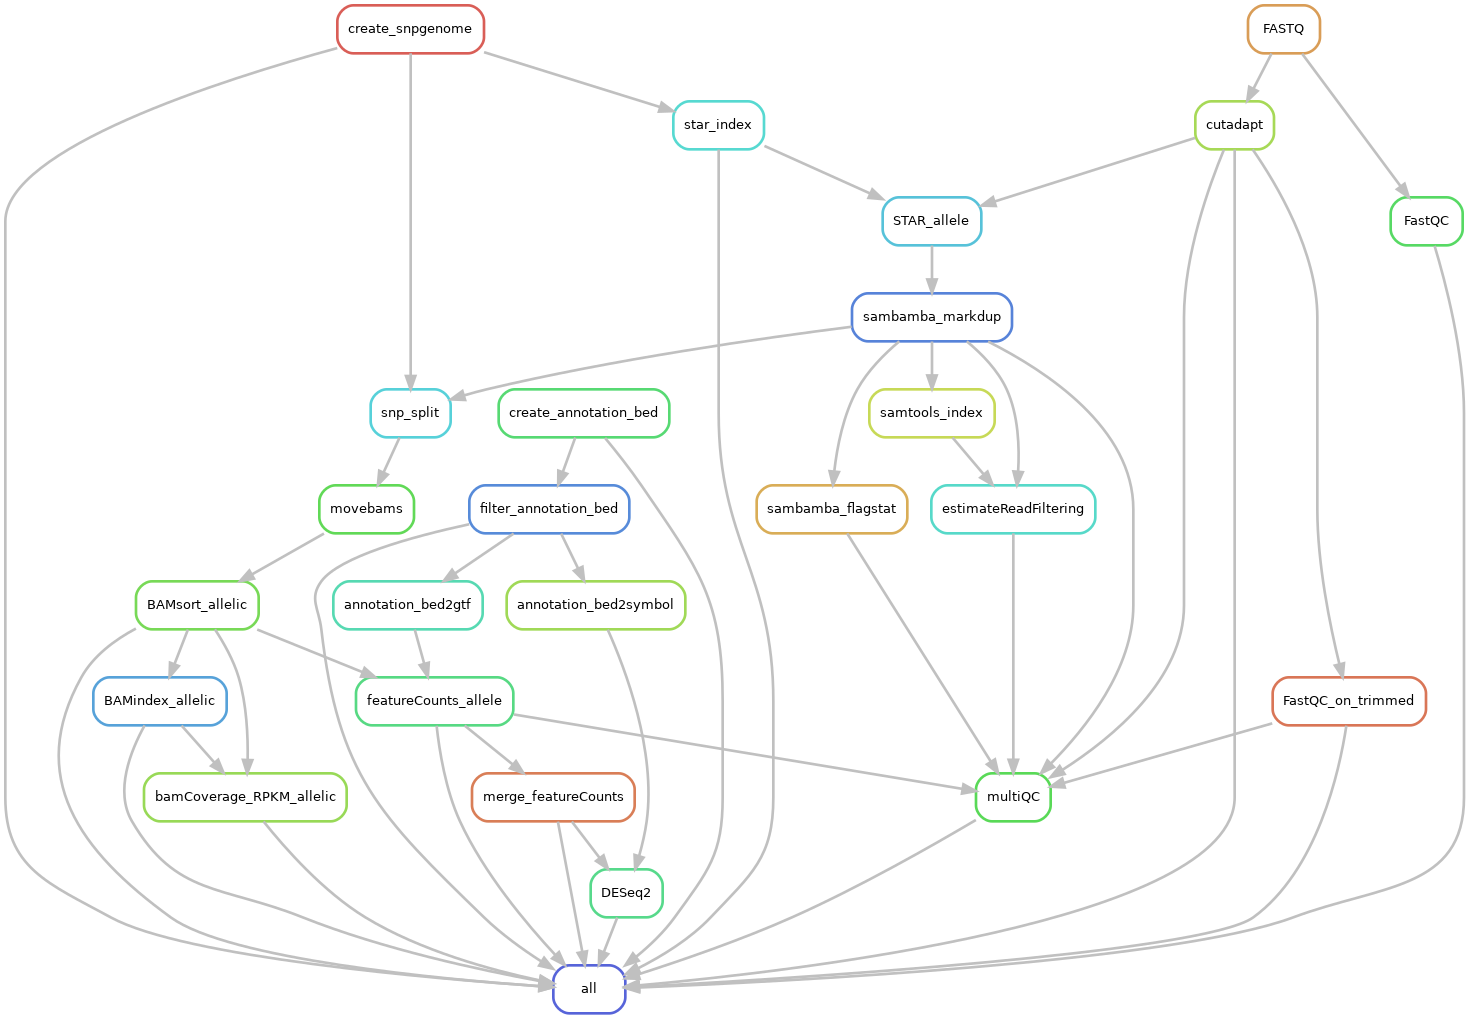
\includegraphics[width=0.95\linewidth,height=0.5\textheight]{figures/results_fig8} 

}

\caption[A directed acyclic graph (DAG) of the allele-specific RNA-seq analysis workflow]{\emph{\textbf{A directed acyclic graph (DAG) of the
allele-specific RNA-seq analysis workflow.} }The workflow begins with
creation of dual-hybrid genomes for user-defined strains of interest,
and ends with allele-specific differential expression analysis using a
statistical interaction based design. Optional quality-checks can be
performed via deepTools \textsuperscript{120} (not displayed here for
clarity). This workflow has been implemented in snakePipes.*}\label{fig:unnamed-chunk-13}
\end{figure}








\section{Conclusion and Outlook}\label{conclusion-and-outlook}

Various elements in eukaryotic genome, such as DNA sequences, chromatin
and the 3D topological structure act together to facilitate gene
regulation. Therefore, Integrative transcriptomic and epigenomic
analysis is becoming an important tool in understanding genomic
regulation. In this project, I performed the analysis of various
transcriptomic and epigenomic assays in order to understand the function
of members of the MSL complex, from flies to humans. To facilitate this,
we developed bioinformatic tools and workflows for the analysis of
transcription, histone marks and 3D conformation of the genome.
Application of our methods revealed a catalogue of high-resolution
boundaries in flies and their effect on transcription, the role of MSL
complex member MLE and H4K16ac in promoter usage in male flies, the
newly evolved function of MLE ortholog DHX9 in mammals, and finally an
interesting new insight into the role of the mammalian MSL complex on
the X-chromosome.

Future directions in studying MSLs would benefit from further
integration of data. For example, since most TAD boundaries in flies are
associated with promoters, an integration of 3D conformation and
promoter-profiling data could reveal the mechanism of how gene-by-gene
dosage compensation could be established at early embryogenesis via the
spreading of MSL-complex on X. Further, it It would be interesting to
explore the role of chromosome conformation in other scenarios, such as
the recently observed targeting of MSL2 on autosomes
\textsuperscript{183}. Unlike well studied functions of the MSLs in
\emph{Drosophila}, we have only recently started to understand the role
of MSLs in mammals, and in particular, its difference with the role of
another MOF associated complex, the NSLs. Rigorously designed ChIP-seq
experiments in presence of MSL and NSL knockout controls would be
required to avoid antibody non-specificity as well as to study the
dependence of MSL targeting on the NSL complex. Our understanding of the
role of H4K16ac in mammals would also be improved by studying its
relationship with other histone marks. Performing a full histone
profiling upon MSL and NSL depletion would be relatively simpler now due
to the development of highly multiplexed protocols
\textsuperscript{110}, enabling future studies to address such
questions. Further, development of technologies performing low-cell or
single cell epigenomics has provided new scope to study MSL biology in
tissues during development and differentiation. Methods for analysis of
such assays are yet in their infancy, and therefore would present
interesting challenges to work on in the near future.

\appendix

\chapter{Publications and
Manuscripts}\label{publications-and-manuscripts}

\section{Analysis of chromosome conformation in
flies}\label{analysis-of-chromosome-conformation-in-flies}
\begin{longtable}[]{@{}l@{}}
\toprule
\begin{minipage}[t]{0.97\columnwidth}\raggedright\strut
\textbf{High-resolution TADs reveal DNA sequences underlying genome
organization in flies.} Ramírez, F.*, \textbf{Bhardwaj, V.*}, Arrigoni,
L., Lam, K. C., Grüning, B. A., Villaveces, J., \ldots{} Manke, T.
\textbf{Nature communications (2018)}.
\url{doi:10.1038/s41467-017-02525-w} * shared authorship\strut
\end{minipage}\tabularnewline
\bottomrule
\end{longtable}
I contributed to the development of HiCExplorer and HiCBrowser (led by
Fidel Ramirez), and developed the Chorogenome Navigator resource. I
performed the analysis of motif combinations and boundary strength,
prediction of motifs, and relationship of TAD boundaries and
transcription (Fig 2, S2, 4, S4, 5 and S5). Together with Fidel Ramirez
and Thomas Manke I devised, wrote, and revised the manuscript.

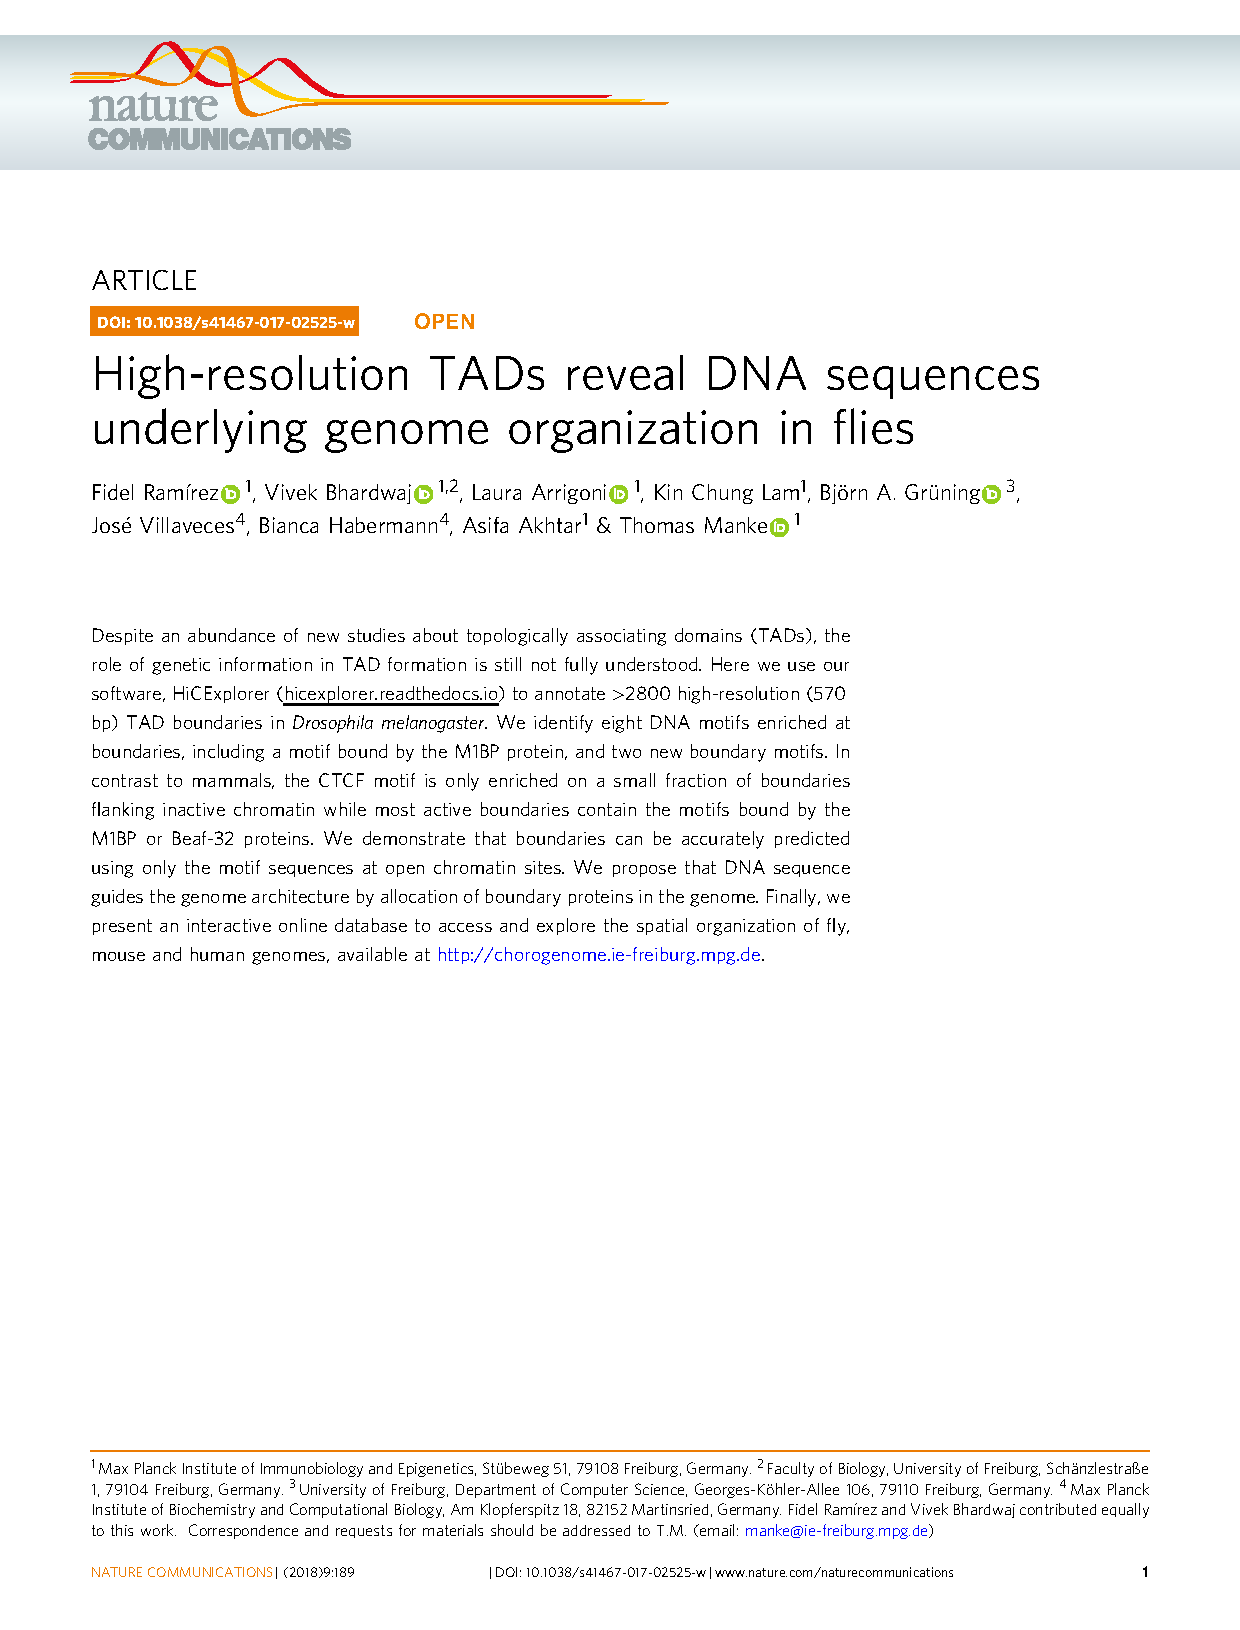
\includepdf[scale=0.9,pages=-,pagecommand={}, offset=0.3cm 0cm]{manuscripts/NatComm_2018_article.pdf}

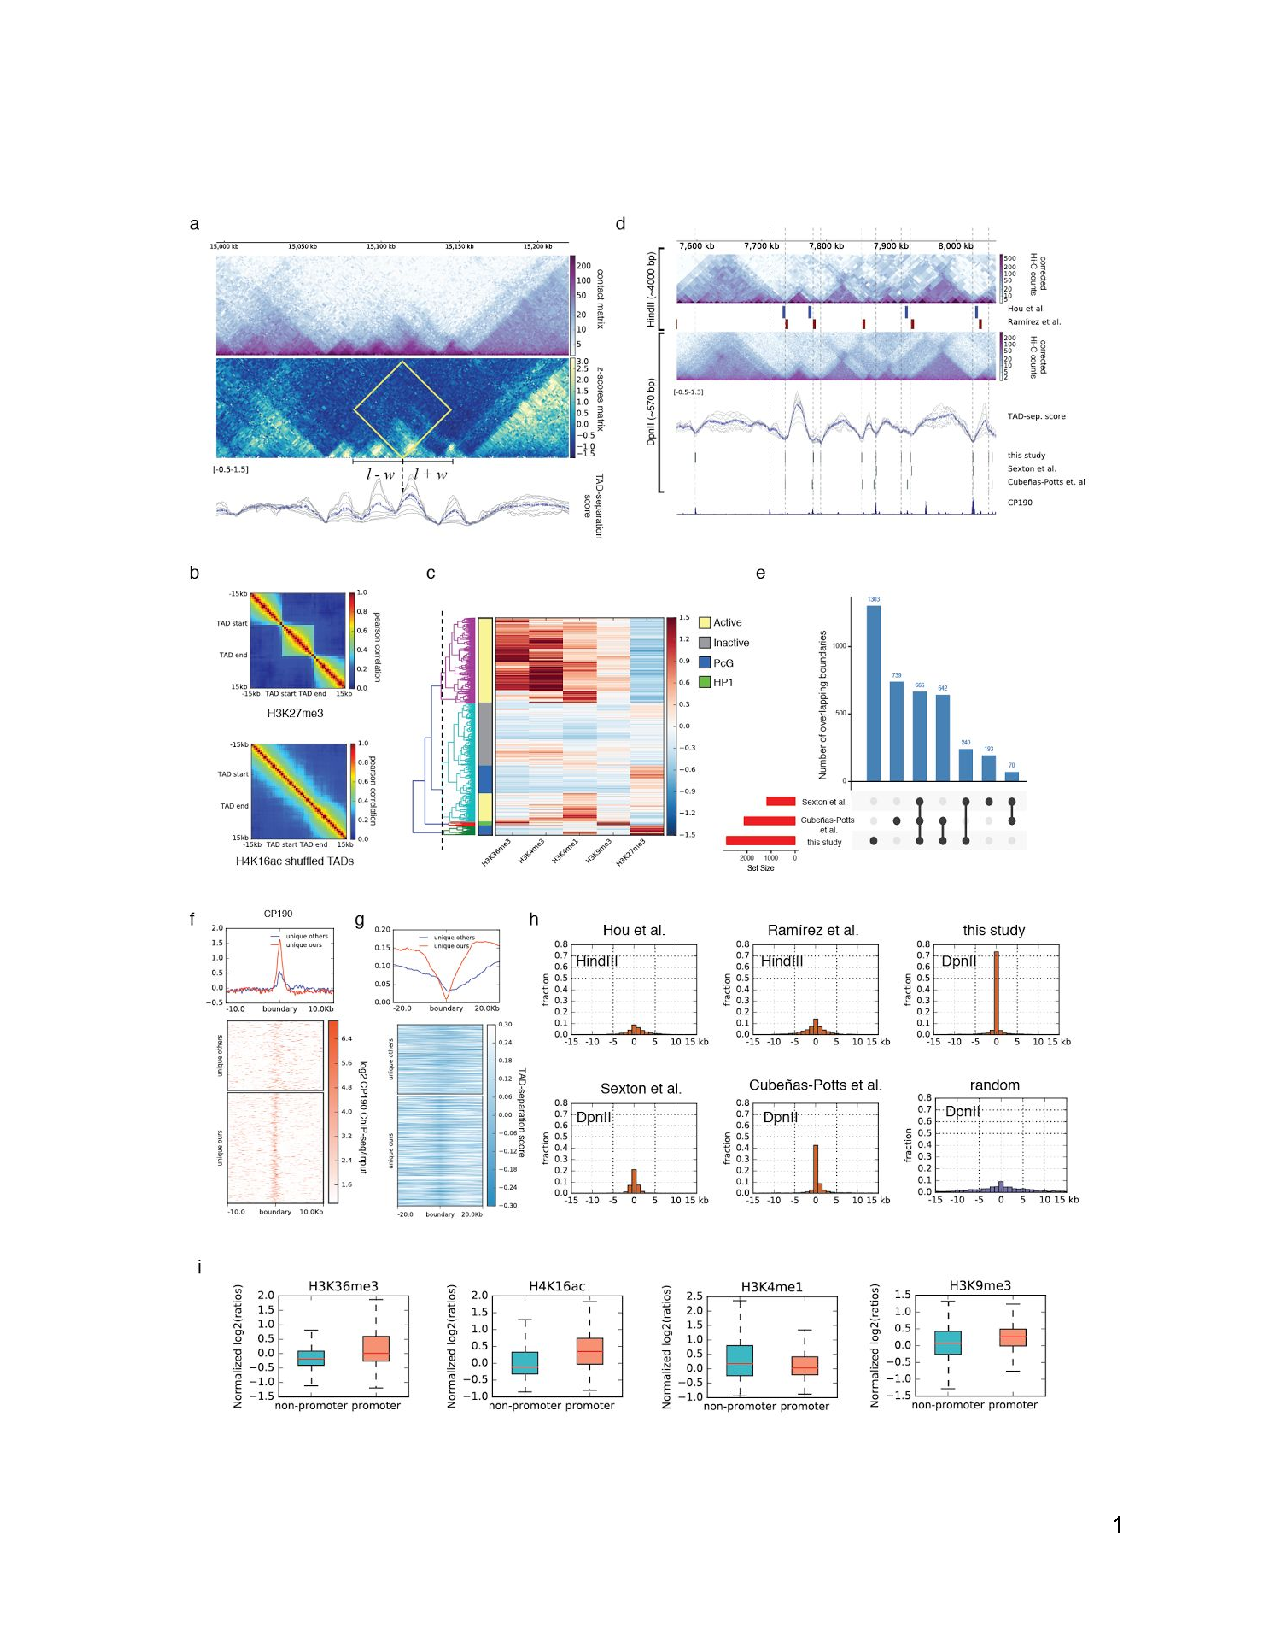
\includepdf[scale=0.9,pages=-,pagecommand={}, offset=0.3cm 0cm]{manuscripts/NatComm_2018_supple.pdf}

\section{Galaxy HiCExplorer}\label{galaxy-hicexplorer}
\begin{longtable}[]{@{}l@{}}
\toprule
\begin{minipage}[t]{0.97\columnwidth}\raggedright\strut
\textbf{Galaxy HiCExplorer: a web server for reproducible HiC data
analysis, quality control and visualization.} Wolff, J.,
\textbf{Bhardwaj, V.}, Nothjunge, S., Richard, G., Renschler, G.,
Gilsbach, R., \ldots{} Grüning, B.A. \textbf{Nucleic acids research
(2018).} \url{doi:10.1093/nar/gky504}\strut
\end{minipage}\tabularnewline
\bottomrule
\end{longtable}
I contributed to the development of HiCExplorer and designed the
template for the workflow used in the galaxy web server. I contributed
to the writing and revision of the manuscript along with Joachim Wolff
and other authors.

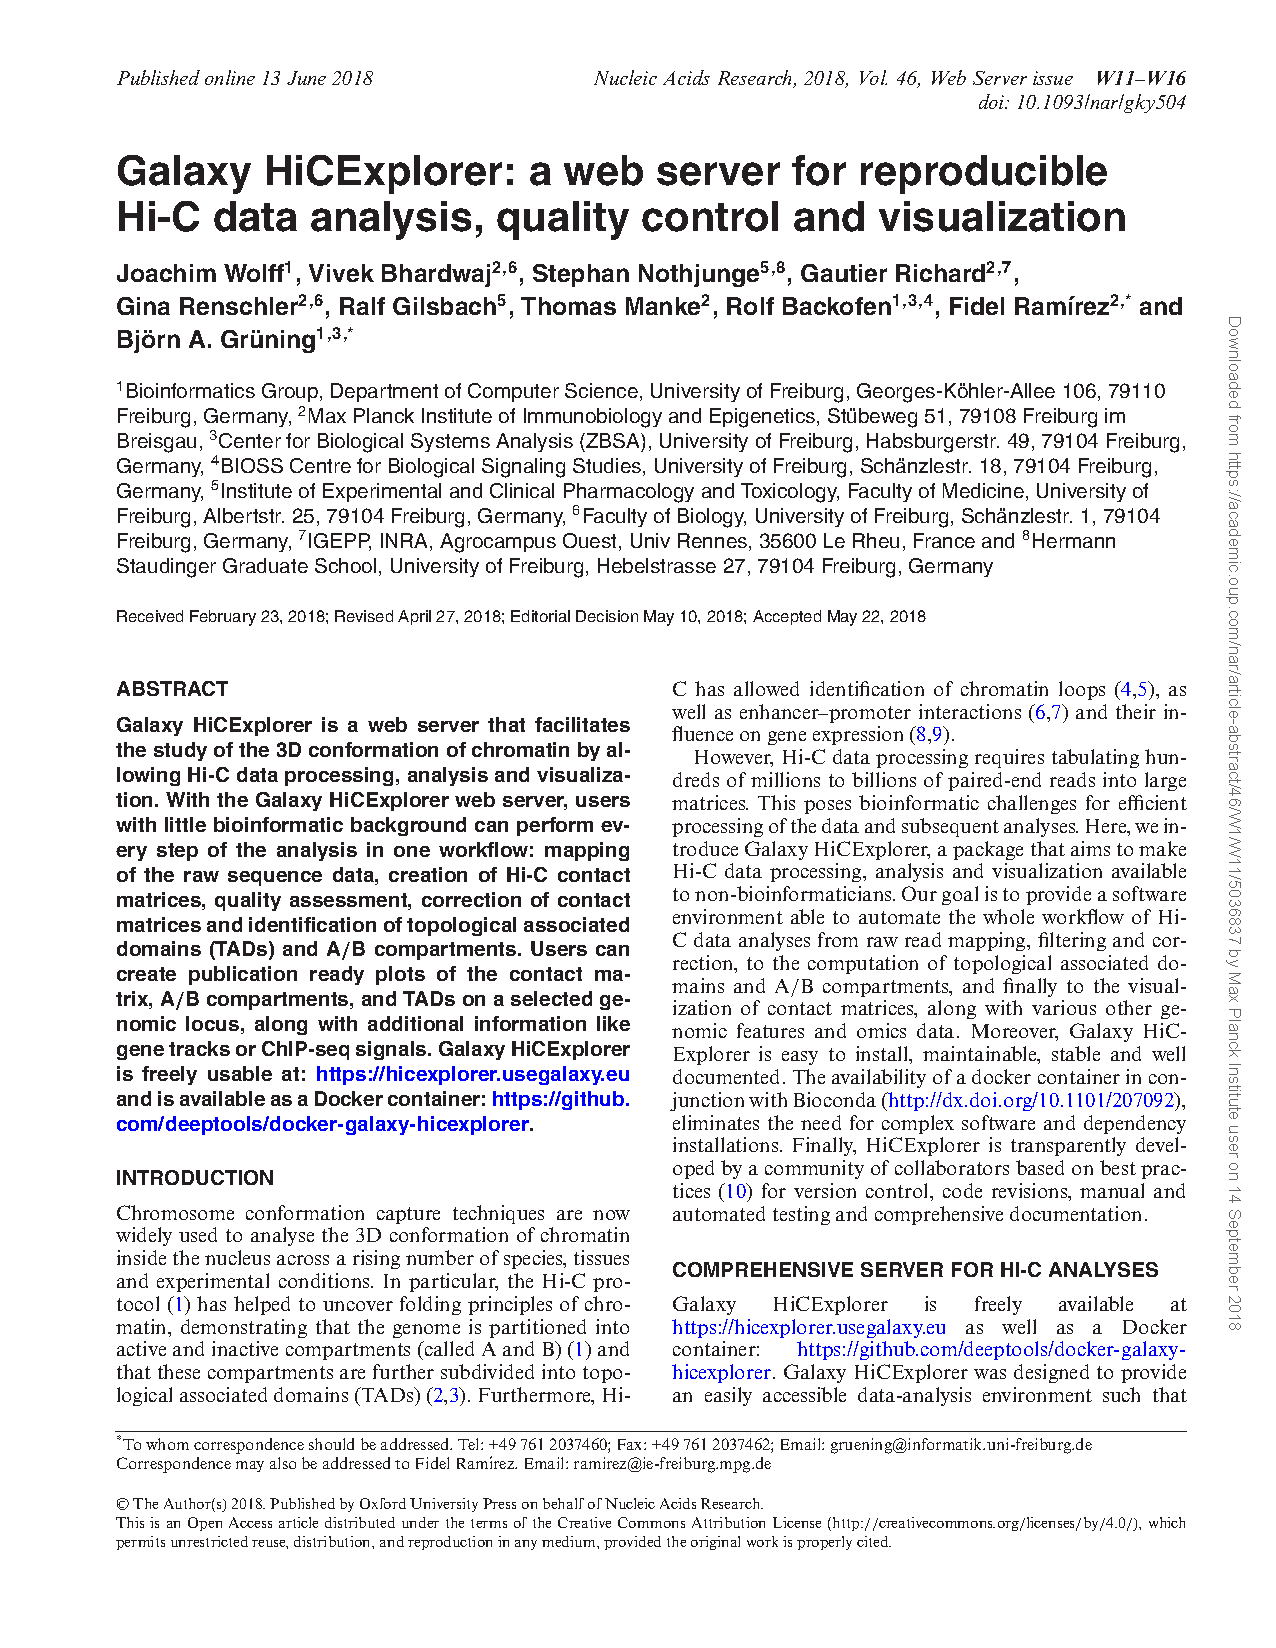
\includepdf[scale=0.9,pages=-,pagecommand={}, offset=0.3cm 0cm]{manuscripts/NAR_2018_article.pdf}

\section{Analysis of dosage compensation in flies via
promoter-profiling}\label{analysis-of-dosage-compensation-in-flies-via-promoter-profiling}
\begin{longtable}[]{@{}l@{}}
\toprule
\begin{minipage}[t]{0.97\columnwidth}\raggedright\strut
\textbf{Quantitative analysis of dosage compensation in flies using
promoter profiling} Bhardwaj V.*, Semplicio G*, Manke T, Akhtar A
\emph{(unpublished)}. * shared authorship\strut
\end{minipage}\tabularnewline
\bottomrule
\end{longtable}
I contributed to the development of the MAPCap protocol by providing the
analysis input, where all the experiments were performed by Giuseppe
Semplicio. I developed the icetea bioconductor package, performed all
the analysis presented in the paper, made the figures and wrote the
manuscript with input from Giuseppe Semplicio.

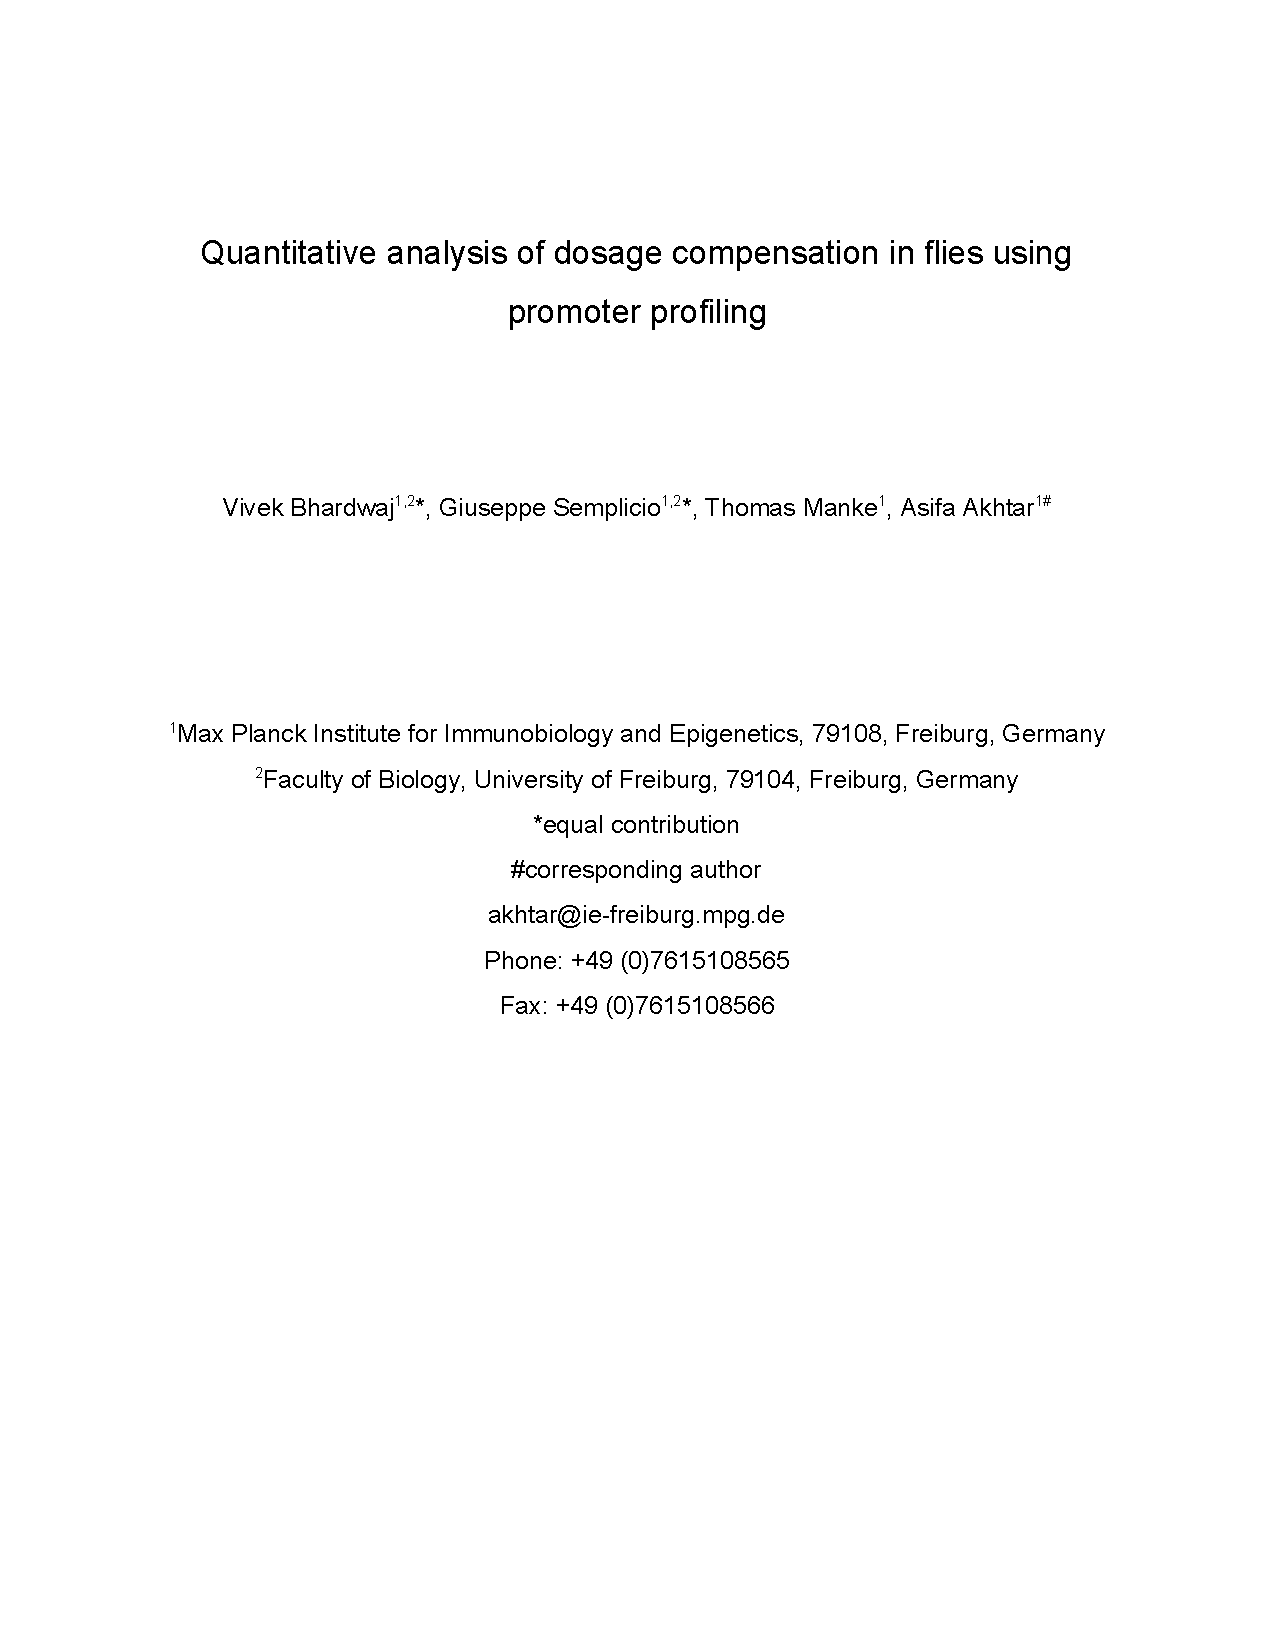
\includepdf[scale=0.9,pages=-,pagecommand={}, offset=0.3cm 0cm]{manuscripts/mapcap_paper_14-09-2018.pdf}

\section{Interaction of MLE ortholog DHX9 with Alu elements in the human
genome}\label{interaction-of-mle-ortholog-dhx9-with-alu-elements-in-the-human-genome}
\begin{longtable}[]{@{}l@{}}
\toprule
\begin{minipage}[t]{0.97\columnwidth}\raggedright\strut
\textbf{DHX9 suppresses RNA processing defects originating from the Alu
invasion of the human genome.} Aktaş, T., Avşar Ilık, İ., Maticzka, D.,
\textbf{Bhardwaj, V.}, Pessoa Rodrigues, C., Mittler, G., \ldots{}
Akhtar, A. \textbf{Nature (2017)}. \url{doi:10.1038/nature21715}\strut
\end{minipage}\tabularnewline
\bottomrule
\end{longtable}
I performed the analysis of UV-CLAP data for estimation of Alu
enrichment (Extended data Fig. 2 and 3) and performed the RNA-seq
analysis for detection of differential expression, splicing, circular
RNAs and RNA editing (Fig. 2a, 2b, 3a, Extended Data Figure 6, 7, 10). I
contributed to the writing and revision of the manuscript along with
Tugce Aktas, Ibrahim Ilik, Asifa Akhtar and other authors.

\includepdf[scale=0.9,pages=-,pagecommand={}, offset=0.3cm 0cm]{manuscripts/Nature_2017_article_supple.pdf}

\section{Update of the deepTools toolkit for exploring deep-sequencing
data}\label{update-of-the-deeptools-toolkit-for-exploring-deep-sequencing-data}
\begin{longtable}[]{@{}l@{}}
\toprule
\begin{minipage}[t]{0.97\columnwidth}\raggedright\strut
\textbf{deepTools2: a next generation web server for deep-sequencing
data analysis.} Ramírez, F., Ryan, D. P., Grüning, B., \textbf{Bhardwaj,
V.}, Kilpert, F., Richter, A. S., \ldots{} Manke, T. \textbf{Nucleic
acids research (2016)}. \url{doi:10.1093/nar/gkw257}\strut
\end{minipage}\tabularnewline
\bottomrule
\end{longtable}
I contributed to the development of deepTools2 (led by Fidel Ramirez and
Devon Ryan) through features and bugfixes, and to the testing and update
of its documentation and the galaxy server. I helped with the writing
and revision of the manuscript by Fidel Ramirez and other authors.

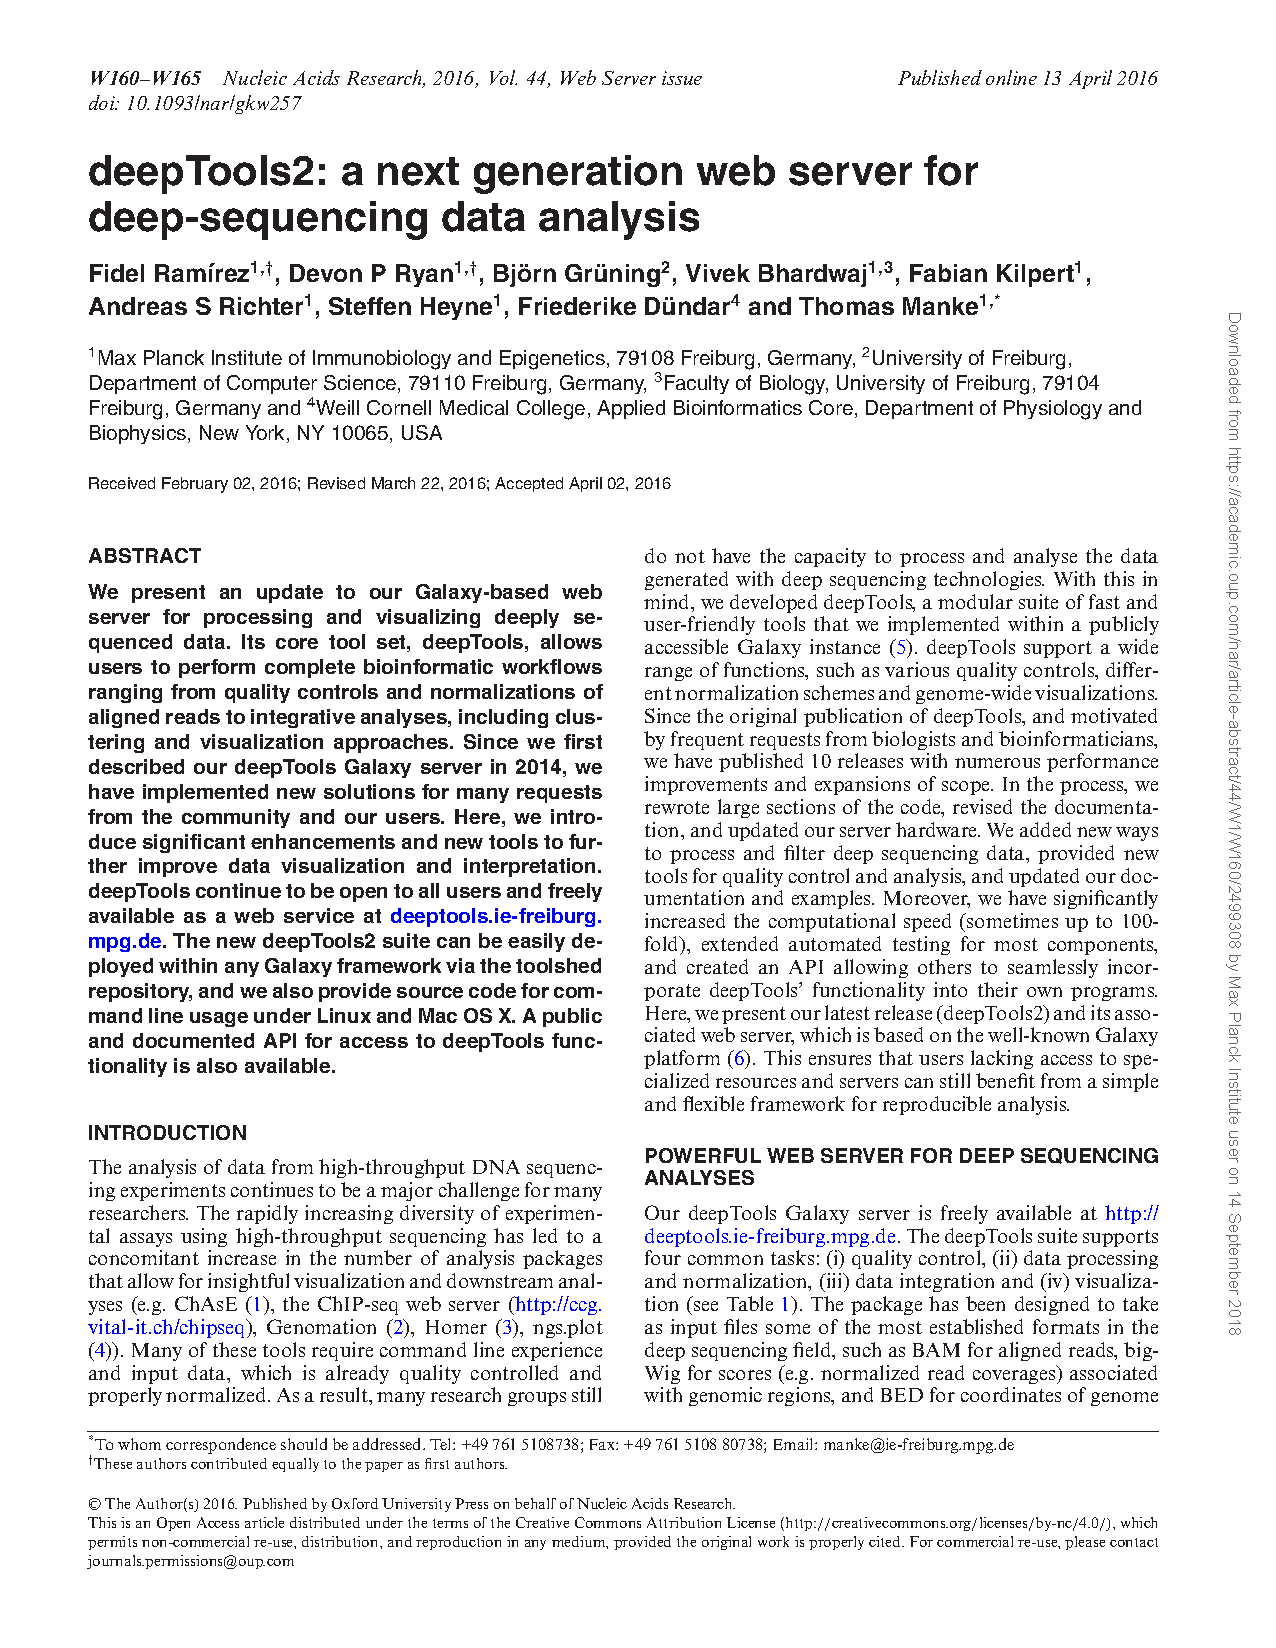
\includepdf[scale=0.9,pages=-,pagecommand={}, offset=0.3cm 0cm]{manuscripts/NAR_2016_article.pdf}

\section{snakePipes enables reproducible epigenomic
analysis}\label{snakepipes-enables-reproducible-epigenomic-analysis}
\begin{longtable}[]{@{}l@{}}
\toprule
\begin{minipage}[t]{0.97\columnwidth}\raggedright\strut
\textbf{snakePipes enable flexible, scalable and integrative epigenomic
analysis.} \textbf{Bhardwaj, V.*}, Heyne, S.*, Sikora, K., Rabbani, L.,
Rauer, M., Kilpert, F., \ldots{} Manke, T. \textbf{bioRxiv (2018).}
\url{doi:10.1101/407312} * shared authorship\strut
\end{minipage}\tabularnewline
\bottomrule
\end{longtable}
I developed the allele-specific and HiC workflows and contributed to
DNA-mapping, ChIP-seq, ATAC-seq and RNA-seq workflows and documentation.
I performed the analysis, prepared the figures and wrote the manuscript
with input from all authors.

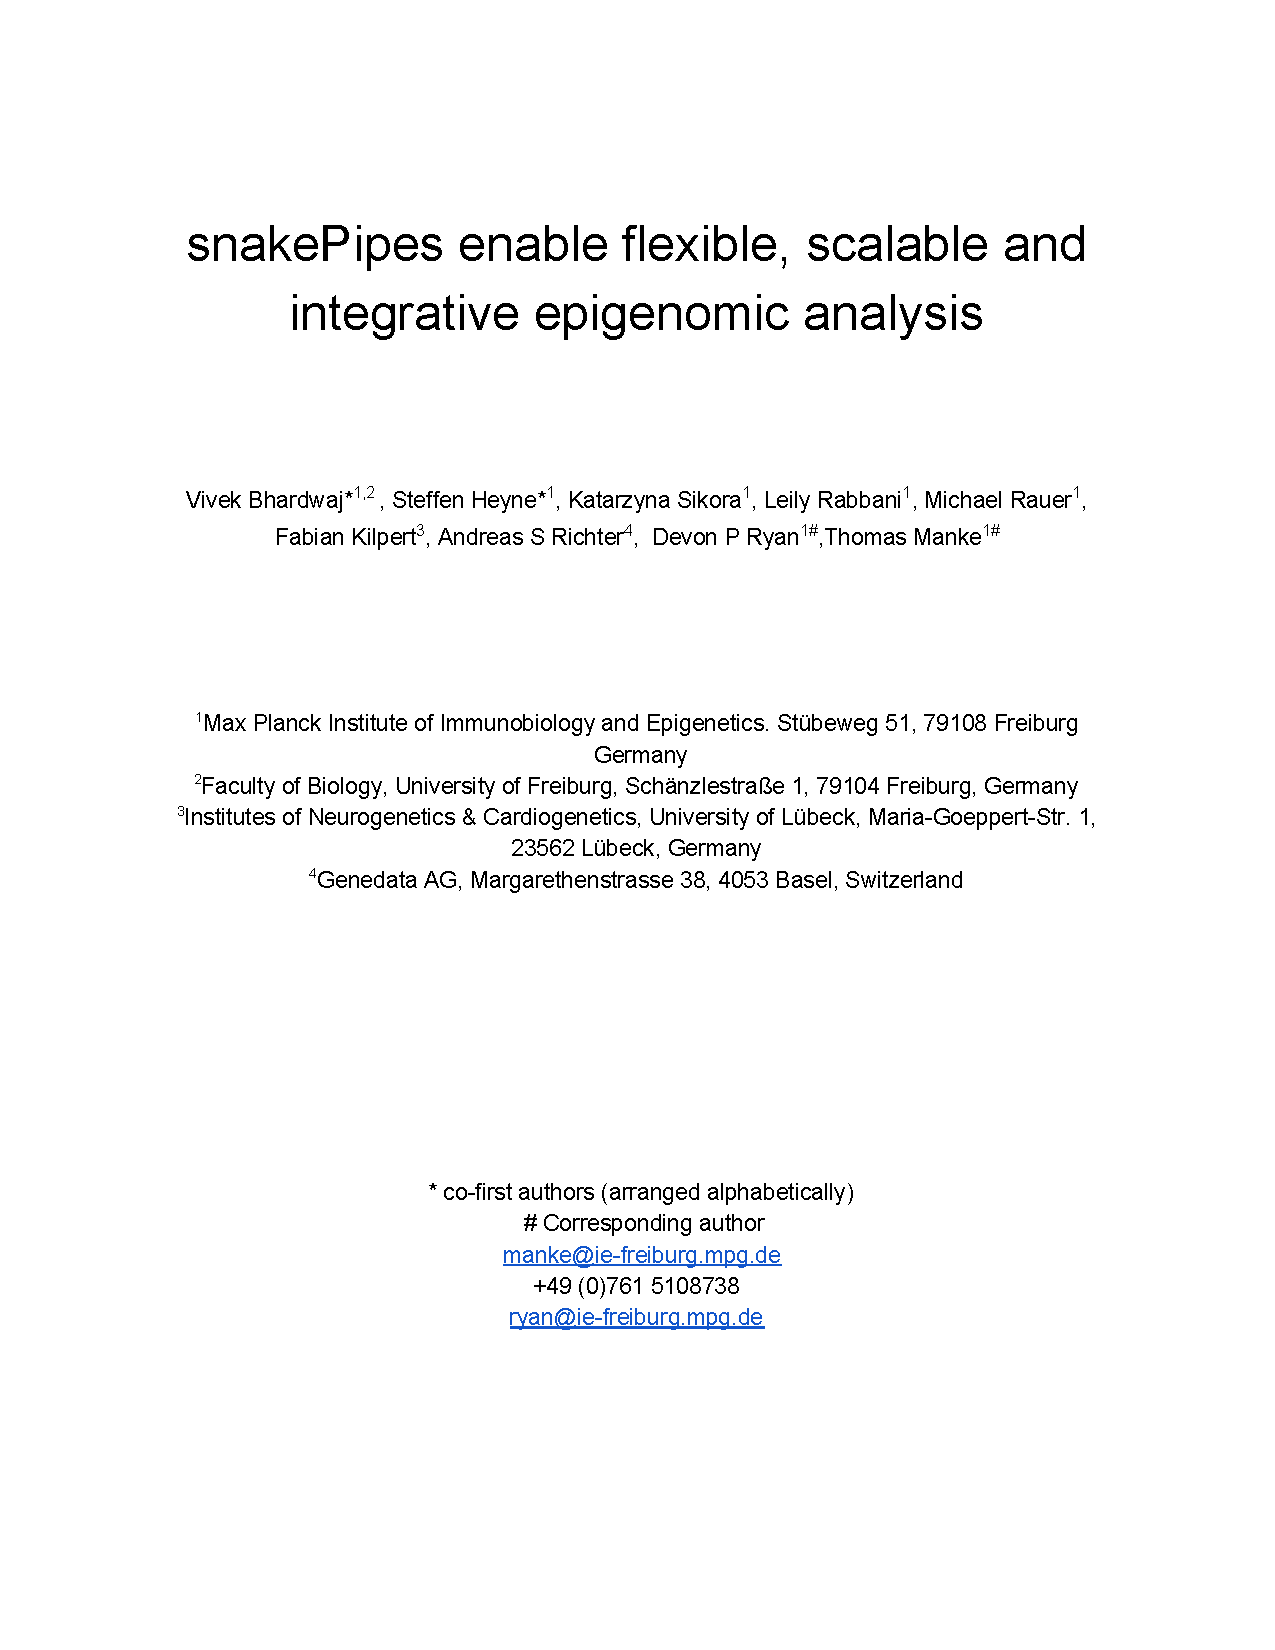
\includepdf[scale=0.9,pages=-,pagecommand={}, offset=0.3cm 0cm]{manuscripts/snakepipes_manuscript_10-09-2018.pdf}

\chapter{Supplemental information}\label{supplemental-information}

\clearpage

\section{Definitions}\label{definitions}

\textbf{DNA :} Deoxyribonucleic acid. It is a negatively charged, large
polymer composed of a combination of four bases (Adenine, Guanine,
Cytosine, Thymine) and stores genetic information in living organisms.

\textbf{Histones :} Negatively charged proteins that wrap the DNA in the
nucleus. Apart from providing structural support, the histones are also
critical in gene regulation.

\textbf{Chromatin :} In order to efficiently pack inside the nucleus,
DNA is wrapped around positively charged proteins called ``histones'' in
order to form ``chromatin''.

\textbf{Transcription :} production of messenger RNA or ``mRNA'' through
DNA, by the protein ``RNA polymerase''

\textbf{Translation :} production of proteins through mRNA by
RNA-protein complex ``Ribosome''

\textbf{Histone Code :} Numerous post-translational modifications are
possible on histone marks, usually referred to as histone code
\textsuperscript{19}.

\textbf{Readers} : Proteins that recognize histone marks
\textsuperscript{206}. Readers either perform various biochemical
activities in response to the histone code, or interact with other
proteins that perform these activities eventually leading to the
regulation of target genes \textsuperscript{207,208}.

\textbf{Writers :} The proteins that deposit histone marks either in
response to change in cellular environment, through genetic programming
(eg. during development), or in response to another histone mark
\textsuperscript{209}.

\textbf{Transcription factors (TFs) :} Classically, TFs are described as
having a DNA binding domain, and a trans-activation domain, which
activates RNAP-II machinery to facilitate transcription
\textsuperscript{210}. TFs could also recruit various co-activators or
co-repressors which add additional complexity to transcriptional
regulation \textsuperscript{211}.

\textbf{General TFs :} Usually, transcription factors associated with
core RNAP-II machinery are referred to as ``general transcription
factors'' (GTFs) {[}\^{}212\^{}{]} while the specific transcription
factors associated with enhancers and RNAP-II under specific conditions,
are referred simply as ``transcription factors'' (TFs)
\textsuperscript{213}.

\textbf{DNA motifs :} Short DNA sequences that are recognized by DNA
binding domains of various regulatory proteins.

\textbf{4-cutters :} Restriction enzymes with 4 base-pair recognition
sites on DNA. Eg. Dpn-II

\textbf{6-cutters :} Restriction enzymes with 6 base-pair recognition
sites on DNA. Eg. Hind-III

\section{Tables}\label{tables}

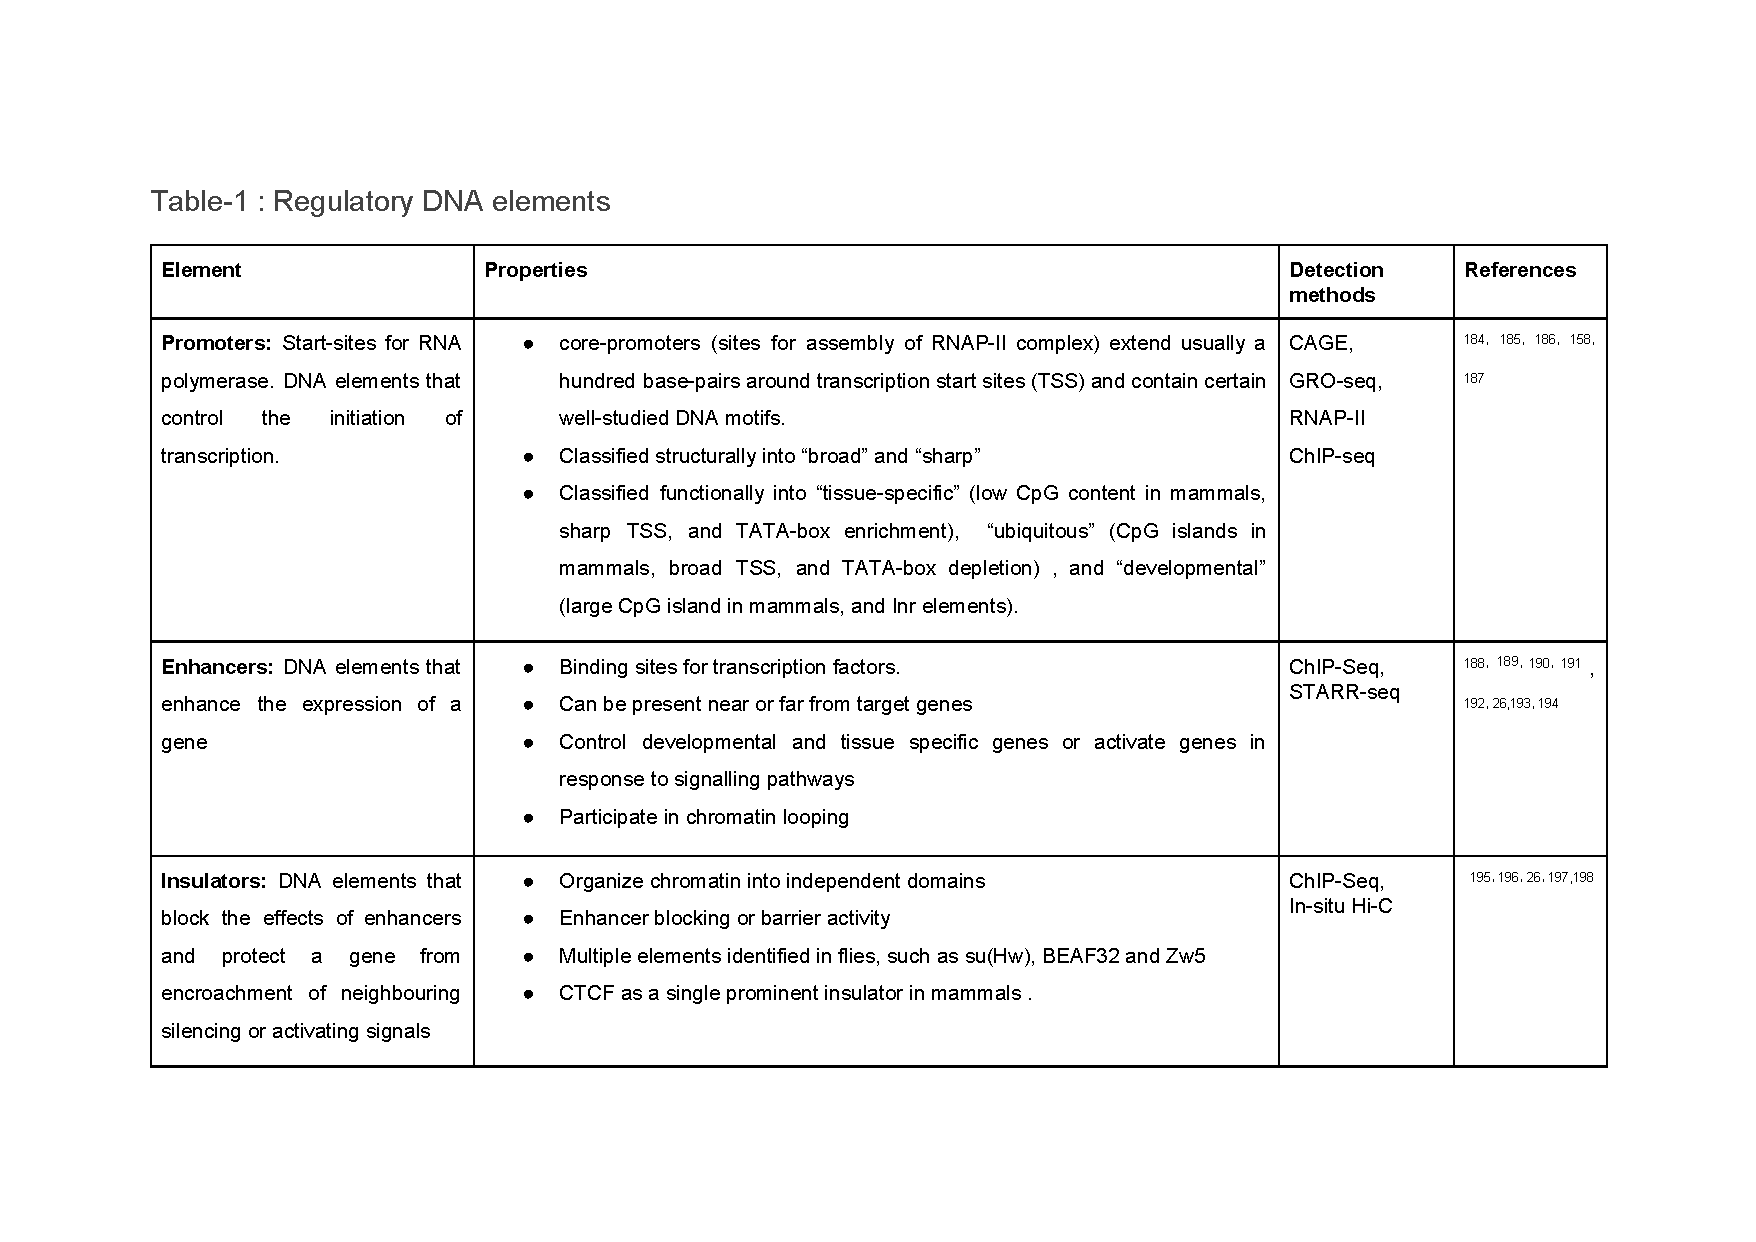
\includepdf[scale=0.9,pages=-,pagecommand={}, offset=0.3cm 0cm,angle=90]{data/Table-1.pdf}

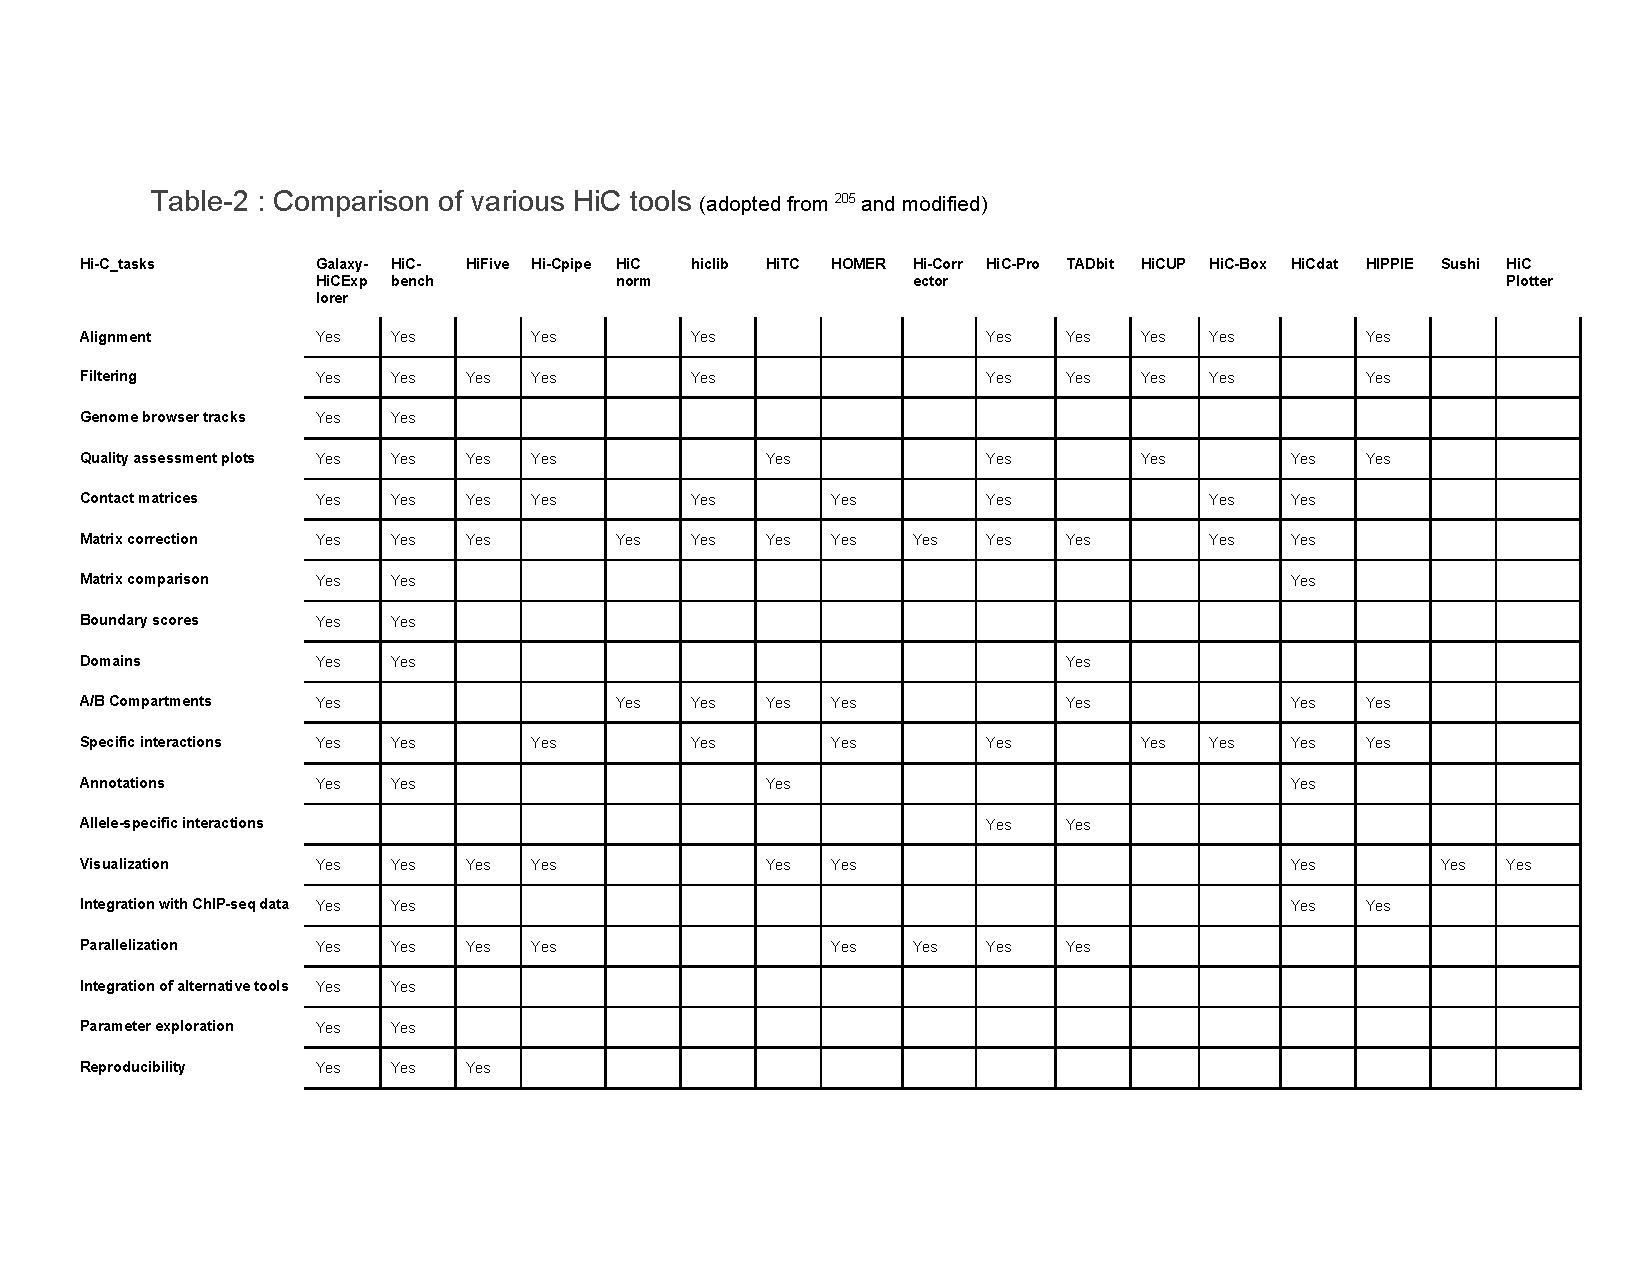
\includepdf[scale=0.9,pages=-,pagecommand={}, offset=0.3cm 0cm,angle=90]{data/Table-2.pdf}

\chapter{Academic Vita}\label{academic-vita}

\setstretch{1.2}

\subsubsection{EDUCATION}\label{education}

\textbf{Since October 2014 : PhD Candidate}

Max Planck Institute of Immunobiology and Epigenetics and Faculty of
Biology, University of Freiburg

\textbf{2011 - 2013 : Master of Science (Biomedical Sciences)}

University of Delhi, New Delhi, India

Thesis : Exploring the novel regulatory mechanisms of gene regulation by
Human Alu elements.

\textbf{2008 - 2011 : Bachelor of Science (Biomedical Sciences)}

University of Delhi, New Delhi, India

Thesis: Gene Ontology Annotation of Mycobacterium tuberculosis H37Rv
genes.

\textbf{2008 : High School Diploma}

Central Board of Secondary Education, India

\subsubsection{PUBLICATIONS/PREPRINTS}\label{publicationspreprints}

\textbf{snakePipes enable flexible, scalable and integrative epigenomic
analysis.} \textbf{Bhardwaj, V.*}, Heyne, S.*, Sikora, K., Rabbani, L.,
Rauer, M., Kilpert, F., \ldots{} Manke, T. \textbf{bioRxiv (2018).}
\href{https://doi.org/10.1101/407312}{{https://doi.org/10.1101/407312}}

\textbf{High-resolution TADs reveal DNA sequences underlying genome
organization in flies.} Ramírez, F.*, \textbf{Bhardwaj, V.*}, Arrigoni,
L., Lam, K. C., Grüning, B. A., Villaveces, J., \ldots{} Manke, T.
\textbf{Nature communications (2018)}.
\href{https://www.nature.com/articles/s41467-017-02525-w}{{doi:10.1038/s41467-017-02525-w}}

\textbf{Galaxy HiCExplorer: a web server for reproducible Hi-C data
analysis, quality control and visualization.} Wolff, J.,
\textbf{Bhardwaj, V.}, Nothjunge, S., Richard, G., Renschler, G.,
Gilsbach, R., \ldots{} Grüning, B. A. \textbf{Nucleic acids research
(2018).}
\href{http://doi.org/10.1093/nar/gky504}{{doi.org/10.1093/nar/gky504}}

\textbf{Community-Driven Data Analysis Training for Biology.} Batut, B.,
Hiltemann, S., Bagnacani, A., Baker, D., \textbf{Bhardwaj, V.}, Blank,
C., \ldots{} Grüning, B. \textbf{Cell Systems* (2018).}
\href{https://doi.org/10.1016/j.cels.2018.05.012}{{doi:10.1016/j.cels.2018.05.012}}

\textbf{DHX9 suppresses RNA processing defects originating from the Alu
invasion of the human genome.} Aktaş, T., Avşar Ilık, İ., Maticzka, D.,
\textbf{Bhardwaj, V.}, Pessoa Rodrigues, C., Mittler, G., \ldots{}
Akhtar, A. \textbf{Nature (2017)}.
\href{https://www.nature.com/articles/nature21715}{{doi:10.1038/nature21715}}

\textbf{deepTools2: a next generation web server for deep-sequencing
data analysis.} Ramírez, F., Ryan, D. P., Grüning, B., \textbf{Bhardwaj,
V.}, Kilpert, F., Richter, A. S., \ldots{} Manke, T. \textbf{Nucleic
acids research (2016)}.
\href{http://dx.doi.org/10.1093/nar/gku365}{{doi:10.1093/nar/gkw257}}

\textbf{MOF maintains transcriptional programs regulating cellular
stress response.} Sheikh, B. N., Bechtel-Walz, W., Lucci, J., Karpiuk,
O., Hild, I., Hartleben, B., \textbf{**}\ldots{} Akhtar, A.
\textbf{Oncogene* (2016)}.
\href{https://doi.org/10.1038/onc.2015.335}{{doi:10.1038/onc.2015.335}}

\textbf{Alu-miRNA interactions modulate transcript isoform diversity in
stress response and reveal signatures of positive selection.} Pandey,
R., Bhattacharya, A., \textbf{Bhardwaj, V.}, Jha, V., Mandal, A. K., \&
Mukerji, M. \textbf{Scientific Reports* (2016)}.
\href{http://dx.doi.org/10.1038/srep32348}{{doi:10.1038/srep32348}}

\textbf{Draft Genome Sequence of Urease-Producing Sporosarcina pasteurii
with Potential Application in Biocement Production.} Tiwari, P. K.*,
Joshi, K.*, Rehman, R.*, \textbf{Bhardwaj, V.*}, Shamsudheen, K. V.,
Sivasubbu, S., \& Scaria, V. \textbf{Genome Announcements* (2014)}.
\href{https://doi.org/10.1128/genomeA.01256-13}{{doi:10.1128/genomeA.01256-13}}

\textbf{The Zebrafish GenomeWiki: a crowdsourcing approach to connect
the long tail for zebrafish gene annotation.} Singh, M., Bhartiya, D.,
Maini, J., Sharma, M., Singh, A. R., Kadarkaraisamy, S.,
\textbf{***}\ldots{} Sivasubbu, S. \textbf{Database: The Journal of
Biological Databases and Curation* (2014)}
\href{https://doi.org/10.1093/database/bau011}{{doi:10.1093/database/bau011}}

* contributed equally

** author at 10th position

*** author at 27th position

\backmatter

\chapter*{References}\label{references}
\addcontentsline{toc}{chapter}{References}

\noindent

1. Crick, F. Central dogma of molecular biology. \emph{Nature}
\textbf{227,} 561--563 (1970).

2. Epp, C. D. Definition of a gene. \emph{Nature} \textbf{389,} 537
(1997).

3. Gerstein, M. B. \emph{et al.} What is a gene, post-ENCODE? History
and updated definition. \emph{Genome Res.} \textbf{17,} 669--681 (2007).

4. Berthelot, C., Villar, D., Horvath, J. E., Odom, D. T. \& Flicek, P.
Complexity and conservation of regulatory landscapes underlie
evolutionary resilience of mammalian gene expression. \emph{Nat Ecol
Evol} \textbf{2,} 152--163 (2018).

5. Villegas, V. E. \& Zaphiropoulos, P. G. Neighboring gene regulation
by antisense long non-coding RNAs. \emph{Int. J. Mol. Sci.} \textbf{16,}
3251--3266 (2015).

6. Catalanotto, C., Cogoni, C. \& Zardo, G. MicroRNA in Control of Gene
Expression: An Overview of Nuclear Functions. \emph{Int. J. Mol. Sci.}
\textbf{17,} (2016).

7. Engreitz, J. M., Ollikainen, N. \& Guttman, M. Long non-coding RNAs:
spatial amplifiers that control nuclear structure and gene expression.
\emph{Nat. Rev.~Mol. Cell Biol.} \textbf{17,} 756--770 (2016).

8. Siomi, H. \& Dreyfuss, G. RNA-binding proteins as regulators of gene
expression. \emph{Curr. Opin. Genet. Dev.} \textbf{7,} 345--353 (1997).

9. Berger, S. L., Kouzarides, T., Shiekhattar, R. \& Shilatifard, A. An
operational definition of epigenetics. \emph{Genes Dev.} \textbf{23,}
781--783 (2009).

10. Shendure, J. \emph{et al.} Accurate multiplex polony sequencing of
an evolved bacterial genome. \emph{Science} \textbf{309,} 1728--1732
(2005).

11. Schuster, S. C. Next-generation sequencing transforms today's
biology. \emph{Nat. Methods} \textbf{5,} 16--18 (2008).

12. Griffiths, P. E. In what sense does `nothing make sense except in
the light of evolution'? \emph{Acta Biotheor.} \textbf{57,} 11--32
(2009).

13. Mouse Genome Sequencing Consortium \emph{et al.} Initial sequencing
and comparative analysis of the mouse genome. \emph{Nature}
\textbf{420,} 520--562 (2002).

14. Church, D. M. \emph{et al.} Lineage-specific biology revealed by a
finished genome assembly of the mouse. \emph{PLoS Biol.} \textbf{7,}
e1000112 (2009).

15. Rands, C. M., Meader, S., Ponting, C. P. \& Lunter, G. 8.2\% of the
Human genome is constrained: variation in rates of turnover across
functional element classes in the human lineage. \emph{PLoS Genet.}
\textbf{10,} e1004525 (2014).

16. Graur, D. An Upper Limit on the Functional Fraction of the Human
Genome. \emph{Genome Biol. Evol.} \textbf{9,} 1880--1885 (2017).

17. ENCODE Project Consortium. An integrated encyclopedia of DNA
elements in the human genome. \emph{Nature} \textbf{489,} 57--74 (2012).

18. Riethoven, J.-J. M. Regulatory Regions in DNA: Promoters, Enhancers,
Silencers, and Insulators. in \emph{Computational Biology of
Transcription Factor Binding} (ed. Ladunga, I.) 33--42 (Humana Press,
2010).

19. Huang, H., Sabari, B. R., Garcia, B. A., Allis, C. D. \& Zhao, Y.
SnapShot: histone modifications. \emph{Cell} \textbf{159,} 458--458.e1
(2014).

20. Fuhrmann, G. \emph{et al.} Mouse germline restriction of Oct4
expression by germ cell nuclear factor. \emph{Dev. Cell} \textbf{1,}
377--387 (2001).

21. Feldman, N. \emph{et al.} G9a-mediated irreversible epigenetic
inactivation of Oct-3/4 during early embryogenesis. \emph{Nat. Cell
Biol.} \textbf{8,} 188--194 (2006).

22. Smallwood, A. \& Ren, B. Genome organization and long-range
regulation of gene expression by enhancers. \emph{Curr. Opin. Cell
Biol.} \textbf{25,} 387--394 (2013).

23. Cullen, K. E., Kladde, M. P. \& Seyfred, M. A. Interaction between
transcription regulatory regions of prolactin chromatin. \emph{Science}
\textbf{261,} 203--206 (1993).

24. Lieberman-Aiden, E. \emph{et al.} Comprehensive mapping of
long-range interactions reveals folding principles of the human genome.
\emph{Science} \textbf{326,} 289--293 (2009).

25. Dixon, J. R. \emph{et al.} Topological domains in mammalian genomes
identified by analysis of chromatin interactions. \emph{Nature}
\textbf{485,} 376--380 (2012).

26. Rao, S. S. P. \emph{et al.} A 3D map of the human genome at kilobase
resolution reveals principles of chromatin looping. \emph{Cell}
\textbf{159,} 1665--1680 (2014).

27. Dixon, J. R., Gorkin, D. U. \& Ren, B. Chromatin Domains: The Unit
of Chromosome Organization. \emph{Mol. Cell} \textbf{62,} 668--680
(2016).

28. Phillips-Cremins, J. E. \& Corces, V. G. Chromatin insulators:
linking genome organization to cellular function. \emph{Mol. Cell}
\textbf{50,} 461--474 (2013).

29. de Laat, W. \& Duboule, D. Topology of mammalian developmental
enhancers and their regulatory landscapes. \emph{Nature} \textbf{502,}
499--506 (2013).

30. Vietri Rudan, M. \emph{et al.} Comparative Hi-C reveals that CTCF
underlies evolution of chromosomal domain architecture. \emph{Cell Rep.}
\textbf{10,} 1297--1309 (2015).

31. Phillips, J. E. \& Corces, V. G. CTCF: master weaver of the genome.
\emph{Cell} \textbf{137,} 1194--1211 (2009).

32. Nicodemi, M. \& Pombo, A. Models of chromosome structure.
\emph{Curr. Opin. Cell Biol.} \textbf{28,} 90--95 (2014).

33. Alipour, E. \& Marko, J. F. Self-organization of domain structures
by DNA-loop-extruding enzymes. \emph{Nucleic Acids Res.} \textbf{40,}
11202--11212 (2012).

34. Sanborn, A. L. \emph{et al.} Chromatin extrusion explains key
features of loop and domain formation in wild-type and engineered
genomes. \emph{Proc. Natl. Acad. Sci. U. S. A.} \textbf{112,} E6456--65
(2015).

35. Yardımcı, G. G. \& Noble, W. S. Predictive model of 3D domain
formation via CTCF-mediated extrusion. \emph{Proc. Natl. Acad. Sci. U.
S. A.} \textbf{112,} 14404--14405 (2015).

36. Fudenberg, G. \emph{et al.} Formation of Chromosomal Domains by Loop
Extrusion. \emph{Cell Rep.} \textbf{15,} 2038--2049 (2016).

37. Goloborodko, A., Marko, J. F. \& Mirny, L. A. Chromosome Compaction
by Active Loop Extrusion. \emph{Biophys. J.} \textbf{110,} 2162--2168
(2016).

38. Nuebler, J., Fudenberg, G., Imakaev, M., Abdennur, N. \& Mirny, L.
A. Chromatin organization by an interplay of loop extrusion and
compartmental segregation. \emph{Proc. Natl. Acad. Sci. U. S. A.}
\textbf{115,} E6697--E6706 (2018).

39. Nora, E. P. \emph{et al.} Targeted Degradation of CTCF Decouples
Local Insulation of Chromosome Domains from Genomic
Compartmentalization. \emph{Cell} \textbf{169,} 930--944.e22 (2017).

40. Rao, S. S. P. \emph{et al.} Cohesin Loss Eliminates All Loop
Domains. \emph{Cell} \textbf{171,} 305--320.e24 (2017).

41. Haarhuis, J. H. I. \emph{et al.} The Cohesin Release Factor WAPL
Restricts Chromatin Loop Extension. \emph{Cell} \textbf{169,}
693--707.e14 (2017).

42. Richterova, J., Huraiova, B. \& Gregan, J. Genome Organization:
Cohesin on the Move. \emph{Mol. Cell} \textbf{66,} 444--445 (2017).

43. Terakawa, T. \emph{et al.} The condensin complex is a
mechanochemical motor that translocates along DNA. \emph{Science}
\textbf{358,} 672--676 (2017).

44. Ganji, M. \emph{et al.} Real-time imaging of DNA loop extrusion by
condensin. \emph{Science} \textbf{360,} 102--105 (2018).

45. Stigler, J., Çamdere, G. Ö., Koshland, D. E. \& Greene, E. C.
Single-Molecule Imaging Reveals a Collapsed Conformational State for
DNA-Bound Cohesin. \emph{Cell Rep.} \textbf{15,} 988--998 (2016).

46. Ulianov, S. V. \emph{et al.} Active chromatin and transcription play
a key role in chromosome partitioning into topologically associating
domains. \emph{Genome Res.} \textbf{26,} 70--84 (2016).

47. Hug, C. B., Grimaldi, A. G., Kruse, K. \& Vaquerizas, J. M.
Chromatin Architecture Emerges during Zygotic Genome Activation
Independent of Transcription. \emph{Cell} \textbf{169,} 216--228.e19
(2017).

48. Heinz, S. \emph{et al.} Transcription Elongation Can Affect Genome
3D Structure. \emph{Cell} \textbf{174,} 1522--1536.e22 (2018).

49. Graves, J. A. M. Evolution of vertebrate sex chromosomes and dosage
compensation. \emph{Nat. Rev.~Genet.} \textbf{17,} 33--46 (2016).

50. Okamoto, I., Otte, A. P., Allis, C. D., Reinberg, D. \& Heard, E.
Epigenetic dynamics of imprinted X inactivation during early mouse
development. \emph{Science} \textbf{303,} 644--649 (2004).

51. Escamilla-Del-Arenal, M., da Rocha, S. T. \& Heard, E. Evolutionary
diversity and developmental regulation of X-chromosome inactivation.
\emph{Hum. Genet.} \textbf{130,} 307--327 (2011).

52. Martin, G. R. \emph{et al.} X--chromosome inactivation during
differentiation of female teratocarcinoma stem cells in vitro.
\emph{Nature} \textbf{271,} 329 (1978).

53. Augui, S. \emph{et al.} Sensing X chromosome pairs before X
inactivation via a novel X-pairing region of the Xic. \emph{Science}
\textbf{318,} 1632--1636 (2007).

54. Barakat, T. S. \emph{et al.} RNF12 activates Xist and is essential
for X chromosome inactivation. \emph{PLoS Genet.} \textbf{7,} e1002001
(2011).

55. Navarro, P. \emph{et al.} Molecular coupling of Tsix regulation and
pluripotency. \emph{Nature} \textbf{468,} 457--460 (2010).

56. Navarro, P., Moffat, M., Mullin, N. P. \& Chambers, I. The
X-inactivation trans-activator Rnf12 is negatively regulated by
pluripotency factors in embryonic stem cells. \emph{Hum. Genet.}
\textbf{130,} 255--264 (2011).

57. Galupa, R. \& Heard, E. X-chromosome inactivation: new insights into
cis and trans regulation. \emph{Curr. Opin. Genet. Dev.} \textbf{31,}
57--66 (2015).

58. Masui, O. \emph{et al.} Live-cell chromosome dynamics and outcome of
X chromosome pairing events during ES cell differentiation. \emph{Cell}
\textbf{145,} 447--458 (2011).

59. Navarro, P., Pichard, S., Ciaudo, C., Avner, P. \& Rougeulle, C.
Tsix transcription across the Xist gene alters chromatin conformation
without affecting Xist transcription: implications for X-chromosome
inactivation. \emph{Genes Dev.} \textbf{19,} 1474--1484 (2005).

60. Jeppesen, P. \& Turner, B. M. The inactive X chromosome in female
mammals is distinguished by a lack of histone H4 acetylation, a
cytogenetic marker for gene expression. \emph{Cell} \textbf{74,}
281--289 (1993).

61. Heard, E. \emph{et al.} Methylation of histone H3 at Lys-9 is an
early mark on the X chromosome during X inactivation. \emph{Cell}
\textbf{107,} 727--738 (2001).

62. Chaumeil, J., Okamoto, I., Guggiari, M. \& Heard, E. Integrated
kinetics of X chromosome inactivation in differentiating embryonic stem
cells. \emph{Cytogenet. Genome Res.} \textbf{99,} 75--84 (2002).

63. da Rocha, S. T. \emph{et al.} Jarid2 Is Implicated in the Initial
Xist-Induced Targeting of PRC2 to the Inactive X Chromosome. \emph{Mol.
Cell} \textbf{53,} 301--316 (2014).

64. Chaumeil, J., Le Baccon, P., Wutz, A. \& Heard, E. A novel role for
Xist RNA in the formation of a repressive nuclear compartment into which
genes are recruited when silenced. \emph{Genes Dev.} \textbf{20,}
2223--2237 (2006).

65. Rego, A., Sinclair, P. B., Tao, W., Kireev, I. \& Belmont, A. S. The
facultative heterochromatin of the inactive X chromosome has a
distinctive condensed ultrastructure. \emph{J. Cell Sci.} \textbf{121,}
1119--1127 (2008).

66. Engreitz, J. M. \emph{et al.} The Xist lncRNA exploits
three-dimensional genome architecture to spread across the X chromosome.
\emph{Science} \textbf{341,} 1237973 (2013).

67. Simon, M. D. \emph{et al.} High-resolution Xist binding maps reveal
two-step spreading during X-chromosome inactivation. \emph{Nature}
\textbf{504,} 465--469 (2013).

68. Giorgetti, L. \emph{et al.} Structural organization of the inactive
X chromosome in the mouse. \emph{Nature} \textbf{535,} 575--579 (2016).

69. Wang, C.-Y., Jégu, T., Chu, H.-P., Oh, H. J. \& Lee, J. T. SMCHD1
Merges Chromosome Compartments and Assists Formation of Super-Structures
on the Inactive X. \emph{Cell} \textbf{174,} 406--421.e25 (2018).

70. Lucchesi, J. C. \& Kuroda, M. I. Dosage compensation in Drosophila.
\emph{Cold Spring Harb. Perspect. Biol.} \textbf{7,} (2015).

71. Hilfiker, A., Hilfiker-Kleiner, D., Pannuti, A. \& Lucchesi, J. C.
mof, a putative acetyl transferase gene related to the Tip60 and MOZ
human genes and to the SAS genes of yeast, is required for dosage
compensation in Drosophila. \emph{EMBO J.} \textbf{16,} 2054--2060
(1997).

72. Franke, A. \& Baker, B. S. The rox1 and rox2 RNAs are essential
components of the compensasome, which mediates dosage compensation in
Drosophila. \emph{Mol. Cell} \textbf{4,} 117--122 (1999).

73. Li, F., Schiemann, A. H. \& Scott, M. J. Incorporation of the
noncoding roX RNAs alters the chromatin-binding specificity of the
Drosophila MSL1/MSL2 complex. \emph{Mol. Cell. Biol.} \textbf{28,}
1252--1264 (2008).

74. Fauth, T., Müller-Planitz, F., König, C., Straub, T. \& Becker, P.
B. The DNA binding CXC domain of MSL2 is required for faithful targeting
the Dosage Compensation Complex to the X chromosome. \emph{Nucleic Acids
Res.} \textbf{38,} 3209--3221 (2010).

75. Villa, R., Schauer, T., Smialowski, P., Straub, T. \& Becker, P. B.
PionX sites mark the X chromosome for dosage compensation. \emph{Nature}
\textbf{537,} 244--248 (2016).

76. Hallacli, E. \emph{et al.} Msl1-mediated dimerization of the dosage
compensation complex is essential for male X-chromosome regulation in
Drosophila. \emph{Mol. Cell} \textbf{48,} 587--600 (2012).

77. Buscaino, A. \emph{et al.} MOF-regulated acetylation of MSL-3 in the
Drosophila dosage compensation complex. \emph{Mol. Cell} \textbf{11,}
1265--1277 (2003).

78. Sural, T. H. \emph{et al.} The MSL3 chromodomain directs a key
targeting step for dosage compensation of the Drosophila melanogaster X
chromosome. \emph{Nat. Struct. Mol. Biol.} \textbf{15,} 1318--1325
(2008).

79. Meller, V. H. \emph{et al.} Ordered assembly of roX RNAs into MSL
complexes on the dosage-compensated X chromosome in Drosophila.
\emph{Curr. Biol.} \textbf{10,} 136--143 (2000).

80. Kelley, R. L. \emph{et al.} Epigenetic spreading of the Drosophila
dosage compensation complex from roX RNA genes into flanking chromatin.
\emph{Cell} \textbf{98,} 513--522 (1999).

81. Akhtar, A. \& Becker, P. B. Activation of transcription through
histone H4 acetylation by MOF, an acetyltransferase essential for dosage
compensation in Drosophila. \emph{Mol. Cell} \textbf{5,} 367--375
(2000).

82. Conrad, T., Cavalli, F. M. G., Vaquerizas, J. M., Luscombe, N. M. \&
Akhtar, A. Drosophila dosage compensation involves enhanced Pol II
recruitment to male X-linked promoters. \emph{Science} \textbf{337,}
742--746 (2012).

83. Larschan, E. \emph{et al.} X chromosome dosage compensation via
enhanced transcriptional elongation in Drosophila. \emph{Nature}
\textbf{471,} 115--118 (2011).

84. Ferrari, F. \emph{et al.} `Jump Start and Gain' Model for Dosage
Compensation in Drosophila Based on Direct Sequencing of Nascent
Transcripts. \emph{Cell Rep.} \textbf{5,} 629--636 (2013).

85. Ramírez, F. \emph{et al.} High-Affinity Sites Form an Interaction
Network to Facilitate Spreading of the MSL Complex across the X
Chromosome in Drosophila. \emph{Mol. Cell} \textbf{60,} 146--162 (2015).

86. Schauer, T. \emph{et al.} Chromosome topology guides the Drosophila
Dosage Compensation Complex for target gene activation. \emph{EMBO Rep.}
(2017). \url{doi:10.15252/embr.201744292}

87. Berletch, J. B., Yang, F., Xu, J., Carrel, L. \& Disteche, C. M.
Genes that escape from X inactivation. \emph{Hum. Genet.} \textbf{130,}
237--245 (2011).

88. Samata, M. \& Akhtar, A. Dosage Compensation of the X Chromosome: A
Complex Epigenetic Assignment Involving Chromatin Regulators and Long
Noncoding RNAs. \emph{Annu. Rev.~Biochem.} \textbf{87,} 323--350 (2018).

89. Smith, E. R. \emph{et al.} A human protein complex homologous to the
Drosophila MSL complex is responsible for the majority of histone H4
acetylation at lysine 16. \emph{Mol. Cell. Biol.} \textbf{25,}
9175--9188 (2005).

90. Rea, S., Xouri, G. \& Akhtar, A. Males absent on the first (MOF):
from flies to humans. \emph{Oncogene} \textbf{26,} 5385--5394 (2007).

91. Nguyen, D. K. \& Disteche, C. M. Dosage compensation of the active X
chromosome in mammals. \emph{Nat. Genet.} \textbf{38,} 47--53 (2006).

92. Deng, X. \emph{et al.} Evidence for compensatory upregulation of
expressed X-linked genes in mammals, Caenorhabditis elegans and
Drosophila melanogaster. \emph{Nat. Genet.} \textbf{43,} 1179--1185
(2011).

93. Deng, X. \emph{et al.} Mammalian X upregulation is associated with
enhanced transcription initiation, RNA half-life, and MOF-mediated H4K16
acetylation. \emph{Dev. Cell} \textbf{25,} 55--68 (2013).

94. Gupta, A. \emph{et al.} The mammalian ortholog of Drosophila MOF
that acetylates histone H4 lysine 16 is essential for embryogenesis and
oncogenesis. \emph{Mol. Cell. Biol.} \textbf{28,} 397--409 (2008).

95. Lam, K. C. \emph{et al.} The NSL complex regulates housekeeping
genes in Drosophila. \emph{PLoS Genet.} \textbf{8,} e1002736 (2012).

96. Chelmicki, T. \emph{et al.} MOF-associated complexes ensure stem
cell identity and Xist repression. \emph{Elife} \textbf{3,} e02024
(2014).

97. Sheikh, B. N. \emph{et al.} MOF maintains transcriptional programs
regulating cellular stress response. \emph{Oncogene} \textbf{35,}
2698--2710 (2016).

98. Schütz, P. \emph{et al.} Crystal structure of human RNA helicase A
(DHX9): structural basis for unselective nucleotide base binding in a
DEAD-box variant protein. \emph{J. Mol. Biol.} \textbf{400,} 768--782
(2010).

99. Chakraborty, P. \& Grosse, F. Human DHX9 helicase preferentially
unwinds RNA-containing displacement loops (R-loops) and G-quadruplexes.
\emph{DNA Repair} \textbf{10,} 654--665 (2011).

100. Jain, A. \emph{et al.} DHX9 helicase is involved in preventing
genomic instability induced by alternatively structured DNA in human
cells. \emph{Nucleic Acids Res.} \textbf{41,} 10345--10357 (2013).

101. Aktaş, T. \emph{et al.} DHX9 suppresses RNA processing defects
originating from the Alu invasion of the human genome. \emph{Nature}
\textbf{544,} 115--119 (2017).

102. Pop, M. \& Salzberg, S. L. Bioinformatics challenges of new
sequencing technology. \emph{Trends Genet.} \textbf{24,} 142--149
(2008).

103. Johnson, D. S., Mortazavi, A., Myers, R. M. \& Wold, B. Genome-wide
mapping of in vivo protein-DNA interactions. \emph{Science}
\textbf{316,} 1497--1502 (2007).

104. Egelhofer, T. A. \emph{et al.} An assessment of
histone-modification antibody quality. \emph{Nat. Struct. Mol. Biol.}
\textbf{18,} 91--93 (2011).

105. Rothbart, S. B. \emph{et al.} An Interactive Database for the
Assessment of Histone Antibody Specificity. \emph{Mol. Cell}
\textbf{59,} 502--511 (2015).

106. Skene, P. J. \& Henikoff, S. A simple method for generating
high-resolution maps of genome-wide protein binding. \emph{Elife}
\textbf{4,} e09225 (2015).

107. Marshall, O. J., Southall, T. D., Cheetham, S. W. \& Brand, A. H.
Cell-type-specific profiling of protein-DNA interactions without cell
isolation using targeted DamID with next-generation sequencing.
\emph{Nat. Protoc.} \textbf{11,} 1586--1598 (2016).

108. Lara-Astiaso, D. \emph{et al.} Immunogenetics. Chromatin state
dynamics during blood formation. \emph{Science} \textbf{345,} 943--949
(2014).

109. van Galen, P. \emph{et al.} A Multiplexed System for Quantitative
Comparisons of Chromatin Landscapes. \emph{Mol. Cell} \textbf{61,}
170--180 (2016).

110. Arrigoni, L. \emph{et al.} Ultra-parallel ChIP-seq by barcoding of
intact nuclei. \emph{bioRxiv} 276469 (2018). \url{doi:10.1101/276469}

111. Nakato, R. \& Shirahige, K. Recent advances in ChIP-seq analysis:
from quality management to whole-genome annotation. \emph{Brief.
Bioinform.} \textbf{18,} 279--290 (2017).

112. Rozowsky, J. \emph{et al.} PeakSeq enables systematic scoring of
ChIP-seq experiments relative to controls. \emph{Nat. Biotechnol.}
\textbf{27,} 66--75 (2009).

113. Orlando, D. A. \emph{et al.} Quantitative ChIP-Seq normalization
reveals global modulation of the epigenome. \emph{Cell Rep.} \textbf{9,}
1163--1170 (2014).

114. Liang, K. \& Keleş, S. Normalization of ChIP-seq data with control.
\emph{BMC Bioinformatics} \textbf{13,} 199 (2012).

115. Shao, Z., Zhang, Y., Yuan, G.-C., Orkin, S. H. \& Waxman, D. J.
MAnorm: a robust model for quantitative comparison of ChIP-Seq data
sets. \emph{Genome Biol.} \textbf{13,} R16 (2012).

116. Ramírez, F., Dündar, F., Diehl, S., Grüning, B. A. \& Manke, T.
deepTools: a flexible platform for exploring deep-sequencing data.
\emph{Nucleic Acids Res.} \textbf{42,} W187--91 (2014).

117. Steinhauser, S., Kurzawa, N., Eils, R. \& Herrmann, C. A
comprehensive comparison of tools for differential ChIP-seq analysis.
\emph{Brief. Bioinform.} \textbf{17,} 953--966 (2016).

118. Bonhoure, N. \emph{et al.} Quantifying ChIP-seq data: a spiking
method providing an internal reference for sample-to-sample
normalization. \emph{Genome Res.} \textbf{24,} 1157--1168 (2014).

119. Orlando, D. A. \emph{et al.} Quantitative ChIP-Seq normalization
reveals global modulation of the epigenome. \emph{Cell Rep.} \textbf{9,}
1163--1170 (2014).14

120. Ramírez, F. \emph{et al.} deepTools2: a next generation web server
for deep-sequencing data analysis. \emph{Nucleic Acids Res.}
\textbf{44,} W160--5 (2016).

121. Dekker, J., Rippe, K., Dekker, M. \& Kleckner, N. Capturing
chromosome conformation. \emph{Science} \textbf{295,} 1306--1311 (2002).

122. Simonis, M. \emph{et al.} Nuclear organization of active and
inactive chromatin domains uncovered by chromosome conformation
capture-on-chip (4C). \emph{Nat. Genet.} \textbf{38,} 1348--1354 (2006).

123. Dostie, J. \emph{et al.} Chromosome Conformation Capture Carbon
Copy (5C): a massively parallel solution for mapping interactions
between genomic elements. \emph{Genome Res.} \textbf{16,} 1299--1309
(2006).

124. Belmont, A. S. Large-scale chromatin organization: the good, the
surprising, and the still perplexing. \emph{Curr. Opin. Cell Biol.}
\textbf{26,} 69--78 (2014).

125. Williamson, I. \emph{et al.} Spatial genome organization:
contrasting views from chromosome conformation capture and fluorescence
in situ hybridization. \emph{Genes Dev.} \textbf{28,} 2778--2791 (2014).

126. Giorgetti, L. \& Heard, E. Closing the loop: 3C versus DNA FISH.
\emph{Genome Biol.} \textbf{17,} 215 (2016).

127. Beagrie, R. A. \emph{et al.} Complex multi-enhancer contacts
captured by genome architecture mapping. \emph{Nature} \textbf{543,}
519--524 (2017).

128. Quinodoz, S. A. \emph{et al.} Higher-Order Inter-chromosomal Hubs
Shape 3D Genome Organization in the Nucleus. \emph{Cell} \textbf{174,}
744--757.e24 (2018).

129. Redolfi, J. \emph{et al.} Modeling of DNA methylation in cis
reveals principles of chromatin folding in vivo in the absence of
crosslinking and ligation. \emph{bioRxiv} 407031 (2018).
\url{doi:10.1101/407031}

130. Sexton, T. \emph{et al.} Three-dimensional folding and functional
organization principles of the Drosophila genome. \emph{Cell}
\textbf{148,} 458--472 (2012).

131. Hu, M. \emph{et al.} HiCNorm: removing biases in Hi-C data via
Poisson regression. \emph{Bioinformatics} \textbf{28,} 3131--3133
(2012).

132. Yaffe, E. \& Tanay, A. Probabilistic modeling of Hi-C contact maps
eliminates systematic biases to characterize global chromosomal
architecture. \emph{Nat. Genet.} \textbf{43,} 1059--1065 (2011).

133. Schmitt, A. D., Hu, M. \& Ren, B. Genome-wide mapping and analysis
of chromosome architecture. \emph{Nat. Rev.~Mol. Cell Biol.}
\textbf{17,} 743--755 (2016).

134. Imakaev, M. \emph{et al.} Iterative correction of Hi-C data reveals
hallmarks of chromosome organization. \emph{Nat. Methods} \textbf{9,}
999--1003 (2012).

135. Knight, P. A. \& Ruiz, D. A fast algorithm for matrix balancing.
\emph{IMA J. Numer. Anal.} \textbf{33,} 1029--1047 (2013).

136. Naumova, N. \emph{et al.} Organization of the mitotic chromosome.
\emph{Science} \textbf{342,} 948--953 (2013).

137. Durand, N. C. \emph{et al.} Juicer Provides a One-Click System for
Analyzing Loop-Resolution Hi-C Experiments. \emph{Cell Syst} \textbf{3,}
95--98 (2016).

138. Lévy-Leduc, C., Delattre, M., Mary-Huard, T. \& Robin, S.
Two-dimensional segmentation for analyzing Hi-C data.
\emph{Bioinformatics} \textbf{30,} i386--92 (2014).

139. Shin, H. \emph{et al.} TopDom: an efficient and deterministic
method for identifying topological domains in genomes. \emph{Nucleic
Acids Res.} \textbf{44,} e70 (2016).

140. Filippova, D., Patro, R., Duggal, G. \& Kingsford, C.
Identification of alternative topological domains in chromatin.
\emph{Algorithms Mol. Biol.} \textbf{9,} 14 (2014).

141. Zhan, Y. \emph{et al.} Reciprocal insulation analysis of Hi-C data
shows that TADs represent a functionally but not structurally privileged
scale in the hierarchical folding of chromosomes. \emph{Genome Res.}
\textbf{27,} 479--490 (2017).

142. Dali, R. \& Blanchette, M. A critical assessment of topologically
associating domain prediction tools. \emph{Nucleic Acids Res.}
\textbf{45,} 2994--3005 (2017).

143. Hrdlickova, R., Toloue, M. \& Tian, B. RNA-Seq methods for
transcriptome analysis. \emph{Wiley Interdiscip. Rev.~RNA} \textbf{8,}
(2017).

144. Pritchard, C. C., Cheng, H. H. \& Tewari, M. MicroRNA profiling:
approaches and considerations. \emph{Nat. Rev.~Genet.} \textbf{13,}
358--369 (2012).

145. Schwalb, B. \emph{et al.} TT-seq maps the human transient
transcriptome. \emph{Science} \textbf{352,} 1225--1228 (2016).

146. Memczak, S. \emph{et al.} Circular RNAs are a large class of animal
RNAs with regulatory potency. \emph{Nature} \textbf{495,} 333--338
(2013).

147. Conesa, A. \emph{et al.} A survey of best practices for RNA-seq
data analysis. \emph{Genome Biol.} \textbf{17,} 13 (2016).

148. Ashburner, M. \emph{et al.} Gene ontology: tool for the unification
of biology. The Gene Ontology Consortium. \emph{Nat. Genet.}
\textbf{25,} 25--29 (2000).

149. Finotello, F. \& Di Camillo, B. Measuring differential gene
expression with RNA-seq: challenges and strategies for data analysis.
\emph{Brief. Funct. Genomics} \textbf{14,} 130--142 (2015).

150. Lovén, J. \emph{et al.} Revisiting global gene expression analysis.
\emph{Cell} \textbf{151,} 476--482 (2012).

151. Jiang, L. \emph{et al.} Synthetic spike-in standards for RNA-seq
experiments. \emph{Genome Res.} \textbf{21,} 1543--1551 (2011).

152. Gao, Y. \& Zhao, F. Computational Strategies for Exploring Circular
RNAs. \emph{Trends Genet.} \textbf{34,} 389--400 (2018).

153. Bass, B. L. RNA editing by adenosine deaminases that act on RNA.
\emph{Annu. Rev.~Biochem.} \textbf{71,} 817--846 (2002).

154. Carninci, P. \emph{et al.} High-efficiency full-length cDNA cloning
by biotinylated CAP trapper. \emph{Genomics} \textbf{37,} 327--336
(1996).

155. Kawaji, H. \emph{et al.} Comparison of CAGE and RNA-seq
transcriptome profiling using clonally amplified and single-molecule
next-generation sequencing. \emph{Genome Res.} \textbf{24,} 708--717
(2014).

156. Kodzius, R. \emph{et al.} CAGE: cap analysis of gene expression.
\emph{Nat. Methods} \textbf{3,} 211--222 (2006).

157. Batut, P., Dobin, A., Plessy, C., Carninci, P. \& Gingeras, T. R.
High-fidelity promoter profiling reveals widespread alternative promoter
usage and transposon-driven developmental gene expression. \emph{Genome
Res.} \textbf{23,} 169--180 (2013).

158. Carninci, P. \emph{et al.} Genome-wide analysis of mammalian
promoter architecture and evolution. \emph{Nat. Genet.} \textbf{38,}
626--635 (2006).

159. Frith, M. C. \emph{et al.} A code for transcription initiation in
mammalian genomes. \emph{Genome Res.} \textbf{18,} 1--12 (2008).

160. Ohmiya, H. \emph{et al.} RECLU: a pipeline to discover reproducible
transcriptional start sites and their alternative regulation using
capped analysis of gene expression (CAGE). \emph{BMC Genomics}
\textbf{15,} 269 (2014).

161. Ramírez, F. \emph{et al.} High-Affinity Sites Form an Interaction
Network to Facilitate Spreading of the MSL Complex across the X
Chromosome in Drosophila. \emph{Mol. Cell} \textbf{60,} 146--162
(2015).15

162. Li, L. \emph{et al.} Widespread rearrangement of 3D chromatin
organization underlies polycomb-mediated stress-induced silencing.
\emph{Mol. Cell} \textbf{58,} 216--231 (2015).

163. Cubeñas-Potts, C. \emph{et al.} Different enhancer classes in
Drosophila bind distinct architectural proteins and mediate unique
chromatin interactions and 3D architecture. \emph{Nucleic Acids Res.}
(2016). \url{doi:10.1093/nar/gkw1114}

164. Ramírez, F. \emph{et al.} High-resolution TADs reveal DNA sequences
underlying genome organization in flies. \emph{Nat. Commun.} \textbf{9,}
189 (2018).

165. da Veiga Leprevost, F. \emph{et al.} BioContainers: an open-source
and community-driven framework for software standardization.
\emph{Bioinformatics} \textbf{33,} 2580--2582 (2017).

166. Lott, S. E. \emph{et al.} Noncanonical compensation of zygotic X
transcription in early Drosophila melanogaster development revealed
through single-embryo RNA-seq. \emph{PLoS Biol.} \textbf{9,} e1000590
(2011).

167. Wolff, J. \emph{et al.} Galaxy HiCExplorer: a web server for
reproducible Hi-C data analysis, quality control and visualization.
\emph{Nucleic Acids Res.} \textbf{46,} W11--W16 (2018).

168. Robinson, M. D. \& Oshlack, A. A scaling normalization method for
differential expression analysis of RNA-seq data. \emph{Genome Biol.}
\textbf{11,} R25 (2010).

169. Day, D. S., Luquette, L. J., Park, P. J. \& Kharchenko, P. V.
Estimating enrichment of repetitive elements from high-throughput
sequence data. \emph{Genome Biol.} \textbf{11,} R69 (2010).

170. Novák, P., Neumann, P., Pech, J., Steinhaisl, J. \& Macas, J.
RepeatExplorer: a Galaxy-based web server for genome-wide
characterization of eukaryotic repetitive elements from next-generation
sequence reads. \emph{Bioinformatics} \textbf{29,} 792--793 (2013).

171. Athanasiadis, A., Rich, A. \& Maas, S. Widespread A-to-I RNA
editing of Alu-containing mRNAs in the human transcriptome. \emph{PLoS
Biol.} \textbf{2,} e391 (2004).

172. Kim, D. D. Y. \emph{et al.} Widespread RNA editing of embedded alu
elements in the human transcriptome. \emph{Genome Res.} \textbf{14,}
1719--1725 (2004).

173. Bazak, L. \emph{et al.} A-to-I RNA editing occurs at over a hundred
million genomic sites, located in a majority of human genes.
\emph{Genome Res.} \textbf{24,} 365--376 (2014).

174. Daniel, C., Silberberg, G., Behm, M. \& Öhman, M. Alu elements
shape the primate transcriptome by cis-regulation of RNA editing.
\emph{Genome Biol.} \textbf{15,} R28 (2014).

175. Aktaş, T. \emph{et al.} DHX9 suppresses RNA processing defects
originating from the Alu invasion of the human genome. \emph{Nature}
\textbf{544,} 115--119 (2017).16

176. Conti, L. \emph{et al.} Niche-independent symmetrical self-renewal
of a mammalian tissue stem cell. \emph{PLoS Biol.} \textbf{3,} e283
(2005).

177. Arrigoni, L. \emph{et al.} Ultra-parallel ChIP-seq by barcoding of
intact nuclei. \emph{bioRxiv} 276469 (2018). \url{doi:1710.1101/276469}

178. Buenrostro, J. D., Giresi, P. G., Zaba, L. C., Chang, H. Y. \&
Greenleaf, W. J. Transposition of native chromatin for fast and
sensitive epigenomic profiling of open chromatin, DNA-binding proteins
and nucleosome position. \emph{Nat. Methods} \textbf{10,} 1213--1218
(2013).

179. Frommer, M. \emph{et al.} A genomic sequencing protocol that yields
a positive display of 5-methylcytosine residues in individual DNA
strands. \emph{Proc. Natl. Acad. Sci. U. S. A.} \textbf{89,} 1827--1831
(1992).

180. Krueger, F. \& Andrews, S. R. \emph{SNPsplit}: Allele-specific
splitting of alignments between genomes with known SNP genotypes.
\emph{F1000Res.} \textbf{5,} 1479 (2016).

181. Degner, J. F. \emph{et al.} Effect of read-mapping biases on
detecting allele-specific expression from RNA-sequencing data.
\emph{Bioinformatics} \textbf{25,} 3207--3212 (2009).

182. Bhardwaj, V. \emph{et al.} snakePipes enable flexible, scalable and
integrative epigenomic analysis. \emph{bioRxiv} 407312 (2018).
\url{doi:10.1101/407312}

183. Valsecchi, C. I. K. \emph{et al.} Facultative dosage compensation
of developmental genes on autosomes in Drosophila and mouse embryonic
stem cells. \emph{Nat. Commun.} \textbf{9,} 3626 (2018).

184. Rosenberg, M. \& Court, D. Regulatory sequences involved in the
promotion and termination of RNA transcription. \emph{Annu. Rev.~Genet.}
\textbf{13,} 319--353 (1979).

185. Kadonaga, J. T. Perspectives on the RNA polymerase II core
promoter. \emph{Wiley Interdiscip. Rev.~Dev. Biol.} \textbf{1,} 40--51
(2012).

186. Ohler, U. Identification of core promoter modules in Drosophila and
their application in accurate transcription start site prediction.
\emph{Nucleic Acids Res.} \textbf{34,} 5943--5950 (2006).

187. Lenhard, B., Sandelin, A. \& Carninci, P. Metazoan promoters:
emerging characteristics and insights into transcriptional regulation.
\emph{Nat. Rev.~Genet.} \textbf{13,} 233--245 (2012).

188. Banerji, J., Rusconi, S. \& Schaffner, W. Expression of a
beta-globin gene is enhanced by remote SV40 DNA sequences. \emph{Cell}
\textbf{27,} 299--308 (1981).

189. Amano, T. \emph{et al.} Chromosomal dynamics at the Shh locus: limb
bud-specific differential regulation of competence and active
transcription. \emph{Dev. Cell} \textbf{16,} 47--57 (2009).

190. Levine, M. \& Tjian, R. Transcription regulation and animal
diversity. \emph{Nature} \textbf{424,} 147--151 (2003).

191. Spitz, F. \& Furlong, E. E. M. Transcription factors: from enhancer
binding to developmental control. \emph{Nat. Rev.~Genet.} \textbf{13,}
613--626 (2012).

192. Shlyueva, D., Stampfel, G. \& Stark, A. Transcriptional enhancers:
from properties to genome-wide predictions. \emph{Nat. Rev.~Genet.}
\textbf{15,} 272--286 (2014).

193. Whalen, S., Truty, R. M. \& Pollard, K. S. Enhancer-promoter
interactions are encoded by complex genomic signatures on looping
chromatin. \emph{Nat. Genet.} \textbf{48,} 488--496 (2016).

194. Arnold, C. D. \emph{et al.} Genome-wide quantitative enhancer
activity maps identified by STARR-seq. \emph{Science} \textbf{339,}
1074--1077 (2013).

195. Chetverina, D., Aoki, T., Erokhin, M., Georgiev, P. \& Schedl, P.
Making connections: insulators organize eukaryotic chromosomes into
independent cis-regulatory networks. \emph{Bioessays} \textbf{36,}
163--172 (2014).

196. Bell, A. C., West, A. G. \& Felsenfeld, G. Insulators and
boundaries: versatile regulatory elements in the eukaryotic genome.
\emph{Science} \textbf{291,} 447--450 (2001).

197. West, A. G., Gaszner, M. \& Felsenfeld, G. Insulators: many
functions, many mechanisms. \emph{Genes Dev.} \textbf{16,} 271--288
(2002).

198. Wallace, J. A. \& Felsenfeld, G. We gather together: insulators and
genome organization. \emph{Curr. Opin. Genet. Dev.} \textbf{17,}
400--407 (2007).

199. Moazed, D. Common themes in mechanisms of gene silencing.
\emph{Mol. Cell} \textbf{8,} 489--498 (2001).

200. Holmes, S. G. \& Broach, J. R. Silencers are required for
inheritance of the repressed state in yeast. \emph{Genes Dev.}
\textbf{10,} 1021--1032 (1996).

201. Kidwell, M. G. \& Lisch, D. R. Transposable elements and host
genome evolution. \emph{Trends Ecol. Evol.} \textbf{15,} 95--99 (2000).

202. Slotkin, R. K. \& Martienssen, R. Transposable elements and the
epigenetic regulation of the genome. \emph{Nat. Rev.~Genet.} \textbf{8,}
272--285 (2007).

203. Kazazian, H. H., Jr. Mobile elements: drivers of genome evolution.
\emph{Science} \textbf{303,} 1626--1632 (2004).

204. Larsen, P. A., Hunnicutt, K. E., Larsen, R. J., Yoder, A. D. \&
Saunders, A. M. Warning SINEs: Alu elements, evolution of the human
brain, and the spectrum of neurological disease. \emph{Chromosome Res.}
\textbf{26,} 93--111 (2018).

205. Lazaris, C., Kelly, S., Ntziachristos, P., Aifantis, I. \&
Tsirigos, A. HiC-bench: comprehensive and reproducible Hi-C data
analysis designed for parameter exploration and benchmarking. \emph{BMC
Genomics} \textbf{18,} 22 (2017).

206. Kutateladze, T. G. SnapShot: Histone readers. \emph{Cell}
\textbf{146,} 842--842.e1 (2011).

207. Lee, J.-S., Smith, E. \& Shilatifard, A. The language of histone
crosstalk. \emph{Cell} \textbf{142,} 682--685 (2010).

208. Jenuwein, T. \& Allis, C. D. Translating the histone code.
\emph{Science} \textbf{293,} 1074--1080 (2001).

209. Zhang, T., Cooper, S. \& Brockdorff, N. The interplay of histone
modifications - writers that read. \emph{EMBO Rep.} \textbf{16,}
1467--1481 (2015).

210. Pabo, C. O. \& Sauer, R. T. Transcription Factors: Structural
Families and Principles of DNA Recognition. \emph{Annu. Rev.~Biochem.}
\textbf{61,} 1053--1095 (1992).

211. Rosenfeld, M. G., Lunyak, V. V. \& Glass, C. K. Sensors and
signals: a coactivator/corepressor/epigenetic code for integrating
signal-dependent programs of transcriptional response. \emph{Genes Dev.}
\textbf{20,} 1405--1428 (2006).

212. Buratowski, S., Hahn, S., Guarente, L. \& Sharp, P. A. Five
intermediate complexes in transcription initiation by RNA polymerase II.
\emph{Cell} \textbf{56,} 549--561 (1989).

213. Voss, T. C. \& Hager, G. L. Dynamic regulation of transcriptional
states by chromatin and transcription factors. \emph{Nat. Rev.~Genet.}
\textbf{15,} 69--81 (2014).


% Index?

\end{document}
